\setlength{\cftbeforesecskip}{16pt}
\setlength{\cftbeforesubsecskip}{4pt}
\renewcommand\cftsecpagefont{\color{RoyalBlue}}
\renewcommand\cftsubsecpagefont{\color{RoyalBlue}}
\renewcommand\cftsubsubsecpagefont{\color{RoyalBlue}}
\renewcommand{\contentsname}{\large{Contents}}
{
  \hypersetup{linkcolor=}
  \tableofcontents
}


\clearpage


\section{Details of Design Choices for Mixture-of-Recursions}
\label{appx:mor_design_choices}

In this section, we provide detailed descriptions of the design choices employed in Mixture-of-Recursions, expanding upon the summary provided in the main pages.


\subsection{Parameter-sharing Strategy}
\label{app:sharing_strategy}



\autoref{tab:sharing_strategy_middle} shows formulation and visualization of four parameter-sharing strategies: Cycle, Middle-Cycle, Sequence, and Middle-Sequence. These strategies determine how a shared pool of blocks $\Phi'$ are reused across a total of $L$ unrolled layers. The optimal strategy for parameter sharing in recursive models remains an open question.

In the \textbf{Cycle} strategy, a fixed set of parameters is reused cyclically across all recursion steps. By forcing the model to re-engage with the input through the same shared block, it encourages a deeper, iterative refinement process, akin to ``rethinking'' the problem from the ground up at every stage.
However, because the same transformations are applied repeatedly regardless of input variation, it may limit the model’s capacity to learn diverse or highly specialized features.


On the other hand, the \textbf{Sequence} strategy assigns distinct parameters to each recursion block in sequential order. A potential drawback is that simply applying similar transformations twice in a row may lead to redundant features with diminishing returns. Nevertheless, the use of a fixed, sequential order of layers may provide a stable and predictable structure.


Building upon these strategies, the \textbf{Middle} sharing variant further refines parameter reuse by preserving unique parameters at the first and last layers while sharing weights only among the intermediate layers. This approach aims to balance the trade-off between parameter efficiency and representational flexibility, maintaining distinct entry and exit transformations while benefiting from reduced parameter redundancy in the middle layers. In line with recent findings~\citep{kim2023solar, geiping2025scaling}, Middle sharing can capture important input and output nuances more effectively than pure Cycle or Sequence sharing, without significantly increasing model size.




\newcolumntype{M}[1]{>{\centering\arraybackslash}m{#1}}

\begin{table*}[h]
\centering
\caption{
Parameter-sharing strategies in Recursive Transformers. This table shows \textit{Cycle}, \textit{Middle-Cycle}, \textit{Sequence}, and \textit{Middle-Sequence} schemes with layer reuse, where Middle-* retains unique first and last layers.
}
\label{tab:sharing_strategy_middle}
\renewcommand{\arraystretch}{1.}
\resizebox{\textwidth}{!}{%
\setlength{\tabcolsep}{7pt}
\begin{tabular}{
    l
  | M{0.32\textwidth} % formula (Cycle)
  | M{0.16\textwidth} % image (Cycle)
  | M{0.32\textwidth} % formula (Middle-Cycle)
  | M{0.16\textwidth}  % image (Middle-Cycle)
}
\toprule
& \multicolumn{2}{c|}{\textbf{Cycle Strategy}} & \multicolumn{2}{c}{\textbf{Middle-Cycle Strategy}} \\
\cmidrule(l{2pt}r{2pt}){2-3}\cmidrule(l{2pt}r{2pt}){4-5}
\textbf{Layers} & Equation & Figure & Equation & Figure \\
\midrule
Last 
& -- 
& 
& $f\bigl(\mathbf{h}_t^{L-1}; \Phi_{L-1}\bigr)$ 
& \\
[10pt]
Recursion 
& $f\!\Bigl(\mathbf{h}_t^{\ell}; \Phi'_{\ell \bmod (L/N_r)}\Bigr)$ 
& \multirow{-2}{*}{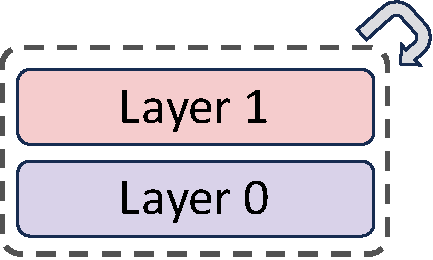
\includegraphics[width=0.91\linewidth]{figs/sharing_strategy/sharing_strategy_cycle.pdf}}
& \!\!\!$f\!\Bigl(\mathbf{h}_t^{\ell}; \Phi'_{(\ell - 1 \bmod ((L-2)/N_r)) + 1}\Bigr)$ 
& \multirow{-3}{*}{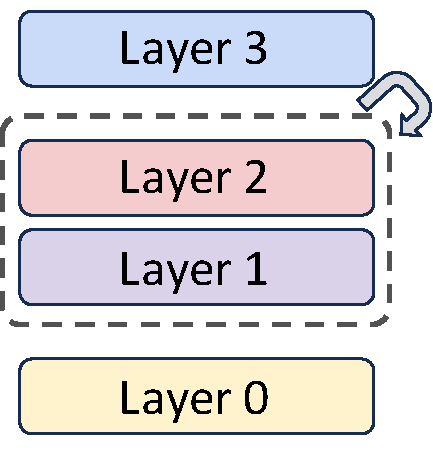
\includegraphics[width=0.91\linewidth]{figs/sharing_strategy/sharing_strategy_middle_cycle.pdf}} \\
[18pt]
First 
& -- 
& 
& $f\bigl(\mathbf{h}_t^{0}; \Phi_0\bigr)$ 
& \\ [5pt]
\midrule
% & \multicolumn{4}{c}{} \\[-15pt] % 약간 띄우기
% \midrule
& \multicolumn{2}{c|}{\textbf{Sequence Strategy}} & \multicolumn{2}{c}{\textbf{Middle-Sequence Strategy}} \\
\cmidrule(l{2pt}r{2pt}){2-3}\cmidrule(l{2pt}r{2pt}){4-5}
\textbf{Layers} & Equation & Figure & Equation & Figure \\
\midrule
Last 
& -- 
& 
& $f\bigl(\mathbf{h}_t^{L-1}; \Phi_{L-1}\bigr)$ 
& \\
[10pt]
Recursion 
& $f\!\Bigl(\mathbf{h}_t^{\ell}; \Phi'_{ \lfloor{\ell / N_r \rfloor}}\Bigr)$ 
& \multirow{-2}{*}{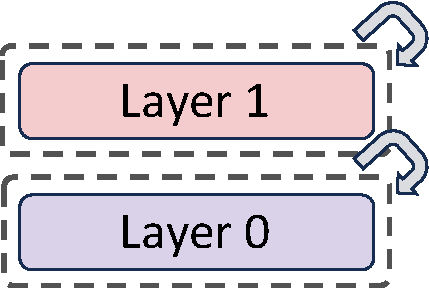
\includegraphics[width=0.91\linewidth]{figs/sharing_strategy/sharing_strategy_sequence.pdf}} 
& $f\!\Bigl(\mathbf{h}_t^{\ell}; \Phi'_{\lfloor(\ell - 1) / N_r\rfloor + 1)}\Bigr)$ 
& \multirow{-3}{*}{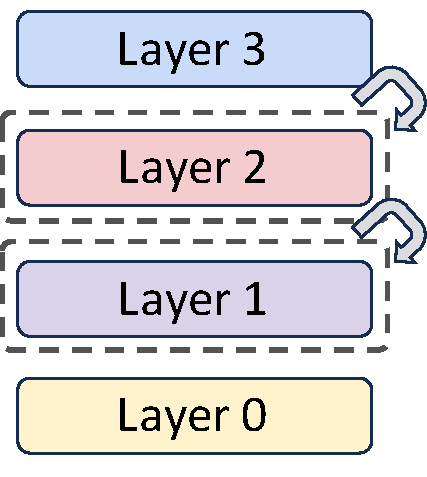
\includegraphics[width=0.91\linewidth]{figs/sharing_strategy/sharing_strategy_middle_sequence.pdf}} \\
[20pt]
First 
& -- 
& 
& $f\bigl(\mathbf{h}_t^{0}; \Phi_0\bigr)$ 
& \\[7pt]
\bottomrule
\end{tabular}
}
\end{table*}


\clearpage
\subsection{Routing Strategy}
In this section, we provide an in-depth explanation of the two routing strategies employed in Mixture-of-Recursions: \textit{Expert-choice} and \textit{Token-choice} routers. Each approach has distinct advantages and inherent limitations, which we first outline before discussing the mitigation techniques we utilized.


\vspace{-10pt}
\paragraph{Expert-choice routing.}
The expert-choice router offers several advantages, including a fixed compute budget that simplifies resource management. However, it suffers from a key issue: the top-$k$ selection operation, which requires information of tokens that appear later in the sequence, violates causality in autoregressive inference. This non-causal dependency (i.e., information leakage) can cause unexpected behavior during inference, potentially reducing model reliability. 

To address these challenges, we explore two approaches: the auxiliary router and the auxiliary loss \citep{raposo2024mixture}. The \textbf{auxiliary router} is an additional lightweight network trained jointly but used only during inference; it predicts whether a token will be among the top-$k$ selection. This additional router is trained with a binary cross-entropy loss, where the top-k selections from the main router are defined as the targets. Importantly, its training is isolated from the main objective through gradient blocking, so it does not affect the primary model training. Meanwhile, the \textbf{auxiliary loss} applies the binary cross-entropy loss to the main router itself, enabling it to simultaneously learn to push top-$k$ tokens towards one and others towards zero during training. This ensures the router can reliably predict which tokens will be selected as top-$k$ during inference.


\vspace{-10pt}
\paragraph{Token-choice routing.}
In contrast, the token-choice router assigns recursion depths on a per-token basis without enforcing a fixed compute budget, thus avoiding leakage of information across tokens and preserving autoregressive properties. However, this introduces load imbalance across experts, which results in uneven token distribution across experts (or recursion depths), potentially causing inefficient compute allocation and unbalanced training.

To mitigate load imbalance, we employ two solutions from existing literature. \textbf{Balancing Loss}~\citep{lepikhin2020gshard, fedus2022switch} regularizes for a more uniform distribution of tokens across experts. For a sequence of length $T$, a balancing loss for MoR is calculated as follows: 
\begin{equation*}
\begin{aligned}
\mathcal{L}_{\text{Balance}} &= \alpha \sum_{i=1}^{N_r} f_i P_i, \\
f_i &= \frac{N_r}{T} \sum_{t=1}^T \mathbb{I}(\text{Token } t \text{ selects Expert } i), \\
P_i &= \frac{1}{T} \sum_{t=1}^T g_t^i,
\end{aligned}
\end{equation*}
where $N_r$ is the total number of experts (which is also the number of recursion), $g_t^i$ is the routing score of expert $i$ for token $t$, $f_i$ represents the fraction of tokens routed to expert $i$, $P_i$ denotes the average routing scores of expert $i$, and $\lambda$ is a hyperparameter controlling the strength of the auxiliary loss.\looseness=-1

\textbf{Loss-free}~\citep{wang2024auxiliary} utilizes router biasing without explicit regularization loss. Specifically, this method adjusts per-expert bias terms \(b_i\) to balance token assignments across experts. During each training batch, routing scores are computed, and the number of tokens assigned to each expert ($c_i$) is counted. The load violation error is calculated as $e_i = \bar{c}_i - c_i$ where \(\bar{c}_i\) is the average token count for expert \(i\). Biases are then updated via $b_i \leftarrow b_i + u \times \operatorname{sign}(e_i)$, where \(u\) is a bias update rate.
The biased routing scores for selecting top-$k$ expert are calculated as
\begin{equation*}
g_{i}^t =
\begin{cases}
g_{i}^t, & \text{if } g_{i}^t + b_i \in \texttt{topk}\left(\{g_{j}^t + b_j \mid 1 \leq j \leq N\}, k\right) \\
0, & \text{otherwise}
\end{cases}
\end{equation*}
Note that the expert bias term is only utilized to adjust the routing strategy by influencing the top-$k$ selection.



\clearpage
\subsection{KV Caching Strategy}
This work investigates two principal strategies for key-value (KV) caching to optimize memory usage during Recursive Transformer computations: \textit{recursion-wise caching} and \textit{recursive KV sharing}.

\vspace{-10pt}
\paragraph{Recursion-wise caching.} This keeps separate KV caches for each recursion step, ensuring tokens attend only to the KV pairs generated in their current recursion block. This prevents distribution mismatches between recursion steps, helping to maintain model accuracy while reducing memory and computational costs.


\vspace{-10pt}
\paragraph{Recursive KV sharing.} In contrast, recursive sharing reuses KV pairs computed in the first recursion step for all subsequent steps. Although this approach further lowers memory usage and eliminates the need to compute deeper recursion during the prefill phase, it introduces potential mismatches as later recursion steps receive KV representations originally intended for earlier steps. Such mismatch can negatively impact model performance when token routing is precise.
Therefore, recursion-wise caching is generally preferred in settings with selective token routing to avoid performance degradation, while recursive KV sharing may be considered when memory efficiency is prioritized and prefill time is main bottleneck in the system.



\section{Experimental Setup}
\label{app:experimental_setup}


\paragraph{Training settings.}
We utilized a Llama-based Transformer architecture~\citep{grattafiori2024llama}, referring to the configurations of the open-source SmolLM models~\citep{allal2024SmolLM}. All models were pretrained on a deduplicated subset of the FineWeb-Edu dataset~\citep{penedo2024the} in SmolLM-Corpus~\citep{benallal2024smollmcorpus}, which comprises 220 billion tokens sourced from educational materials. Pretraining was conducted using four H100 or A100 GPUs. 
In our main and isoFLOPs analysis experiments, we utilized a Trapezoid learning rate scheduler, which consists of warmup (about 5\%), stable, and cooldown (20\%) phases. This approach allows us to efficiently continue pretraining for scaling laws from intermediate checkpoints, eliminating the need to train all models independently. In contrast, for all other experiments, we used a simple cosine annealing scheduler.


\vspace{-10pt}
\paragraph{Evaluation settings.}

To assess model performance, we evaluated few-shot accuracy on six benchmarks using the Language Model Evaluation Harness: LAMBADA (LD), HellaSwag (HS), PIQA (PQ), WinoGrande (WG), ARC (Easy and Challenge), and MMLU. For all few-shot datasets, excluding LAMBADA, WinoGrande, and MMLU, we normalized accuracy by the byte length of the target string. We adhered to the standard number of shots for each dataset, and used the continuation task specifically for MMLU for simplicity. 
All evaluation performance measurements were conducted using a single H100 or A100 GPU.


\vspace{-10pt}
\paragraph{Model architecture details.}

\autoref{tab:model_arch} summarizes the architectural specifications of the four Vanilla Transformer models used as the base for our recursive models. Each model variant differs in scale, ranging from 135M to 1.7B total parameters (including both non-embedding and embedding components). For consistency and comparability, all models are trained using a vocabulary size of 49K and a maximum input sequence length of 2K tokens.



\begin{table*}[h!]
    \caption{
    Key parameters of four model size variants. A model's size is defined by the total number of its non-embedding and embedding parameters. Three small models utilize Grouped-Query Attention~\citep{DBLP:conf/emnlp/AinslieLJZLS23}, reducing the number of key-value heads. We refer to the base configurations of the open-sourced SmolLM models~\citep{allal2024SmolLM}.
    }
    \label{tab:model_arch}
    \small
    \centering
    \resizebox{\textwidth}{!}{
    \setlength{\tabcolsep}{10pt}
    \begin{tabular}{l|cccc|cccc|cc}
    \toprule
      &  \multicolumn{4}{c|}{\textbf{Base Configuration}} & \multicolumn{4}{c|}{\textbf{Attention \& Feed-Forward}} & \multicolumn{2}{c}{\textbf{Input}} \\
    \cmidrule(l{2pt}r{2pt}){2-5} \cmidrule(l{2pt}r{2pt}){6-9} \cmidrule(l{2pt}r{2pt}){10-11}
     \textbf{Models} & N-emb & Emb & $N_L$ & $d_{model}$ & $N_{head}$ & $N_{KV}$ & $d_{head}$ & $d_{inter}$ & Vocab & $L_{ctx}$  \\
    \midrule
    Vanilla 135M & 106M & 28M & 30 & 576 & \,\,\,9 & 3 & 64 & 1536 & 49K & 2K \\[1pt]
    Vanilla 360M & 315M & 47M & 32 & 960 & 15 & 5 & 64 & 2560 & 49K & 2K \\[1pt]
    Vanilla 730M & 654M & 75M & 26 & \!\!\!1536 & 24 & 8 & 64 & 4096 & 49K & 2K \\[1pt]
    Vanilla \,\,\,1.7B & 1.61B & \!\!\!101M & 24 & \!\!\!2048 & 32 & \!\!\!32 & 64 & 8192 & 49K & 2K \\[1pt]
    \bottomrule
    \end{tabular}
    }
\end{table*}


\clearpage
\section{Expanded Results of Main Experiments}
\label{app:main_results}


\subsection{Performance Validation at 1.7B Scale}

We validate our models by scaling up the size to 1.7B, all under the same FLOPs budget. As shown in \autoref{tab:main_results_1_7b}, the MoR model with expert-choice routing shows strong performance, but the vanilla model performs slightly better. While this could be due to the differences in the optimal number of tokens associated with each model's optimal scaling policy, it might also signal that the current architecture design of MoR is not suitable for scaling. Nevertheless, we may be able to further improve performance by increasing the number of non-shared blocks (despite reduced efficiency), applying depth-specific LoRA or MoE to each recursion~\citep{bae2024relaxed}, or uptraining with initialization from a well-pretrained checkpoint. Further validation with larger sizes or training on more tokens is required. 




\begin{table*}[!h]
    \caption{
    Comparison of MoR, Recursive, and Vanilla Transformers at 1.7B scale under both fixed FLOPs (68.5e18) settings. All models are trained on FineWeb-Edu and evaluated by few-shot accuracy. For the isoFLOP rows, the number of training tokens\,($N_{tok}$) varies by model efficiency.
    For the model sizes, we report non-embedding parameter counts. $\text{}^\dagger$In recursive models, all tokens go through fixed recursion depths ($N_r$), instead of adaptive depths.
    \looseness=-1
    }
    \label{tab:main_results_1_7b}
    \small
    \centering
    \addtolength{\tabcolsep}{0pt}
    \resizebox{\textwidth}{!}{
    \begin{tabular}{l|cc|cc|ccc|cccccc|c}
    \toprule
      &  \multicolumn{2}{c|}{\textbf{MoR}} &  \multicolumn{2}{c|}{\textbf{Recursion}} & \multicolumn{3}{c|}{\textbf{Pretrain}} & \multicolumn{7}{c}{\textbf{Few-shot Accuracy\,$\uparrow$}} \\
    \cmidrule(l{2pt}r{2pt}){2-3} \cmidrule(l{2pt}r{2pt}){4-5} \cmidrule(l{2pt}r{2pt}){6-8} \cmidrule(l{2pt}r{2pt}){9-15} 
     \textbf{Models} & Type & KV & Share & $N_r$ & Param & FLOPs & $N_{tok}$  & LD & HS & PQ & WG & ARC & \!MMLU\! & Avg  \\
    \midrule
    Vanilla & - & - & - & -  & 1.61B &  68.5 & 20B & 40.8 & \textbf{49.4} & \textbf{70.6} & 54.8 & \textbf{47.4} & 30.2 & \textbf{48.9} \\
    \midrule
    \multirow{2}{*}{$\text{Recursive}^{\dagger}$} & - & -  & M-Cyc  & 2 & 0.87B & 68.5 & 18B  & 37.3 & 46.5 & 68.9 & 52.6 & 44.2 & 29.6 & 46.5 \\
     & - & - & M-Cyc & 3 & 0.67B & 68.5 & 20B & 36.4 & 45.3 & 69.5 & 52.7 &  43.9 & 29.1 & 46.2 \\
     \midrule
    & Expert & Cache  & M-Cyc  & 2 & 0.87B & 68.5 & 26B & \textbf{41.1} & 47.5 & 70.0 & \textbf{55.6} & 46.0 & \textbf{30.3} & 48.4 \\
     & Expert & Cache & M-Cyc & 3& 0.67B & 68.5 & 27B  & 37.2 & 46.6& 69.1 & 53.7 & 44.1 & 29.7 & 46.7 \\
     \cmidrule(l{2pt}r{2pt}){2-15}
     \multirow{-3.5}{*}{MoR\,(ours)} & Token & Cache & M-Cyc & 3& 0.67B & 68.5  & 30B & 35.6 & 43.2& 68.1 & 53.0 & 43.4 & 29.0 & 45.4 \\
    \bottomrule
    \end{tabular}
    }
\end{table*}


\subsection{Increasing Recursion Depth under Fixed Parameters}

\autoref{tab:recursion_number_under_same_param} illustrates the performance change when the number of recursions ($N_r$) is increased while the number of unique parameters is fixed at 118M. As the number of recursions rises from 1 (Vanilla) to 2 and 3 (MoR), the negative log-likelihood decreases on both the train and validation sets, and the average few-shot accuracy improves. This demonstrates that the MoR model can effectively scale performance by merely increasing the recursion steps, even with a fixed model size.


\begin{table*}[h!]
    \caption{
    Comparison of MoR with different numbers of recursions under the same number of parameters. Vanilla equals MoR with recursion 1. All models are trained on FineWeb-Edu with 10B tokens, and we apply the Middle-Cycle parameter sharing for MoR models. We report negative log-likelihood (NLL) on the train and validation sets and few-shot accuracy across six benchmarks. 
    }
    \label{tab:recursion_number_under_same_param}
    \small
    \centering
    \resizebox{\linewidth}{!}{
    \setlength{\tabcolsep}{4pt}
    \begin{tabular}{l|ccc|cc|cc|cccccc|c}
    \toprule
      & \multicolumn{3}{c|}{\textbf{Pretrain}} & \multicolumn{2}{c|}{\textbf{Recursion}} & \multicolumn{2}{c|}{\textbf{NLL\,$\downarrow$}} & \multicolumn{7}{c}{\textbf{Few-shot Accuracy\,$\uparrow$}} \\
    \cmidrule(l{2pt}r{2pt}){2-4} \cmidrule(l{2pt}r{2pt}){5-6} \cmidrule(l{2pt}r{2pt}){7-8} \cmidrule(l{2pt}r{2pt}){9-15}
    \textbf{Models} & N-Emb & $N_L$ & $N_{tok}$ & $N_r$ & Share & Train & Valid & LD & HS & PQ & WG & ARC & \!\!MMLU & Avg  \\ 
    \midrule
Vanilla & 118M & 12 & 10B &  1 & - & 2.9182 &  2.9678 & 25.81 & 33.08 & 61.81 & 51.46 & 38.10 & 26.64 & 39.48  \\
MoR & 118M  & 1+10+1 & 10B & 2 & M-Cyc &  2.8767 &  2.9205 & 27.09 & 33.84 & 62.13 & 53.04 & 36.77 & 26.88 & 39.96  \\
MoR & 118M  & 1+10+1 & 10B & 3 & M-Cyc & 2.8667 &  2.9111 & 27.38 & 34.60 & 63.17 & 51.46 & 37.15 & 26.83 & 40.10\\
    \bottomrule
    \end{tabular}
    }
\end{table*}


\clearpage
\section{Expanded Results of IsoFLOP Analysis}
\label{app:scaling_laws}


In the main paper (\S\ref{subsec:scaling_laws}), we compared Vanilla, Recursive and our Mixture‑of‑Recursions (MoR) models under matched \emph{training compute}. 
Four base model capacities were studied—135M, 360M, 730M and 1.7B parameters. 
For recursive and MoR models, we fix the recursion count to $N_r\!=\!3$, so the number of \emph{unique} parameters is roughly one‑third of the vanilla counterpart.  
Each architecture is trained once for the \emph{largest} compute budget (16.5EB)\footnote{1EB $\,{=}\,10^{18}$ floating‑point operations.} and the resulting checkpoint is re‑used to obtain the 5EB and 2EB variants, as detailed below.


\vspace{-10pt}
\paragraph{FLOPs approximated calculation of Transformers.}

We follow the approximation for calculating FLOPs as detailed in \citet{kaplan2020scaling}. Our analysis solely focuses on forward pass FLOPs, since the FLOPs involved in the backward pass are typically just double those of the forward pass. For most operations within Transformers, which primarily consist of linear projections, the forward pass FLOPs are calculated as two times the number of parameters, excluding the attention mechanism.

Regarding attention, we specifically account for the operations from the dot product between queries and keys and the scaling of values with softmax values. We only calculate FLOPs that contribute to the actual loss, excluding redundant computations in the upper triangular portion due to causality masking. Furthermore, we omit any additional computational costs associated with FlashAttention~\citep{dao2022flashattention}, normalization, and non-linearity operations from our overall FLOPs calculation.

As a result, Vanilla and Recursive Transformers have the same FLOPs. For MoR, the FLOPs calculation varies based on the routing and KV caching strategy. Especially, we calculated FLOPs based on the sequence length at each recursion depth, which is determined by the capacity factor and caching mechanism. In the case of token-choice routing, since the actual token allocation changes at every step, we approximated the FLOPs by assuming perfect balancing.
Furthermore, we add extra layers to a few MoR models to ensure their effective depth is divisible by the recursion number. For example, in a 135M model with 30 layers, setting a base depth of 10 and applying recursion three times (as in the Middle-Cycle strategy) results in a total of 32 layers. These additional layers introduce extra FLOPs, so we reduce the number of training steps accordingly to maintain our predefined FLOP budget.



\vspace{-10pt}
\paragraph{Trapezoid learning‑rate schedule with checkpoint reuse.}
To avoid retraining every model from scratch for each FLOPs budget, we employ the \textit{trapezoid} schedule~\citep{xing2018walk}. The rule of this scheduler is as follows:\looseness=-1
\begin{equation*}
\eta(t)=
\begin{cases}
\frac{t}{w}\,\eta_{\max}, & 0 \le t < w             \quad\text{(warm‑up)},\\[4pt]
\eta_{\max},                            & w \le t < p             \quad\text{(plateau)},\\[2pt]
\eta_{\max}\!\Bigl(1-\tfrac{t-p}{d}\Bigr), & p\le t < p+d \quad\text{(cool‑down)},
\end{cases}
\end{equation*}

where $w$ denotes the warm‑up interval, $p-w$ is the constant‑LR plateau, and $d$ represents the cool-down segment. This stable phase allows us to efficiently manage experiments by saving intermediate checkpoints and then running additional cool-down steps from those points, according to each budget. For the warmup, we allocate \(5\,\%\) of the total training steps of the smallest budget (2EB), and we set the cool‑down steps to \(20\,\%\) of the total training steps for each \emph{corresponding} budget.


\clearpage
\paragraph{Results at a glance.}
Table~\ref{tab:scaling_laws} reports NLL on FineWeb-Edu validation set and few‑shot accuracy on six benchmarks. Our findings reveal a clear trend: more compute consistently leads to better models, evidenced by lower NLL and improved accuracy with higher FLOPs. However, weight-sharing alone in recursive models degraded performance compared to Vanilla, a clear trade-off for the reduced parameters. Crucially, token-routed MoR models overcome this shortcoming, catching up to and then surpassing Vanilla models from 360M parameters upward, all while utilizing only one-third of the parameters. This performance advantage persists at 730M and 1.7B parameter scales.\looseness=-1


\begin{table*}[h!]
    \caption{Detailed results of isoFLOP analysis across three compute budgets. We evaluate negative log‑likelihood (NLL) on the FineWeb‑Edu validation set and few‑shot accuracy on six downstream tasks for four base model sizes (135M, 360M, 730M, 1.7B). Each model was initially trained up to 16.5EB and sliced back to 5EB and 2EB via mid‑training checkpoints using a trapezoid learning‑rate schedule. All models used three recursion steps. For MoR models, we use expert-choice routing and recursion-wise caching mechanisms. We highlight the best-performing model in each setting in gray.
    }

    \label{tab:scaling_laws}
    \small
    \centering
    \resizebox{\textwidth}{!}{
    \setlength{\tabcolsep}{4pt}
    \begin{tabular}{lc|cccc|cc|c|cccccc|c}
    \toprule
      & & \multicolumn{4}{c|}{\textbf{Pretrain}} &  \multicolumn{2}{c|}{\textbf{Recursion}} & \textbf{NLL\,$\downarrow$} & \multicolumn{7}{c}{\textbf{Few-shot Accuracy\,$\uparrow$}} \\
    \cmidrule(l{2pt}r{2pt}){3-6} \cmidrule(l{2pt}r{2pt}){7-8} \cmidrule(l{2pt}r{2pt}){9-9} \cmidrule(l{2pt}r{2pt}){10-16}
     \textbf{Models} & \textbf{Base} & N-Emb  & $N_L$ & FLOPs & $N_{tok}$ & Share & Loop & FineWeb & LD & HS & PQ & WG & ARC & \!MMLU\! & Avg  \\
    \midrule
    \rowcolor[gray]{0.9}
    Vanilla & 135M & 106M & 30 & \,\,\,2.0e+18  & 6.5B  & -  & - & 3.0922 & 22.80 & 30.93 & 62.35 & 51.14 & 36.28 & 26.29 & 38.30  \\
    Recursive & 135M & \,\,\,42M & 1+10+1 & \,\,\,2.0e+18  & 6.1B & M-Cyc  & 3 & 3.2058 & 19.79 & 29.32 & 60.17 & 50.59 & 34.83 & 25.40 & 36.68  \\
    MoR & 135M & \,\,\,42M & 1+10+1 & \,\,\,2.0e+18  & 9.2B & M-Cyc  & 3 & 3.1077 & 21.13 & 31.00 & 59.79 & 49.09 & 34.87 & 25.63 & 36.92  \\
    \midrule
    \rowcolor[gray]{0.9}
    Vanilla & 135M & 106M & 30 &  \,\,\,5.0e+18   & \!\!\!16.1B & -  & - & 2.9464 & 26.88 & 33.69 & 63.98 & 51.46 & 37.08 & 27.07 & 40.03  \\
    Recursive & 135M & \,\,\,42M & 1+10+1  &  \,\,\,5.0e+18   & \!\!\!15.1B & M-Cyc  & 3 & 3.0534 & 24.51 & 31.57 & 62.40 & 50.83 & 35.78 & 25.94 & 38.51  \\
    MoR & 135M & \,\,\,42M & 1+10+1  &  \,\,\,5.0e+18   & \!\!\!23.1B & M-Cyc  & 3 & 3.0192 & 22.01 & 32.53 & 61.75 & 49.88 & 35.39 & 26.19 & 37.96  \\
    \midrule
    \rowcolor[gray]{0.9}
    Vanilla & 135M & 106M & 30 & 16.5e+18  & \!\!\!53.3B & -  & - & 2.8432 & 30.16 & 36.51 & 64.80 & 53.43 & 40.17 & 27.82 & 42.15  \\
    Recursive & 135M & \,\,\,42M & 1+10+1 & 16.5e+18  & \!\!\!50.0B & M-Cyc  & 3 & 2.9552 & 25.98 & 33.36 & 63.98 & 51.78 & 36.96 & 26.68 & 39.79  \\
    MoR & 135M & \,\,\,42M & 1+10+1 & 16.5e+18  & \!\!\!76.2B & M-Cyc  & 3 & 2.9490 & 22.61 & 33.99 & 61.92 & 47.83 & 35.95 & 26.36 & 38.11  \\
    \midrule
    \midrule
    Vanilla & 360M & 315M & 32 & \,\,\,2.0e+18   & 2.4B & -  & - & 3.3785 & 17.27 & 27.90 & 59.36 & 51.38 & 32.10 & 25.49 & 35.58  \\
    Recursive & 360M & 118M & 1+10+1 & \,\,\,2.0e+18   & 2.4B & M-Cyc  & 3 & 3.4864 & 10.34 & 26.66 & 58.00 & 51.54 & 30.94 & 24.94 & 33.74  \\
    \rowcolor[gray]{0.9}
    MoR & 360M & 118M & 1+10+1 & \,\,\,2.0e+18   & 3.6B & M-Cyc  & 3 & 3.1026 & 24.14 & 30.53 & 61.86 & 50.99 & 34.74 & 25.50 & 37.96  \\
    \midrule
    Vanilla & 360M & 315M & 32 &  \,\,\,5.0e+18   & 6.0B & -  & - & 3.0097 & 25.17 & 32.10 & 63.22 & 48.62 & 36.01 & 26.69 & 38.63  \\
    Recursive & 360M & 118M & 1+10+1 &  \,\,\,5.0e+18   & 6.0B & M-Cyc  & 3 & 3.0722 & 23.29 & 31.19 & 62.62 & 51.30 & 35.85 & 25.99 & 38.37  \\
    \rowcolor[gray]{0.9}
    MoR & 360M & 118M & 1+10+1 &  \,\,\,5.0e+18   & 9.0B & M-Cyc  & 3 & 2.9161 & 28.33 & 34.53 & 63.22 & 51.07 & 36.70 & 26.98 & 40.14  \\
    \midrule
    Vanilla & 360M & 315M & 32 & 16.5e+18  & \!\!\!19.8B & -  & - & 2.7824 & 31.94 & 37.92 & 66.10 & 51.30 & 39.70 & 27.95 & 42.49  \\
    Recursive & 360M & 118M & 1+10+1 & 16.5e+18  & \!\!\!19.8B & M-Cyc  & 3 & 2.8466 & 29.75 & 35.92 & 64.91 & 51.46 & 39.12 & 27.18 & 41.39  \\
    \rowcolor[gray]{0.9}
    MoR & 360M & 118M & 1+10+1 & 16.5e+18  & \!\!\!29.7B & M-Cyc  & 3 & 2.7924 & 33.15 & 37.94 & 66.97 & 52.09 & 38.46 & 27.49 & 42.68  \\
    \midrule
    \midrule
    Vanilla & 730M & 654M & 26 & \,\,\,2.0e+18   & 1.2B & -  & - & 3.7164 & 07.74 & 26.58 & 57.62 & 51.14 & 29.74 & 24.46 & 32.88  \\
    Recursive & 730M & 252M & 1+8+1 & \,\,\,2.0e+18   & 1.2B & M-Cyc  & 3 & 3.8136 & 05.53 & 26.25 & 55.77 & 50.59 & 29.88 & 24.63 & 32.11  \\
    \rowcolor[gray]{0.9}
    MoR & 730M & 252M & 1+8+1 & \,\,\,2.0e+18   & 1.8B & M-Cyc  & 3 & 3.3300 & 17.93 & 28.74 & 59.30 & 51.46 & 33.14 & 25.37 & 35.99  \\
    \midrule
    Vanilla & 730M & 654M & 26 &  \,\,\,5.0e+18   & 3.1B & -  & - & 3.0821 & 22.05 & 31.99 & 62.68 & 50.67 & 35.88 & 26.12 & 38.23  \\
    Recursive & 730M & 252M & 1+8+1 &  \,\,\,5.0e+18   & 3.1B & M-Cyc  & 3 & 3.1640 & 18.51 & 30.72 & 62.13 & 47.83 & 35.97 & 25.84 & 36.83  \\
    \rowcolor[gray]{0.9}
    MoR & 730M & 252M & 1+8+1 &  \,\,\,5.0e+18   & 4.5B & M-Cyc  & 3 & 3.0067 & 26.18 & 32.76 & 62.46 & 50.91 & 36.93 & 26.37 & 39.27  \\
    \midrule
    Vanilla & 730M & 654M & 26 & 16.5e+18  & \!\!\!10.1B & -  & - & 2.7048 & 34.50 & 40.29 & 66.81 & 49.49 & 40.82 & 28.66 & 43.43  \\
    Recursive & 730M & 252M & 1+8+1 & 16.5e+18  & \!\!\!10.1B & M-Cyc  & 3 & 2.7886 & 30.76 & 37.84 & 65.51 & 52.41 & 39.26 & 27.51 & 42.21  \\
    \rowcolor[gray]{0.9}
    MoR & 730M & 252M & 1+8+1 & 16.5e+18  & \!\!\!14.9B & M-Cyc  & 3 & 2.7438 & 32.93 & 39.55 & 66.32 & 54.38 & 40.00 & 28.09 & 43.55  \\
    \midrule
    \midrule
    Vanilla & \,\,\,1.7B & 1.61B & 24 & \,\,\,2.0e+18   & 0.6B & -  & - & 5.1349 & 00.00 & 24.96 & 51.03 & 51.38 & 25.75 & 23.07 & 29.37  \\
    Recursive & \,\,\,1.7B & 0.67B & 1+8+1 & \,\,\,2.0e+18   & 0.5B & M-Cyc  & 3 & 5.3277 & 00.00 & 25.27 & 51.36 & 48.62 & 26.52 & 22.98 & 29.13  \\
    \rowcolor[gray]{0.9}
    MoR & \,\,\,1.7B & 0.67B & 1+8+1 & \,\,\,2.0e+18   & 0.8B & M-Cyc  & 3 & 4.1175 & 01.44 & 25.80 & 53.97 & 49.64 & 27.56 & 24.08 & 30.42  \\
    \midrule
    Vanilla & \,\,\,1.7B & 1.61B & 24 &  \,\,\,5.0e+18   & 1.5B & -  & - & 3.6926 & 08.33 & 26.84 & 57.29 & 51.30 & 29.72 & 24.51 & 33.00  \\
    Recursive & \,\,\,1.7B & 0.67B & 1+8+1 &  \,\,\,5.0e+18   & 1.3B & M-Cyc  & 3 & 3.8876 & 03.14 & 26.57 & 54.73 & 49.17 & 29.01 & 24.49 & 31.19  \\
    \rowcolor[gray]{0.9}
    MoR & \,\,\,1.7B & 0.67B & 1+8+1 &  \,\,\,5.0e+18   & 2.0B & M-Cyc  & 3 & 3.2905 & 17.62 & 28.32 & 59.03 & 49.80 & 32.14 & 25.28 & 35.37  \\
    \midrule
    Vanilla & \,\,\,1.7B & 1.61B & 24 & 16.5e+18  & 4.8B & -  & - & 2.8658 & 26.94 & 35.61 & 64.74 & 50.59 & 38.55 & 26.81 & 40.54  \\
    Recursive & \,\,\,1.7B & 0.67B & 1+8+1 & 16.5e+18  & 4.5B & M-Cyc  & 3 & 3.0042 & 23.25 & 32.09 & 62.95 & 50.75 & 37.64 & 26.53 & 38.87  \\
    \rowcolor[gray]{0.9}
    MoR & \,\,\,1.7B & 0.67B & 1+8+1 & 16.5e+18  & 6.5B & M-Cyc  & 3 & 2.8316 & 28.10 & 36.18 & 64.64 & 50.99 & 38.68 & 27.25 & 40.97  \\
    \bottomrule
    \end{tabular}
    }
\end{table*}


\clearpage
\section{Details of Experimental Settings for Throughput Measurement}
\label{app:throughput}

We implement a continuous depth-wise batching inference system~\citep{bae2024relaxed, hooper2023speed} to evaluate decoding throughput of MoR models. Queries are enqueued and scheduled dynamically during decoding using 1K samples from the FineWeb-Edu validation set. In particular, for MoR, when some queries exit early, the vacant slots in the batch are immediately filled with new queries waiting in the queue, maintaining a fully utilized batch at all times.\looseness=-1


We compare the throughput of Vanilla and MoR models (at a 360M parameter scale) for generating a certain length of tokens per sample, where the number is sampled from a normal distribution with a mean of 256, starting without any input prefix. The speeds of the MoR models are normalized against the speed of the Vanilla Transformer. For pretraining MoR-4 models, we add two additional layers (34 layers in total) before applying recursion. This ensures the total effective depth is divisible by the recursion number (specifically for the Middle-Cycle strategy). Consequently, the speed comparison for MoR-4 is made against a modified vanilla model that includes these two extra layers, resulting in a total of 34 layers (32 original layers + 2 added layers).\looseness=-1


We use two batching settings: (1) a \textit{fixed batch size of 32} and (2) a \textit{relative maximum batch size}, derived by multiplying 32 by the ratio of the maximum batch sizes of vanilla and MoR models. Specifically, based on the H100 GPU's VRAM size, we calculated the maximum batch sizes by considering model parameters and their KV cache memory. For simplicity, we omit the memory size from the hidden states at the current position. Under these adaptive conditions, MoR-2 supports a batch size of 42, MoR-3 supports 48, and MoR-4 supports up to 51. By employing recursion-wise KV caching, MoR allows a substantial increase in batch size stemming from its reduced parameter and KV cache memory footprint. 


For implementation, we use a queue to enable continuous depth-wise batching and employ FlashAttention 2~\citep{dao2023flashattention} to support variable-length KV caches within a batch. We adopt a \textit{static}-sized cache where each position is updated over time, since this is compatible with \texttt{torch.compile}~\citep{paszke2019pytorch} to further optimize inference speeds. Furthermore, mimicking real-world deployment scenarios~\citep{kwon2023efficient, zhong2024distserve}, we decouple the transformer block phase from the rest of the computation by pre-processing the input embeddings or the first non-shared layer before passing into the transformer blocks. Then, we measured the actual time taken during the forward pass. Note that we include a warmup stage by running the model for 100 iterations before actual measurement, in order to obtain stable timing results. For further optimization, tokens that exited early were accumulated up to the maximum batch size before being processed by the last non-shared layer, classifier, and embedding layers (including the non-shared first layer in the case of MoR models). After this, we queue them for sequential batching by following a FIFO (First-In, First-Out) strategy. For implementation convenience, we exclude the time spent on caching and updating for KV pairs, as these aspects can be significantly optimized through various engineering techniques~\citep{kwon2023efficient}. We leave a more precise speed comparison, which accounts for these considerations, as future work.


\clearpage
\section{Expanded Results of Parameter Sharing Strategy}
\label{app:parameter_sharing}

This section complements the ablation in \S\ref{subsec:sharing} by providing the full quantitative panorama behind \autoref{fig:pareto_frontier_sharing-b}. We revisit the four weight‑tying schemes—\textit{Cycle}, \textit{Sequence}, \textit{Middle‑Cycle}, and \textit{Middle‑Sequence}—on two base model scales (135M and 360M non‑embedding parameters) and two different recursion depths ($N_{r}=2$ and~3). All models were trained from scratch for 10B tokens under identical optimization hyperparameters. Validation NLL on FineWeb‑Edu and averaged few‑shot accuracy over six benchmarks are summarized in \autoref{tab:revist_sharing_strategy}.


\vspace{-10pt}
\paragraph{Middle‑Cycle is consistently the safest choice.}
For the 360M models, Middle-Cycle achieves the lowest NLL at both depths ($N_{r}=2$ and $N_{r}=3$) and also shows the largest improvement in average accuracy compared to vanilla reduced models. For the 135M models, while Cycle is slightly ahead at two recursion setting (3.0071 vs. 3.0330), Middle-Cycle overtakes when recursion depth rises (3.1048 vs. 3.1154) and shows a steadier accuracy profile. Meanwhile, pure Sequence sharing records the worst NLL in all four settings, and its accuracy gap widens with recursion depth. The Middle strategy slightly improves the performance of the Sequence, but it still performs worse than the Cycle-based methodology. We visualized the results in \autoref{fig:revisit_sharing_app}.\looseness=-1


\begin{table*}[h!]
  \caption{
    Comparison of parameter-sharing strategies (Cycle, Sequence, Middle-Cycle, Middle-Sequence) across two model scales (135M and 360M) and two recursion depths ($N_R = 2$ and $N_R = 3$). All models are pretrained from scratch on 10B tokens. We report validation negative log-likelihood (NLL) on FineWeb-Edu and few-shot accuracy across six tasks. Middle-Cycle consistently outperforms other strategies in both NLL and average task accuracy, especially at higher recursion depth. We highlight the optimal strategy for each setting in gray.\looseness=-1
    }
  \label{tab:revist_sharing_strategy}
  \small
  \centering
  \resizebox{\textwidth}{!}{
  \setlength{\tabcolsep}{4pt}
  \begin{tabular}{l|ccc|cc|c|cccccc|c}
  \toprule
   & \multicolumn{3}{c|}{\textbf{Pretrain}} & \multicolumn{2}{c|}{\textbf{Recursion}} & \textbf{NLL\,$\downarrow$} & \multicolumn{7}{c}{\textbf{Few-shot Accuracy\,$\uparrow$}} \\
  \cmidrule(l{2pt}r{2pt}){2-4} \cmidrule(l{2pt}r{2pt}){5-6} \cmidrule(l{2pt}r{2pt}){7-7} \cmidrule(l{2pt}r{2pt}){8-14} 
    \textbf{Base Model} & N-Emb & $N_L$ & $N_{tok}$ & Share & Loop & FineWeb & LD & HS & PQ & WG & ARC & \!MMLU\! & Avg \\
  \midrule
  Vanilla\,135M & 106M & 30 & 10B & - & - & 3.0323 & 24.14 & 31.12 & 61.15 & 52.01 & 34.74 & 25.95 & 38.19 \\
  Vanilla\,135M & \,\,\,53M & 15 & 10B & - & - & 3.0818 & 23.64 & 30.10 & 60.94 & 50.99 & 35.38 & 25.93 & 37.83 \\
  Vanilla\,135M & \,\,\,35M & 10 & 10B & - & - & 3.1582 & 21.46 & 29.30 & 60.01 & 52.01 & 34.40 & 25.53 & 37.12 \\
  \midrule
  \rowcolor[gray]{0.9}
  Vanilla\,135M & \,\,\,53M & 15 & 10B & Cyc & 2 & 3.0071 & 25.52 & 31.25 & 61.10 & 50.99 & 36.08 & 26.11 & 38.51 \\
  Vanilla\,135M & \,\,\,53M & 15 & 10B & Seq & 2 & 3.1093 & 22.39 & 29.60 & 61.10 & 50.12 & 34.46 & 25.72 & 37.23 \\
   Vanilla\,135M & \,\,\,57M & 1+14+1 & 10B & M-Cyc & 2 & 3.0330 & 23.40 & 31.20 & 61.59 & 50.59 & 35.44 & 25.54 & 37.96 \\
    Vanilla\,135M & \,\,\,57M & 1+14+1 & 10B & M-Seq & 2 & 3.0991 & 21.70 & 30.06 & 60.45 & 49.41 & 35.20 & 25.74 & 37.09 \\
    \midrule
    Vanilla\,135M & \,\,\,35M & 10 & 10B & Cyc & 3 & 3.1154 & 21.42 & 30.14 & 60.61 & 49.72 & 34.15 & 25.57 & 36.94 \\
    Vanilla\,135M & \,\,\,35M & 10 & 10B & Seq & 3 & 3.1637 & 19.99 & 29.39 & 59.25 & 51.62 & 33.79 & 25.32 & 36.56 \\
    \rowcolor[gray]{0.9}
    Vanilla\,135M & \,\,\,39M & 1+9+1 & 10B & M-Cyc & 3 & 3.1048 & 22.41 & 30.35 & 61.04 & 49.01 & 34.80 & 25.91 & 37.26 \\
    Vanilla\,135M & \,\,\,39M & 1+9+1 & 10B & M-Seq & 3 & 3.1602 & 20.69 & 29.35 & 61.43 & 51.30 & 34.40 & 25.51 & 37.11 \\
    \midrule
    \midrule
    Vanilla\,360M & 315M & 32 & 10B & - & - & 2.8471 & 27.27 & 34.78 & 64.20 & 52.80 & 38.29 & 26.72 & 40.68 \\
    Vanilla\,360M & 157M & 16 & 10B & - & - & 2.8908 & 27.01 & 33.49 & 64.42 & 52.09 & 37.40 & 26.54 & 40.16 \\
    Vanilla\,360M & \,\,\,98M & 10 & 10B & - & - & 2.9449 & 26.41 & 32.93 & 63.38 & 50.36 & 37.15 & 26.48 & 39.45 \\
    \midrule
    Vanilla\,360M & 157M & 16 & 10B & Cyc & 2 & 2.8487 & 28.47 & 34.79 & 63.06 & 49.96 & 37.38 & 26.81 & 40.08 \\
    Vanilla\,360M & 157M & 16 & 10B & Seq & 2 & 2.9467 & 26.33 & 32.49 & 62.89 & 52.41 & 36.37 & 26.24 & 39.46 \\
    \rowcolor[gray]{0.9}
    Vanilla\,360M & 167M & 1+15+1 & 10B & M-Cyc & 2 & 2.8295 & 28.59 & 34.98 & 64.53 & 50.51 & 39.68 & 27.20 & 40.91 \\
    Vanilla\,360M & 167M & 1+15+1 & 10B & M-Seq & 2 & 2.9303 & 26.14 & 32.71 & 62.79 & 51.38 & 36.31 & 25.73 & 39.18 \\
    \midrule
    Vanilla\,360M & \,\,\,98M & 10 & 10B & Cyc & 3 & 2.9363 & 25.87 & 32.98 & 62.89 & 50.28 & 36.35 & 26.54 & 39.15 \\
    Vanilla\,360M & \,\,\,98M & 10 & 10B & Seq & 3 & 3.0245 & 24.55 & 31.48 & 63.11 & 49.25 & 35.65 & 25.73 & 38.30 \\
    \rowcolor[gray]{0.9}
    Vanilla\,360M & 118M & 1+10+1 & 10B & M-Cyc & 3 & 2.8760 & 28.51 & 34.89 & 64.31 & 50.51 & 39.51 & 27.20 & 40.82 \\
    Vanilla\,360M & 118M & 1+10+1 & 10B & M-Seq & 3 & 2.9753 & 24.18 & 31.89 & 62.08 & 49.72 & 36.47 & 26.27 & 38.44 \\
    \bottomrule
  \end{tabular}
  }
  
\end{table*}


\clearpage

\begin{figure}[h]
    \centering
    \begin{subfigure}[t]{0.35\textwidth}
    \captionsetup{justification=centering}
        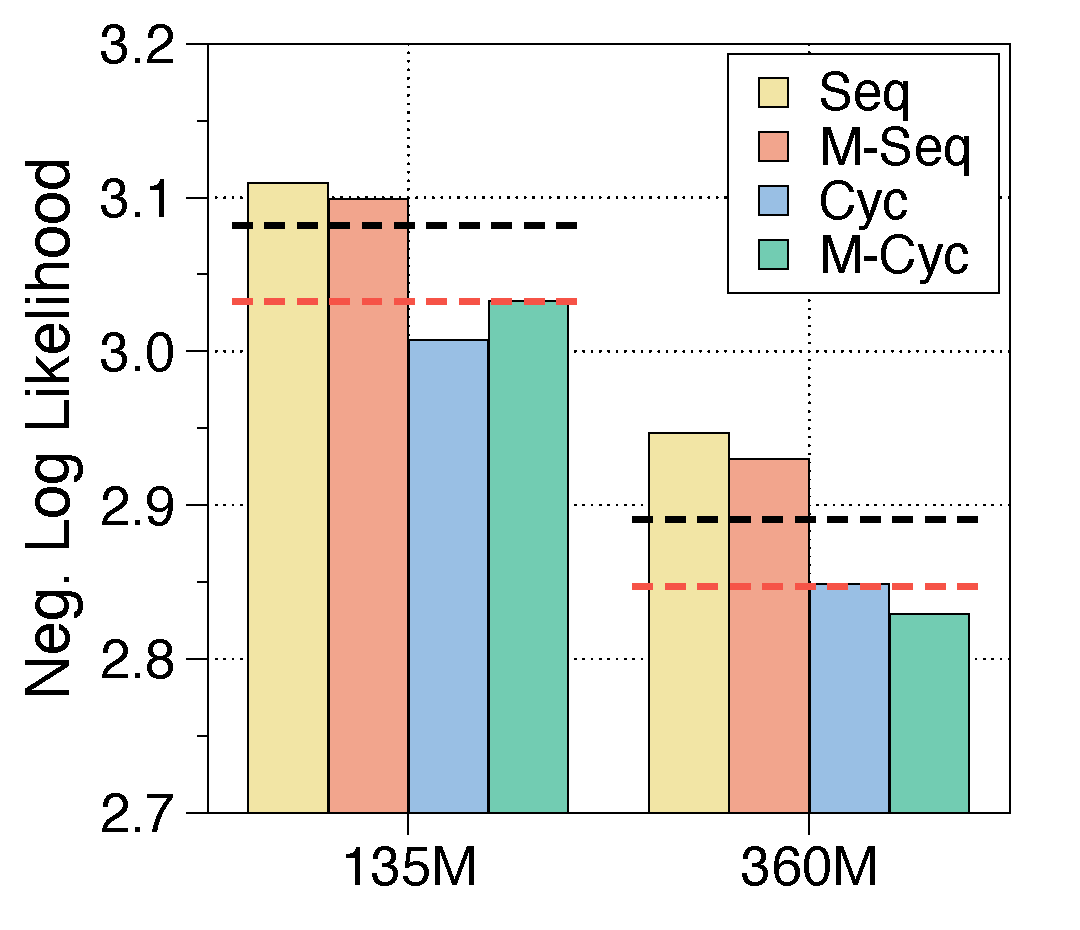
\includegraphics[width=\textwidth]{figs/revisit_sharing/revisit_sharing_rec2.pdf}
        \subcaption{Recursion of two\,($N_R$ = 2)}
        \label{fig:revisit_sharing_rec2_app}
    \end{subfigure}
    \hspace{10pt}
    \centering
    \begin{subfigure}[t]{0.35\textwidth}
    \captionsetup{justification=centering}
        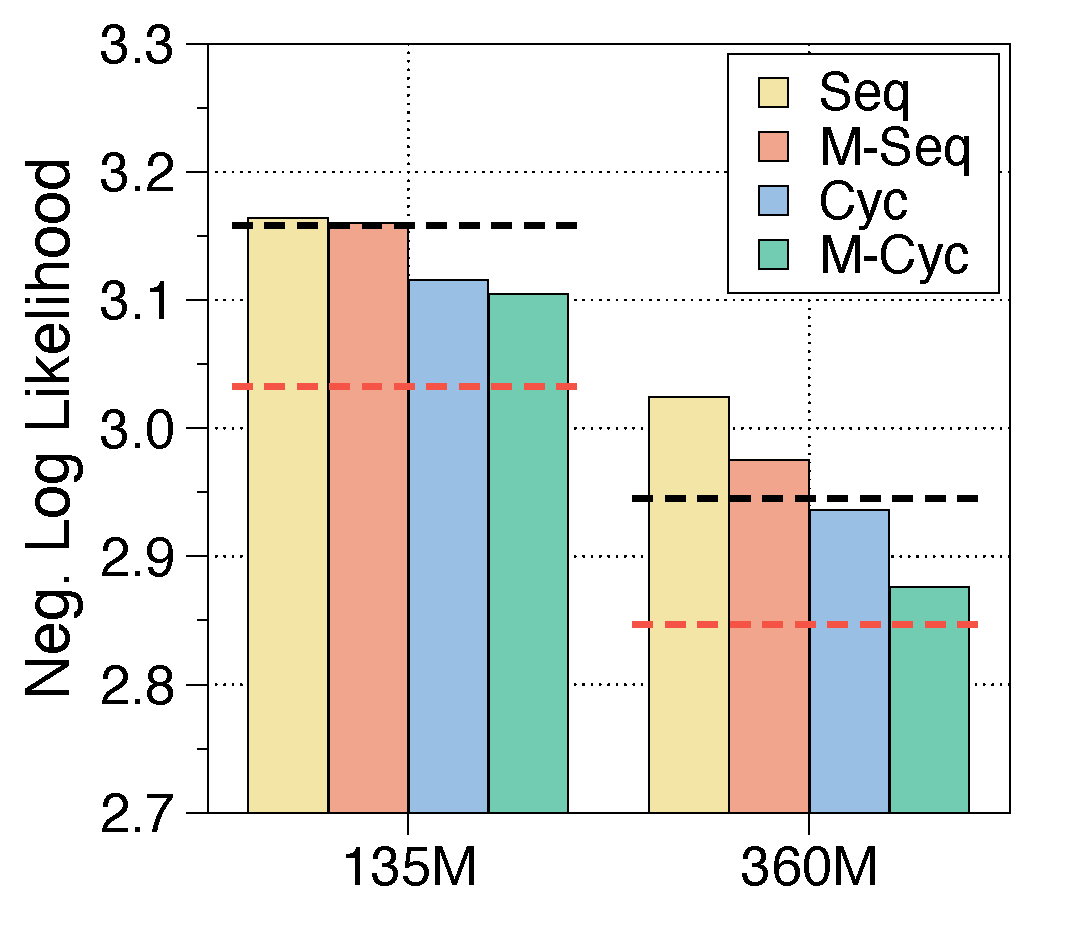
\includegraphics[width=\textwidth]{figs/revisit_sharing/revisit_sharing_rec3.pdf}
        \subcaption{Recursion of three\,($N_R$ = 3)}
        \label{fig:revisit_sharing_rec3_app}
    \end{subfigure}
    \caption{
    Validation negative log‑likelihood (lower is better) on \emph{FineWeb‑Edu} for four parameter‑sharing strategies.
    Bars are grouped by model capacity (135M vs.\ 360M parameters). 
    Middle‑Cycle consistently attains the lowest NLL, with its margin widening as either model size or depth increases.
    The horizontal dashed lines mark the \emph{untied} (non-sharing) baselines: the lower red line represents the full capacity model, while the upper black line represents a parameter-matched reduced model with a footprint equal to the unique trainable parameter sizes of the recursive model.
    }
    \label{fig:revisit_sharing_app}
\end{figure}



For fairer comparison, we also compare the Middle-Cycle and Cycle sharing strategies, fixing the number of unique parameters for both models. For 730M model comparison, both strategies use 3 recursion steps. Especially, Middle-Cycle uses 8 layers for the recursion block and 2 unshared layers (1 + 8$\times$3 + 1), resulting in 10 unique layers and 26 effective layers. We compare this to the Cycle strategy with 10 layers per recursion block (10$\times$3), which also has 10 unique layers but a total of 30 effective layers. Despite having fewer effective layers, as shown in \autoref{tab:m_cycle_cycle_compare}, the Middle-Cycle model achieves better performance, with a lower negative log-likelihood (2.7552 vs. 2.7573) and higher average few-shot accuracy (42.32 vs. 41.90). While these results are promising, we leave further validation across more scales as future work. 

\begin{table*}[h!]
    \caption{
    Comparison of Middle-Cycle and Cycle sharing strategies under the same number of unique parameters. All models use 730M scales (non-embedding parameters) as the base model with 3 recursion steps. The models are trained from scratch on 10B tokens using the Fineweb-Edu dataset.
    }
    \label{tab:m_cycle_cycle_compare}
    \small
    \centering
    \resizebox{\linewidth}{!}{
    \setlength{\tabcolsep}{4pt}
    \begin{tabular}{l|cc|ccc|c|cccccc|c}
    \toprule
      & \multicolumn{2}{c|}{\textbf{Recursion}} & \multicolumn{3}{c|}{\textbf{Pretrain}} & \textbf{NLL\,$\downarrow$} & \multicolumn{7}{c}{\textbf{Few-shot Accuracy\,$\uparrow$}} \\
    \cmidrule(l{2pt}r{2pt}){2-3} \cmidrule(l{2pt}r{2pt}){4-6} \cmidrule(l{2pt}r{2pt}){7-7} \cmidrule(l{2pt}r{2pt}){8-14}
    \textbf{Base Model} & Share & Loop & N-Emb\!\! & $N_L$ & $N_{tok}$ & Fineweb & LD & HS & PQ & WG & ARC & \!\!MMLU & Avg  \\ 
    \midrule
Vanilla 730M & Cycle & 3 & 252M & 10 & 10B & 2.7573 &  28.72 & 37.31 & 65.56 & 52.01 & 39.94 & 27.85 & 41.90 \\
Vanilla 730M & M-Cycle & 3 & 252M & 1+8+1 & 10B & 2.7552 & 29.75 & 37.73 & 66.00 & 52.49 & 40.49 & 27.50 & 42.32 \\
    \bottomrule
    \end{tabular}
    }
\end{table*}


\clearpage
\paragraph{Behavior under continued pre‑training (up‑training).}
\autoref{tab:revist_sharing_strategy_uptrain} extends the study by ``up‑training'' models---continuing from open-sourced SmolLM~\citep{allal2024SmolLM} checkpoints for an additional 5B tokens.
Both Middle strategies demonstrate superior performance across all settings, and notably, they significantly outperform the reduced baseline models that are initialized in the same manner but without recursion.
The other strategies reach a performance plateau earlier, suggesting that they have limited room for further improvement in capacity.








\begin{table*}[h!]
    \caption{
    Uptraining results across four parameter sharing strategies. Models are trained on 5B tokens from FineWeb-Edu and evaluated by train NLL and few-shot accuracy across six benchmarks. ARC denotes average of ARC-Easy and ARC-Challenge tasks, MMLU denotes the MMLU-Cont task. We highlight the optimal strategy for each setting in gray.\looseness=-1
    }
    \label{tab:revist_sharing_strategy_uptrain}
    \small
    \centering
    \resizebox{\textwidth}{!}{
    \setlength{\tabcolsep}{3pt}
    \begin{tabular}{l|ccc|ccc|c|cccccc|c}
    \toprule
      &  \multicolumn{3}{c|}{\textbf{Pretrain}} &  \multicolumn{3}{c|}{\textbf{Recursion}} & \textbf{NLL\,$\downarrow$} & \multicolumn{7}{c}{\textbf{Few-shot Accuracy\,$\uparrow$}} \\
    \cmidrule(l{2pt}r{2pt}){2-4} \cmidrule(l{2pt}r{2pt}){5-7} \cmidrule(l{2pt}r{2pt}){8-8} \cmidrule(l{2pt}r{2pt}){9-15} 
     \textbf{Base Model} & N-Emb & $N_L$ & $N_{tok}$ & Share & Init & Loop & FineWeb & LD & HS & PQ & WG & ARC & \!MMLU\! & Avg  \\
    \midrule
    Vanilla\,360M & 315M & 32 & 5B & -  & - & -  & 2.4825 & 41.67 & 50.63 & 70.35 & 55.09 & 46.99 & 30.82 & 49.26  \\
    Vanilla\,360M & 157M & 16 & 5B & - & Step  & 1   & 2.7168 & 31.85 & 37.59 & 64.74 & 53.20 & 41.06 & 27.34 & 42.63  \\
    Vanilla\,360M & 157M & 16 & 5B & Cyc  & Avg & 1  & 2.8603 & 22.14 & 30.36 & 60.07 & 48.22 & 34.99 & 25.56 & 36.89  \\
    Vanilla\,360M & 157M & 16 & 5B & Seq  & Avg & 1  & 2.7919 & 25.40 & 32.35 & 62.30 & 50.12 & 35.88 & 26.19 & 38.71  \\
    Vanilla\,360M & \,\,\,98M & 10 & 5B & -  & Step & 1  & 2.8915 & 26.63 & 35.03 & 64.42 & 52.09 & 38.75 & 26.86 & 40.63    \\
    Vanilla\,360M & \,\,\,98M & 10 & 5B & Cyc  & Avg & 1  & 3.0512 & 23.19 & 31.27 & 62.30 & 51.22 & 36.71 & 26.29 & 38.50   \\
    Vanilla\,360M & \,\,\,98M & 10 & 5B & Seq  & Avg & 1  & 2.9915 & 25.67 & 32.21 & 62.30 & 51.38 & 36.68 & 26.56 & 39.14  \\
    \midrule
     \rowcolor[gray]{0.9}
    Vanilla\,360M & 157M & 16 & 5B & Cyc  & Step & 2  & 2.7165 & 31.30 & 37.68 & 64.91 & 52.17 & 39.29 & 27.53 & 42.15  \\
    Vanilla\,360M & 157M & 16 & 5B & Cyc  & Avg & 2  & 2.8263 & 23.21 & 30.52 & 60.55 & 50.28 & 36.01 & 25.50 & 37.68  \\
    Vanilla\,360M & 157M & 16 & 5B & Cyc  & Lower & 2  & 2.8024 & 27.67 & 34.71 & 63.49 & 49.88 & 38.12 & 26.87 & 40.13  \\
    Vanilla\,360M & 157M & 16 & 5B & Cyc  & Upper & 2  & 2.7915 & 18.26 & 34.88 & 63.06 & 51.85 & 39.27 & 26.88 & 39.03  \\
    Vanilla\,360M & 157M & 16 & 5B & Cyc  & Rand & 2  & 2.7575 & 25.29 & 34.78 & 61.64 & 52.01 & 38.09 & 26.62 & 39.74   \\
    \midrule
     \rowcolor[gray]{0.9}
    Vanilla\,360M & 157M & 16 & 5B & Seq  & Step & 2  & 2.6862 & 34.14 & 42.49 & 67.90 & 53.35 & 43.24 & 28.80 & 44.99  \\
    Vanilla\,360M & 157M & 16 & 5B & Seq  & Avg & 2  & 2.7508 & 29.01 & 34.13 & 63.60 & 52.09 & 36.31 & 26.58 & 40.29  \\
    Vanilla\,360M & 157M & 16 & 5B & Seq  & Lower & 2  & 2.8300 & 27.50 & 33.28 & 63.38 & 51.38 & 37.44 & 26.32 & 39.88  \\
    Vanilla\,360M & 157M & 16 & 5B & Seq  & Upper & 2  & 2.7498 & 30.49 & 40.07 & 65.61 & 52.25 & 40.28 & 28.17 & 42.81  \\
    Vanilla\,360M & 157M & 16 & 5B & Seq  & Rand & 2  & 2.7153 & 32.00 & 41.31 & 66.10 & 53.35 & 42.13 & 28.52 & 43.90   \\
    \midrule
    Vanilla\,360M & 167M & 1+15+1 & 5B & M-Cyc  & Step & 2  & 2.6800 & 35.47 & 42.39 & 67.19 & 50.99 & 42.54 & 28.79 & 44.56  \\
    Vanilla\,360M & 167M & 1+15+1 & 5B & M-Cyc  & Avg & 2  & 2.7314 & 33.81 & 40.42 & 66.87 & 51.78 & 41.68 & 28.17 & 43.79  \\
    Vanilla\,360M & 167M & 1+15+1 & 5B & M-Cyc  & Lower & 2  & 2.7449 & 30.76 & 39.50 & 66.16 & 50.99 & 41.12 & 28.07 & 42.77  \\
     \rowcolor[gray]{0.9}
    Vanilla\,360M & 167M & 1+15+1 & 5B & M-Cyc  & Upper & 2  & 2.6605 & 34.41 & 43.74 & 67.46 & 53.20 & 43.75 & 28.93 & 45.25  \\
    Vanilla\,360M & 167M & 1+15+1 & 5B & M-Cyc  & Rand & 2  & 2.6730 & 35.65 & 43.04 & 67.74 & 52.17 & 42.60 & 28.62 & 44.97  \\
    \midrule
     \rowcolor[gray]{0.9}
    Vanilla\,360M & 167M & 1+15+1 & 5B & M-Seq  & Step & 2  & 2.6627 & 35.09 & 43.34 & 67.57 & 51.22 & 43.66 & 28.91 & 44.97  \\
    Vanilla\,360M & 167M & 1+15+1 & 5B & M-Seq  & Avg & 2  & 2.7143 & 33.92 & 40.93 & 66.49 & 51.70 & 40.72 & 28.24 & 43.66   \\
    Vanilla\,360M & 167M & 1+15+1 & 5B & M-Seq & Lower & 2  & 2.7696 & 30.74 & 38.36 & 65.94 & 51.78 & 41.27 & 27.73 & 42.64  \\
    Vanilla\,360M & 167M & 1+15+1 & 5B & M-Seq  & Upper & 2  & 2.6931 & 32.66 & 42.35 & 67.14 & 52.80 & 42.83 & 28.49 & 44.38  \\
    Vanilla\,360M & 167M & 1+15+1 & 5B & M-Seq  & Rand & 2  & 2.6908 & 35.07 & 42.03 & 66.32 & 53.75 & 43.11 & 28.42 & 44.78  \\
    \midrule
    Vanilla\,360M & \,\,\,98M & 10 & 5B & Cyc  & Step & 3  & 2.8901 & 27.46 & 35.26 & 63.82 & 51.54 & 39.35 & 27.44 & 40.81  \\
    Vanilla\,360M & \,\,\,98M & 10 & 5B & Seq & Step & 3  & 2.8258 & 30.43 & 37.37 & 63.76 & 52.33 & 40.55 & 27.65 & 42.02  \\
     \rowcolor[gray]{0.9}
    Vanilla\,360M & 118M & 1+10+1 & 5B & M-Cyc  & Step & 3  & 2.7735 & 31.38 & 39.31 & 65.51 & 50.51 & 40.70 & 27.65 & 42.51  \\
     \rowcolor[gray]{0.9}
    Vanilla\,360M & 118M & 1+10+1 & 5B & M-Seq  & Step & 3  & 2.7678 & 31.67 & 39.23 & 65.89 & 52.09 & 40.65 & 27.90 & 42.91  \\
    Vanilla\,360M & 118M & 1+10+1 & 5B & M-Cyc  & Upper & 3  & 2.8100 & 28.86 & 37.61 & 65.51 & 52.57 & 41.44 & 28.17 & 42.36  \\
    \bottomrule
    \end{tabular}
    }
\end{table*}


\clearpage
\section{Expanded Results of Design Choices for Router}
\label{app:router_ablation}


\subsection{Details of Design Configurations}\label{appx:router_details}


We investigate various router design choices to optimize performance and stability. Specifically, we tune the coefficient values controlling the strength of auxiliary or balancing loss terms (\textit{Coeff}), and adjust the scaling factor applied after the router function ($\alpha$) to modulate routing weights. Moreover, we test different activation functions (\textit{Func}), such as sigmoid or softmax, are evaluated, with architectural variations (\textit{Arch}) of the router network, including linear layer, 2-layer MLP with GELU activation, Wide-MLP that expands the hidden layer size by a factor of four.\looseness=-1

We also incorporate several techniques to stabilize training. To improve training stability, we utilize the \textit{router z-loss}~\citep{zoph2022st}, which penalizes large logits produced by the gating network. Large logits can cause numerical instability and hinder effective training of the router. The z-loss is computed as follows:
\begin{equation*}
L_z(x) = \frac{1}{B} \sum_{i=1}^B \left( \log \sum_{j=1}^{N_r} e^{x_j^{(i)}} \right)^2,
\end{equation*}
where $B$ is the number of tokens in the batch, $N_r$ is the number of experts, and $x \in \mathbb{R}^{B \times N_r}$ denotes the logits input to the router. This regularization encourages the gating network to produce smaller logits, promoting more stable and reliable routing decisions.


\subsection{Router Performance Evaluation Metrics}


\paragraph{Expert-choice routing.}
We evaluate dead token ratio and sampling accuracy to assess the router’s selection behavior. The \textit{dead token ratio} measures the proportion of tokens at specific positions within the batch that are consistently unselected during the final recursion step, indicating a positional bias where certain token positions are systematically neglected by the router. The \textit{sampling accuracy} how well the router used during inference predicts whether a token belongs to the top-$k$ tokens identified during training, reflecting the router’s ability to consistently select the most relevant tokens.
Ideally, high sampling accuracy with a low dead token ratio indicates a router that both identifies important tokens accurately and maintains diversity in token selection.


\vspace{-10pt}
\paragraph{Token-choice routing.}
We evaluate the router’s ability to balance token assignments across experts using MaxVio (maximum violation) and entropy metrics. \textit{MaxVio}~\citep{wang2024auxiliary} measures the load imbalance across experts:\looseness=-1
\begin{equation*}
\mathrm{MaxVio} = \frac{\max_i \mathrm{Load}_i - \overline{\mathrm{Load}}_i}{\overline{\mathrm{Load}}_i},
\label{eq:maxvio}
\end{equation*}
where $\mathrm{Load}_i$ denotes the actual number of tokens assigned to the $i$-th expert, and $\overline{\mathrm{Load}}_i$ represents the expected load per expert assuming perfect balance.

To measure the diversity of token assignments across experts, we also compute the \textit{Entropy} of the average selection probabilities for each expert:
\begin{equation*}
H = - \sum_{i=1}^{N_r} \overline{p}_i \log \overline{p}_i,
\label{eq:entropy}
\end{equation*}
where $\overline{p}_i$ is the average probability of selecting the $i$-th expert over all tokens in the evaluation batch, and $N_r$ is the total number of experts. A higher entropy indicates a more uniform distribution of tokens among experts, reflecting balanced and diverse routing decisions.\looseness=-1



\subsection{Extended Evaluation Results of Router Designs}


The results presented in \autoref{tab:ablation_study_expert_choice_app} indicate that although both the auxiliary router and auxiliary loss methods enhance sampling accuracy, they are also associated with high dead token ratios. In particular, some auxiliary router variants exhibit dead token ratios as high as 66.7\%, suggesting that the router always selects tokens from the same positions across inputs, reflecting a positional bias. Notably, employing a linear router architecture in conjunction with auxiliary loss effectively reduces the dead token ratio without compromising sampling accuracy.\looseness=-1


Results from \autoref{tab:ablation_study_token_choice_app} reveal that applying an explicit balancing loss significantly reduces MaxVio and increases entropy, leading to improved load balance without sacrificing overall model performance. Loss-free approaches, while simpler, tend to show higher MaxVio and lower entropy, indicating less balanced token routing. Architectures such as MLP and Linear routers perform comparably under balancing loss, with z-loss often contributing to improved routing stability and model accuracy. Nevertheless, it still struggles to achieve balance during quite long initial stage. The heterogeneity among the experts, stemming from the use of computation blocks with varying recursion depths as experts, likely complicates load balancing.\looseness=-1







\begin{table*}[h!]
    \caption{
    Ablation results on using expert-choice router with different routing configurations. We use the recursion-wise KV caching strategy by default. Coeff denotes coefficient values for auxiliary loss term, and $\alpha$ denotes scaling term after router function. Dead token ratio are measured within evaluation batch size of 500. Warmup refers to gradually decreasing the capacity from 1.0 to desired value over warmup steps. The last highlighted row represents a chosen final strategy, and intermediate best-performing designs (based on performance and routing metrics) are highlighted to illustrate how it was derived.\looseness=-1
    }
    \label{tab:ablation_study_expert_choice_app}
    \small
    \centering
    \resizebox{\linewidth}{!}{
    \setlength{\tabcolsep}{2pt}
    \begin{tabular}{lcccccc|cc|c|ccccccc}
    \toprule
      \multicolumn{7}{c|}{\textbf{Expert-choice Configurations}} &  \multicolumn{2}{c|}{\textbf{Router\,Metrics}} & \textbf{NLL}\,$\downarrow$ & \multicolumn{7}{c}{\textbf{Few-shot Accuracy\,$\uparrow$}} \\
    \cmidrule(l{2pt}r{2pt}){1-7} \cmidrule(l{2pt}r{2pt}){8-9} \cmidrule(l{2pt}r{2pt}){10-10} \cmidrule(l{2pt}r{2pt}){11-17}
    Sampling & Coeff & \!Func\! & $\alpha$ & Arch & Warmup & z-loss & Dead\,$\downarrow$ & Samp-Acc\,$\uparrow$ & FineWeb & LD & HS & PQ & WG & ARC & \!MMLU\! & Avg  \\ 
    \midrule
     - & - & \texttt{rand} & - & - & \xmark & \xmark & \,\,\,0.0 & - & 2.9335 & 26.0 & 33.1 & 61.6 & 52.3 & 35.8 & 26.2 & 39.1  \\
     \midrule
     Aux\,Router & - & - & - & MLP & \xmark & \xmark & 66.7 & 50.0 & \texttt{NaN} & 0.0 & 25.04 & 49.5 & 49.6 & 23.9 & 23.0 & 28.5  \\
     Aux\,Router & - & $\sigma$ & 0.1 & MLP & \xmark & \xmark & \,\,\,0.0 & 89.2 & 2.8893 & 26.1 & 33.8 & 62.0 & 51.5 & 36.6 & 26.4 & 39.4 \\
     \rowcolor[gray]{0.9}
     Aux\,Router & - & $\sigma$ & 1.0 & MLP & \xmark & \xmark & 66.7 & 50.0 & 2.8867 & 26.4 & 33.6 & 63.0 & 52.4 & 37.0 & 24.1 & 39.8 \\
     Aux\,Router & - & \texttt{tanh} & 0.1 & MLP & \xmark & \xmark & 66.7 & 98.6 & 2.8720 & 13.9 & 31.8 & 60.7 & 49.3 & 35.8 & 25.8 & 36.2  \\
     Aux\,Router & - & \texttt{tanh} & 1.0 & MLP & \xmark & \xmark & 66.7 & 97.0 & 3.0624 & 18.26 & 29.7 & 60.1 & 50.9 & 34.6 & 25.5 & 36.5 \\
     \midrule
     Aux\,Loss & 0.01 & - & - & MLP & \xmark & \xmark & 66.7 & 50.0 & \texttt{NaN} & 0.0 & 25.04 & 49.5 & 49.6 & 23.9 & 23.0 & 28.5 \\
     \rowcolor[gray]{0.9}
     Aux\,Loss & 0.01 & $\sigma$ & 0.1 & MLP & \xmark & \xmark & 0.0 & 99.6 & 2.8967 & 24.8 & 33.6 & 63.3 & 50.3 & 36.6 & 26.6 & 39.2\\
     Aux\,Loss & 0.01 & $\sigma$ & 1.0 & MLP & \xmark & \xmark & 65.9 & \!\!\!100.0 & 2.9189 & 12.0 & 31.6 & 59.4 & 51.5 & 33.2 & 25.3 & 35.5\\
     Aux\,Loss & 0.01 & \texttt{tanh} & 0.1 & MLP & \xmark & \xmark & 32.8 & 99.7 & 2.9426 & 23.5 & 32.4 & 62.4 & 49.8 & 35.6 & 26.0 & 38.3 \\
     Aux\,Loss & 0.01 & \texttt{tanh} & 1.0 & MLP & \xmark & \xmark & 0.0 & 98.8 & 3.2743 & 16.4 & 28.14 & 58.8 & 52.2 & 31.6 & 24.8 & 35.3 \\
     \midrule
     Aux\,Loss & 0.1 & $\sigma$ & 0.1 & MLP & \xmark & \xmark & 0.0 & 99.8 & 3.0416 & 21.5 & 31.0 & 61.8 & 50.3 & 35.0 & 26.0 & 37.6 \\
     \rowcolor[gray]{0.9}
     Aux\,Loss & \!\!0.001\!\! & $\sigma$ & 0.1 & MLP & \xmark & \xmark & 0.0 & 99.1 & 2.8816 & 27.6 & 34.3 & 63.0 & 51.6 & 36.7 & 26.5 & 40.0 \\
     Aux\,Loss & \!\!0.001\!\! & \texttt{tanh} & 0.1 & MLP & \xmark & \xmark & 0.0  & 56.4 & 2.9933 & 25.0 & 32.3 & 61.5 & 51.5 & 36.6 & 26.0 & 38.8 \\
     \midrule
     \rowcolor[gray]{0.9}
     Aux\,Loss & \!\!0.001\!\! & $\sigma$ & 0.1 & Linear & \xmark & \xmark & 0.1 & 99.2 & 2.8667 & 27.4 & 34.6 & 63.2 & 51.5 & 37.2 & 26.5 & 40.1  \\
     Aux\,Loss & \!\!0.001\!\! & $\sigma$ & 0.1 & W-MLP & \xmark & \xmark & 0.4 & 99.2 & 2.8716 & 27.8 & 33.9 & 62.4 & 49.9 & 36.3 & 26.3 & 39.4\\
     \midrule
     Aux\,Loss & \!\!0.001\!\! & $\sigma$ & 0.1 & Linear & \cmark & \xmark & 4.9 & 99.1 & 2.8744 & 26.0 & 33.9 & 62.0 & 51.2 & 36.1 & 26.1 & 39.2 \\
     Aux\,Loss & \!\!0.001\!\! & $\sigma$ & 0.1 & Linear & \xmark & \cmark & 0.0 & 99.3 & 2.8824 & 26.9 & 34.0 & 63.8 & 52.3 & 36.8 & 26.4 & 40.0\\
    \bottomrule
    \end{tabular}
    }
\end{table*}



\begin{table*}[h!]
    \caption{
    Ablation results on token-choice router under different routing configurations. We use the recursion-wise KV caching strategy by default. Coeff denotes coefficient for balancing loss term, or updating coefficient ($u$) for loss-free algorithm. The last highlighted row represents a chosen final strategy, but we added z-loss back in with a small coefficient of 1e-3 since it often stabilizes load balancing. The intermediate best-performing designs (based on performance and routing metrics) are highlighted to illustrate how it was derived.\looseness=-1
    }
    \label{tab:ablation_study_token_choice_app}
    \small
    \centering
    \resizebox{\linewidth}{!}{
    \setlength{\tabcolsep}{3.5pt}
    \begin{tabular}{lccccc|cc|c|ccccccc}
    \toprule
      \multicolumn{6}{c|}{\textbf{Token-choice Configurations}} &  \multicolumn{2}{c|}{\textbf{Router\,Metrics}} & \textbf{NLL}\,$\downarrow$ & \multicolumn{7}{c}{\textbf{Few-shot Accuracy\,$\uparrow$}} \\
    \cmidrule(l{2pt}r{2pt}){1-6} \cmidrule(l{2pt}r{2pt}){7-8} \cmidrule(l{2pt}r{2pt}){9-9} \cmidrule(l{2pt}r{2pt}){10-16}
    Balancing & Coeff & \!Func\! & $\alpha$ & Arch & Z-loss & MaxVio\,$\downarrow$ & Entropy\,$\uparrow$ & FineWeb & LD & HS & PQ & WG & ARC & \!MMLU\! & Avg  \\
    \midrule
     - & - & \texttt{rand} & - & - &  \cmark & 0.007 & 1.099 & 3.0268 & 24.8 & 32.0 & 61.4 & 52.2 & 35.5 & 26.1 & 38.7 \\
     \midrule
     Loss & 0.1 & \texttt{soft} & 1.0 & MLP &  \cmark & 0.200 & 1.076 & 3.0239 & 24.2 & 31.9 & 61.4 & 51.5 & 35.7 & 26.2 & 38.5 \\
     \rowcolor[gray]{0.9}
     Loss & 0.01 & \texttt{soft} & 1.0 & MLP &  \cmark & 0.682 & 0.921 & 2.9118 & 28.0 & 33.3 & 62.8 & 49.7 & 36.4 & 26.2 & 39.4 \\
     \midrule
     Loss-free & 0.01 & \texttt{soft} & 1.0 & MLP &  \cmark & 1.788 & 0.297 & 2.9078 & 25.5 & 32.5 & 61.3 & 52.3  & 36.1 & 26.0 & 38.9 \\
     Loss-free & 0.01 & $\sigma$ & 0.1 & MLP &  \cmark & 0.956 & 0.646 & 3.1144 &21.8 & 29.8 & 60.3 &51.6 & 34.0 & 25.7 & 37.2 \\
     Loss-free & 0.01 & $\sigma$ & 1.0 & MLP &  \cmark & 0.918 & 0.749 & 3.0188 & 23.4 & 31.3 & 59.9 & 50.0 & 35.2 & 25.8 & 37.6 \\
     \rowcolor[gray]{0.9}
     Loss-free & 0.001 & \texttt{soft} & 1.0 & MLP &  \cmark & 0.852 & 0.915 & 2.9081 & 25.8 & 33.6 & 62.8 &50.6 & 37.5 & 26.7 & 39.5  \\
     Loss-free & 0.001 & $\sigma$ & 0.1 & MLP &  \cmark & 1.281 & 0.551 & 2.9165 &23.9 & 33.1 & 61.2 & 51.6 & 37.3 & 26.2 &38.9 \\
     Loss-free & 0.001 & $\sigma$ & 1.0 & MLP &  \cmark & 0.542 & 0.941 & 3.0188 &24.9 & 32.0 & 61.9 & 51.4 & 35.5 & 25.9 & 38.6 \\
     \midrule
     \rowcolor[gray]{0.9}
     Loss & 0.1 & \texttt{soft} & 1.0 & Linear &  \cmark & 0.492 & 0.960 & 2.9974 &23.7 & 31.3 &  62.2 & 50.3 & 36.7 & 26.0 & 38.4 \\
     Loss & 0.1 & \texttt{soft} & 1.0 & W-MLP &  \cmark & 0.384  & 1.037 & 3.0293 & 25.3 & 31.5 & 62.2 &51.2 & 36.4 & 26.3 & 38.8 \\
     \midrule
     \rowcolor[gray]{0.9}
     Loss & 0.1 & \texttt{soft} & 1.0 & Linear &  \xmark & 0.266 & 1.056 & 2.9358 & 25.7 & 32.6 & 61.9 & 51.7 & 36.4 & 26.5 & 39.1 \\
    \bottomrule
    \end{tabular}
    }
\end{table*}


\section{Expanded Results of KV Cache Sharing Mechanism}
\label{app:expanded_kv}

\subsection{Key Value Representation Trends in Recursive Transformers}

Sharing KV caches across model depths has emerged as a promising approach to improve inference throughput in Vanilla Transformers~\citep{brandon2024reducing}. This technique can reduce the memory footprint required for KV caches, enabling larger inference batch sizes. Significant speedups can be also achieved by skipping the KV projection and even prefill operations at shared depths, especially with Cycle strategy~\citep{sun2024you}. Due to the high degree of freedom in Vanilla models—where trainable parameters can be well optimized for shared caches—these models exhibit only marginal performance drops when KV caches are shared between adjacent layers.
In contrast, Recursive Transformers have far fewer parameters available for being optimized to tied KV states. Nevertheless, we hypothesize that similar patterns may emerge between shared blocks. To investigate this, we decomposed the KV states from pretrained Recursive Transformers into magnitude and directional components.\looseness=-1


As shown in \autoref{fig:kv_sharing_mag_app}, the sharing of key and value projection layers across recursion depths leads to clear recursive patterns in the \textit{magnitude} values. Although the magnitudes of hidden states tend to increase, the projection layers appear to be trained to produce similar signal sizes at corresponding depths within each recursion.\looseness=-1



\begin{figure}[h]
    \centering
    \begin{subfigure}[t]{0.3334\textwidth}
    \captionsetup{justification=centering}
        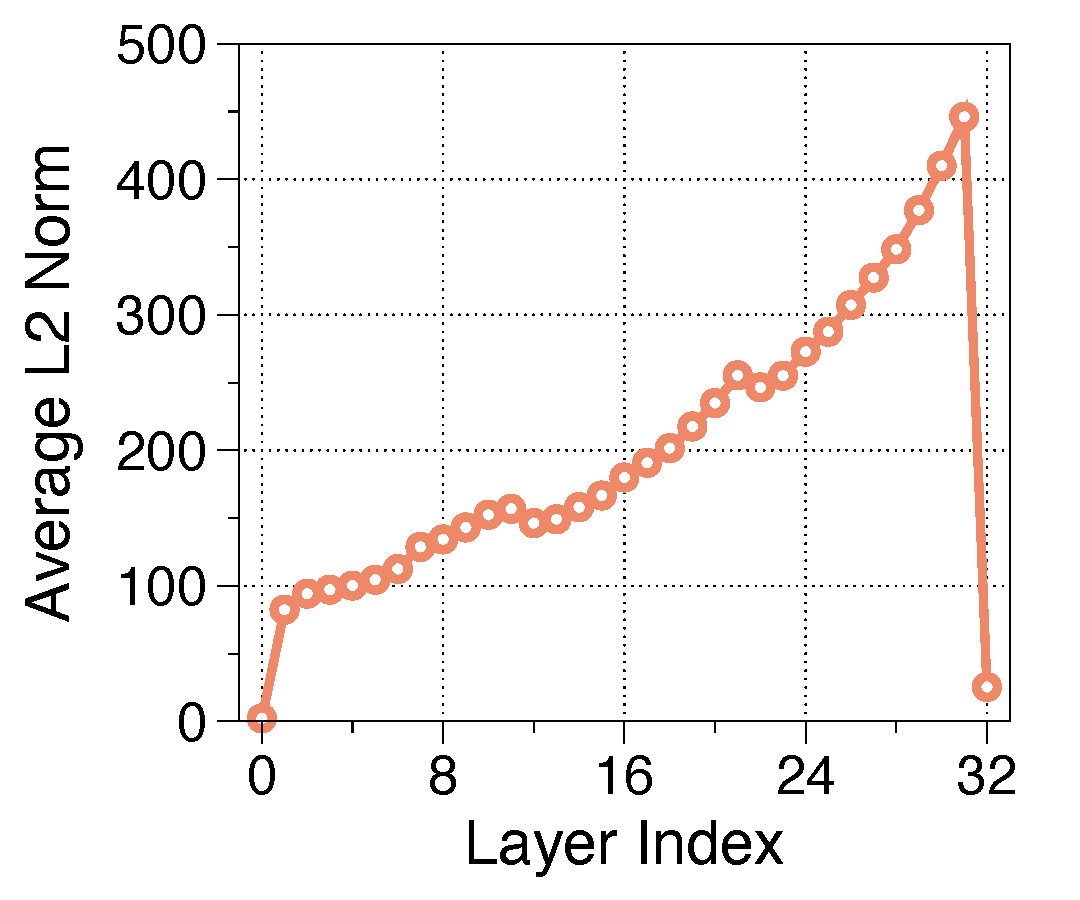
\includegraphics[width=\textwidth]{figs/kv_magnitude/mag_hidden.pdf}
        \subcaption{Hidden states}
    \end{subfigure}
    \centering
    \begin{subfigure}[t]{0.303\textwidth}
    \captionsetup{justification=centering}
        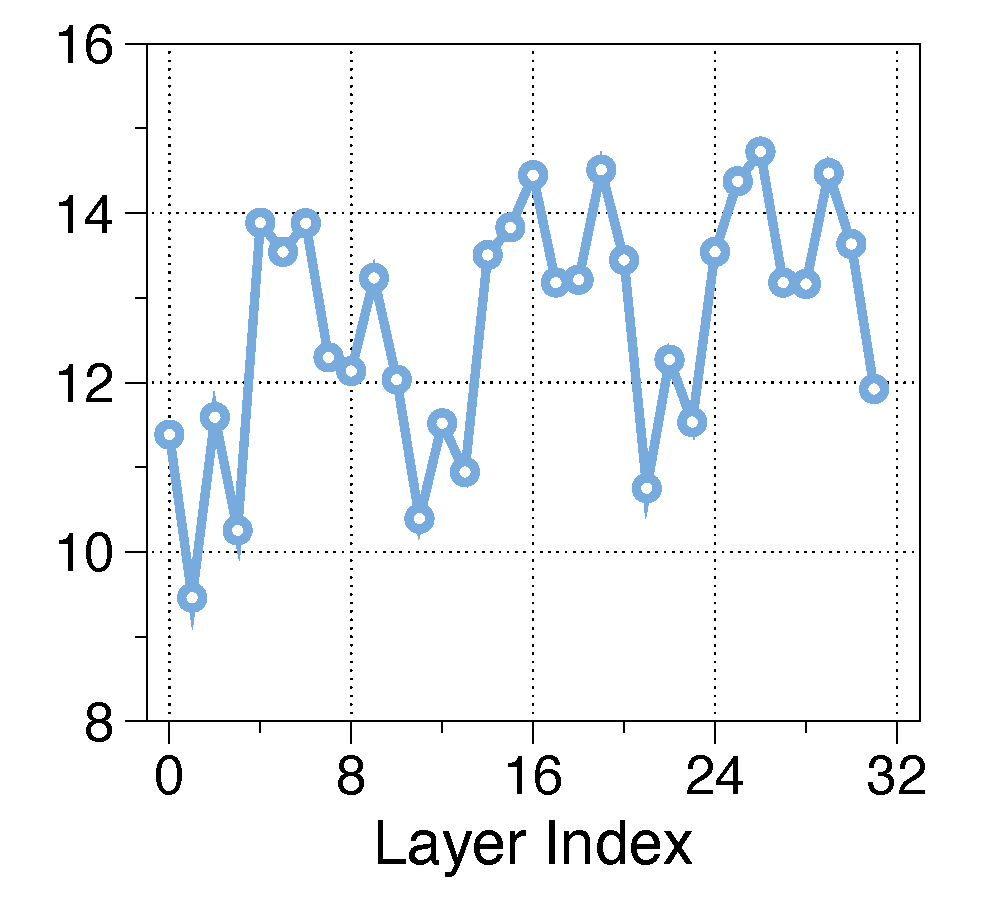
\includegraphics[width=\textwidth]{figs/kv_magnitude/mag_key.pdf}
        \subcaption{Key states}
    \end{subfigure}
    \centering
    \begin{subfigure}[t]{0.303\textwidth}
    \captionsetup{justification=centering}
        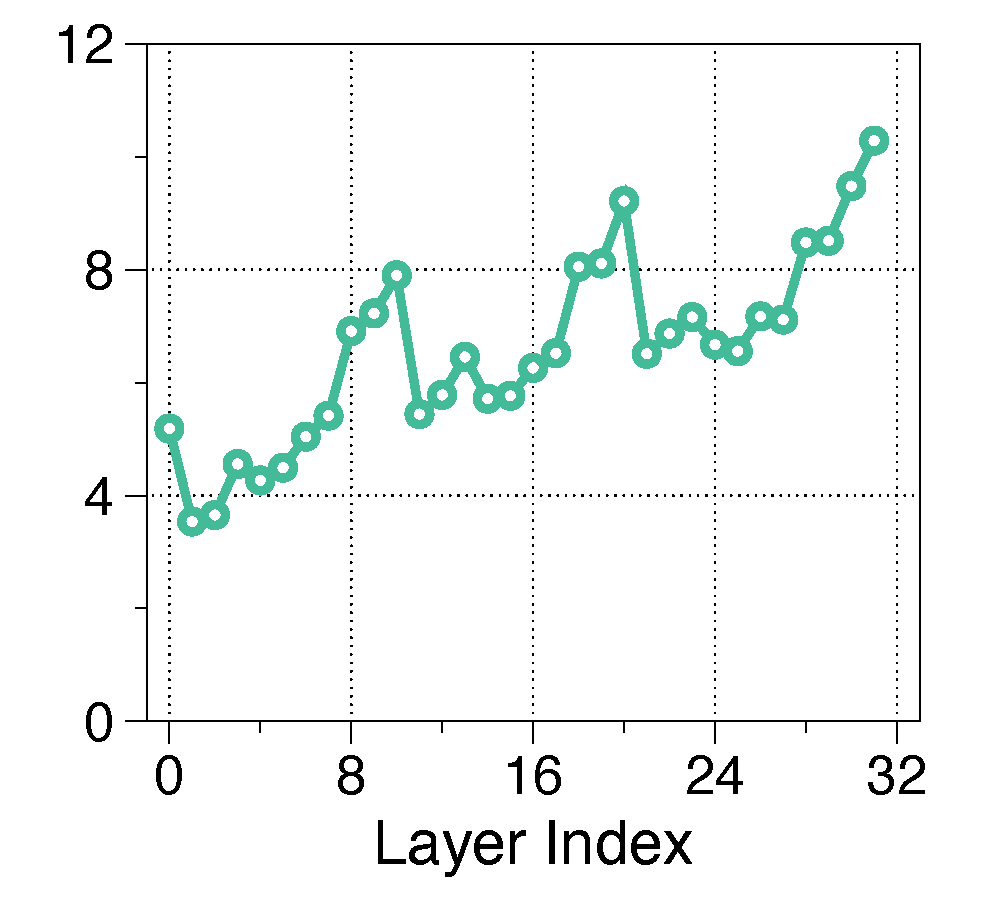
\includegraphics[width=\textwidth]{figs/kv_magnitude/mag_value.pdf}
        \subcaption{Value states}
    \end{subfigure}
    \caption{ Average L2 norm magnitude of (a) hidden states, (b) key states, and (c) value states across layers in a Middle-Cycled Recursive Transformer 360M with 3 recursion steps. 
    Note that the last hidden states correspond to the final hidden states after the last layer normalization. 
    }
    \label{fig:kv_sharing_mag_app}
\end{figure}

When we measured the cosine similarity in \autoref{fig:kv_sharing_dir_app}, distinct diagonal patterns emerge, suggesting that shared projection layers generate highly similar key and value representations. While sharing value states across recursions appears to be more challenging than sharing key states, these findings suggest that the performance drop from KV cache sharing can be marginal even in Recursive Transformers.\looseness=-1



\begin{figure}[h!]
    \centering
    \begin{subfigure}[t]{0.33\textwidth}
    \captionsetup{justification=centering}
        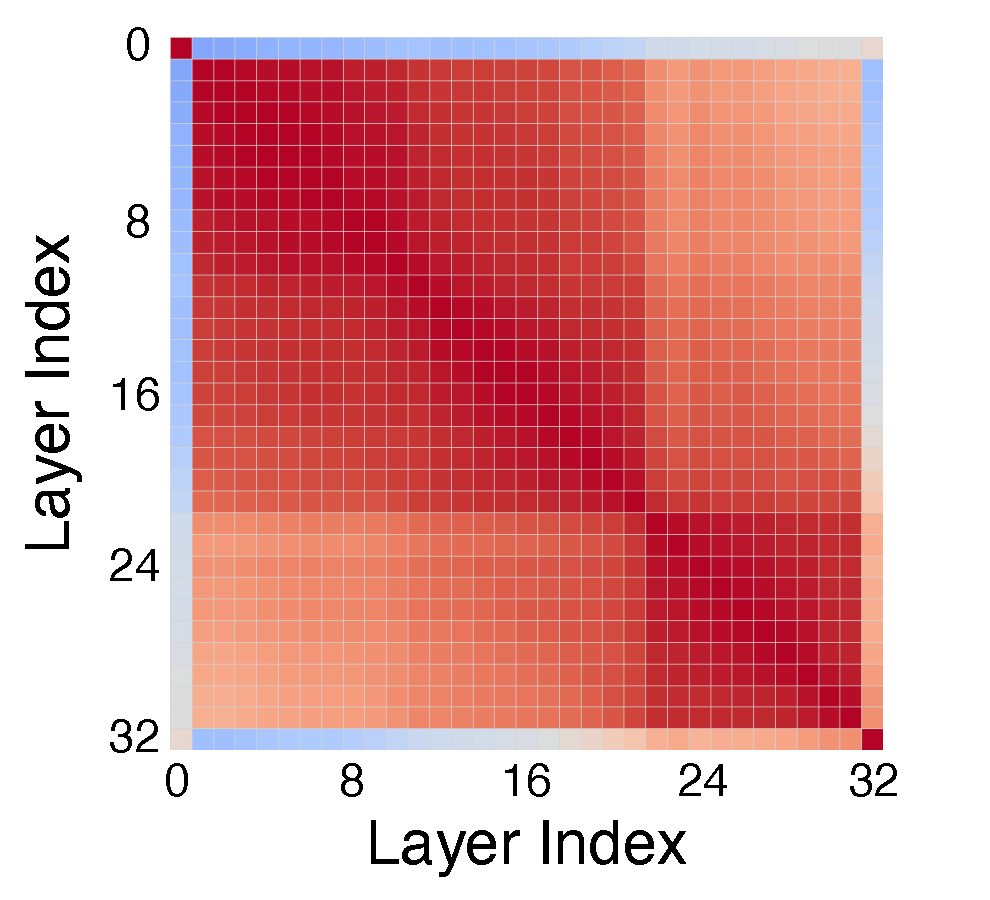
\includegraphics[width=\textwidth]{figs/kv_magnitude/dir_hidden.pdf}
        \subcaption{Hidden states}
    \end{subfigure}
    \centering
    \begin{subfigure}[t]{0.30\textwidth}
    \captionsetup{justification=centering}
        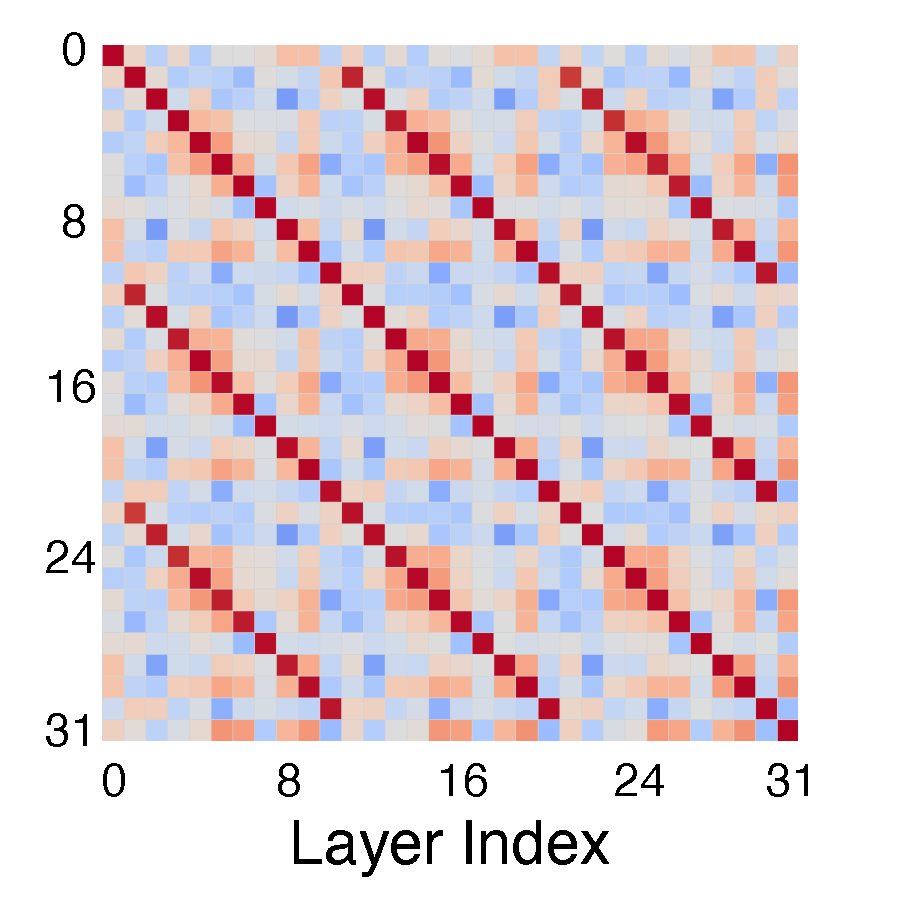
\includegraphics[width=\textwidth]{figs/kv_magnitude/dir_key.pdf}
        \subcaption{Key states}
    \end{subfigure}
    \centering
    \begin{subfigure}[t]{0.33\textwidth}
    \captionsetup{justification=centering}
        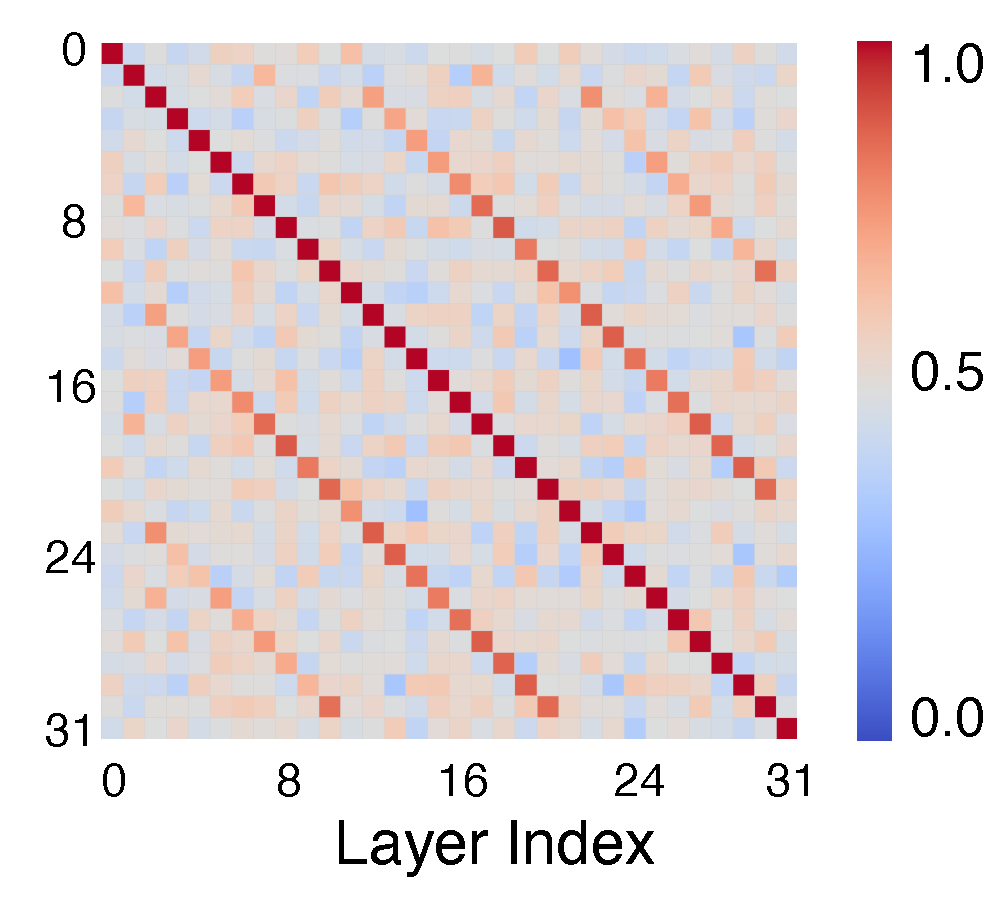
\includegraphics[width=\textwidth]{figs/kv_magnitude/dir_value_cbar.pdf}
        \subcaption{Value states}
    \end{subfigure}
    \caption{ Cosine similarity matrices showing the layer-wise similarity of (a) hidden states, (b) key states, and (c) value states in Recursive Transformer with Middle-Cycle strategy and recursion depth 3. Results are from a 360M parameter model with 32 layers. The hidden states matrix includes the final hidden states after the last layer normalization.
    }
    \label{fig:kv_sharing_dir_app}
\end{figure}


\subsection{Performance Comparison of KV Sharing Strategy}


\paragraph{Experimental results of key-value cache sharing.}
In \autoref{tab:key_value_sharing_results}, we present the performance results when applying KV cache sharing to Vanilla, Recursive, and MoR models. Especially, we tested various strategies for KV caches, including Cycle or Sequence strategies that share the same concepts as parameter sharing (see \S\ref{app:sharing_strategy} for details). Interestingly, KV cache sharing even improves the performance of vanilla models, where sharing acts as a regularization technique.
In case of recursive models, we align the sharing strategy for parameters and KV caches. Despite some variations in the results after applying KV sharing, the Middle-Cycle strategy (the best parameter sharing strategy) showed a slight perplexity drop, albeit not substantial.


When moving to MoR models, they still introduced a small amount of degradation in our best settings (expert-choice router). However, considering the reduced parameter sizes and cache sizes, we believe this minor drop is acceptable. Furthermore, we explored an alternative sharing strategy (indicated by $\dagger$) that utilized shared caches for inactive (unselected) positions while updating active positions through actual computation. This method is analogous to a recursive caching scheme but initializes inactive positions with key-value pairs from the first recursive iteration. Although it did not provide additional benefits, it is still worth exploring combinations of KV sharing and actual updates.\looseness=-1






\begin{table*}[h]
    \caption{
    Comparison of KV cache sharing strategies across Vanilla, Recursive, and MoR Transformers. Models are pretrained on 10B tokens of FineWeb-Edu, and evaluated using negative log-likelihood (NLL) on train set and few-shot accuracy across benchmarks. KV sharing denotes use of recursive KV sharing mechanism. If MoR is mentioned without further specification of KV sharing strategy, it implies the use of the recursion-wise caching strategy. $\text{}^\dagger$It indicates training with hybrid KV sharing that leverages shared caches for inactive positions while updating active ones through actual computation.\looseness=-1
    }
    \label{tab:key_value_sharing_results}
    \small
    \centering
    \resizebox{\textwidth}{!}{
    \setlength{\tabcolsep}{3.5pt}
    \begin{tabular}{l|cc|cc|c|cc|c|cccccc|c}
    \toprule
      &  \multicolumn{2}{c|}{\textbf{Pretrain}} &  \multicolumn{2}{c|}{\textbf{Recursion}} & \textbf{MoR} & \multicolumn{2}{c|}{\textbf{KV Sharing}} & \textbf{NLL\,$\downarrow$} & \multicolumn{7}{c}{\textbf{Few-shot Accuracy\,$\uparrow$}} \\
    \cmidrule(l{2pt}r{2pt}){2-3} \cmidrule(l{2pt}r{2pt}){4-5} \cmidrule(l{2pt}r{2pt}){6-6} \cmidrule(l{2pt}r{2pt}){7-8} \cmidrule(l{2pt}r{2pt}){9-9} \cmidrule(l{2pt}r{2pt}){10-16} 
     \textbf{Models} & N-Emb & $N_L$ & Share & Loop & Type & Share & Loop & FineWeb & LD & HS & PQ & WG & ARC & \!MMLU\! & Avg  \\
    \midrule
    Vanilla & 315M & 32 & - & - & - & - & - & 2.8471 & 27.3 & 34.8 & 64.2 & 52.8 & 38.3 & 26.7 & 40.7\\
    Vanilla & 315M & 32 & - & - & - & Seq & 2 & 2.7848 & 30.0 & 36.5 & 64.6 & 50.7 & 39.4 & 26.9 & 41.3 \\
    \rowcolor[gray]{0.9}
    Vanilla & 315M & 32 & - & - & - & Cyc & 2 & 2.7650 & 30.0 &	36.7 & 65.2 & 51.1  & 39.6 & 27.5 & 41.7\\
    \midrule
    Vanilla & 295M & 30 & - & - & - & - & - & 2.8069 & 29.1 & 35.6 & 65.1 & 50.4 & 38.5 & 27.3 & 41.0 \\
    \rowcolor[gray]{0.9}
    Vanilla & 295M & 30 & - & - & - & Seq & 3 & 2.7879 & 28.3 & 36.4 & 64.3 & 52.7 & 39.4 & 27.3 & 41.4 \\
    Vanilla & 295M & 30 & - & - & - & Cyc & 3 & 2.7890 & 28.9 & 36.5 & 64.6 & 51.4  & 39.0 & 27.6 & 41.3 \\
    \midrule
    Recursive & 157M & 16 & Seq & 2 & - & - & - & 2.9467 & 26.3 & 32.5 & 62.9 & 52.4 & 36.4 & 26.2 & 39.5\\
    Recursive &157M  & 16 & Seq & 2 & - & Seq & 2 & 2.8904 & 26.4 & 33.4 & 64.0 & 51.0 & 37.0 & 26.9 & 39.8\\
    Recursive & 157M & 16 & Cyc & 2 & - & - & - & 2.8487 & 28.5 & 34.8 & 63.1 & 50.0 & 37.4 & 28.8 & 40.1\\
    Recursive & 157M & 16 & Cyc & 2 & - & Cyc & 2 & 2.8577 & 26.2 & 34.5 & 64.2 & 51.4 & 37.3 & 26.9 & 40.1\\
    \rowcolor[gray]{0.9}
    Recursive & 167M & 1+15+1 & M-Cyc & 2 & - & - & - & 2.8295 & 28.6 & 35.0 & 64.5 & 50.5 & 39.7 & 27.2 & 40.9\\
    Recursive & 167M & 1+15+1 & M-Cyc & 2 & - & M-Cyc & 2 & 2.8451 & 27.3 &	34.7 & 63.7 & 50.5 & 37.8 & 27.0 & 40.2 \\
    \midrule
    Recursive & \,\,\,98M & 10 & Seq & 3 & - & - & - & 3.0245 & 24.6 & 31.5 & 63.1 & 49.3 & 35.7 & 25.7 & 38.3\\
    Recursive & \,\,\,98M & 10 & Seq & 3 & - & Seq & 3 & 2.9554 & 24.2 & 32.3 & 62.5 & 52.7 & 36.6 & 26.2 & 39.1\\
    Recursive & \,\,\,98M & 10 & Cyc & 3 & - & - & - & 2.9363 & 25.9 & 33.0 & 62.9 & 50.3 & 36.4 & 26.5 & 39.2\\
    Recursive & \,\,\,98M & 10 & Cyc & 3 & - & Cyc & 3 & 2.9155 & 24.1 & 32.9 & 62.4 & 51.2 & 37.4 & 26.7 & 39.1 \\
    \rowcolor[gray]{0.9}
    Recursive & 118M & 1+10+1 & M-Cyc & 3 & - & - & - & 2.8760 & 28.5 & 34.9 & 64.3 & 50.5 & 39.5 & 27.2 & 40.8\\
    Recursive & 118M & 1+10+1 & M-Cyc & 3 & - & M-Cyc & 3 & 2.8854 & 27.3 &	33.8 & 63.3 & 52.3 & 37.5 & 26.8 &	40.2\\
    \midrule
    \rowcolor[gray]{0.9}
    MoR & 118M & 1+10+1 & M-Cyc & 3 & Expert & - & - & 2.8667 & 27.4 & 34.6 & 63.2 & 51.5 & 37.2 & 26.5 & 40.1\\
    MoR & 118M & 1+10+1 & M-Cyc & 3 & Expert & M-Cyc & 3 & 2.8895 & 34.0 & 	61.6 & 50.2 & 26.0 & 36.5 & 27.0 & 39.2 \\
    MoR & 118M & 1+10+1 & M-Cyc & 3 & Expert & \,\,$\text{M-Cyc}^{\dagger}$ & 3 & 2.8653 & 24.8 & 34.3 & 62.0 & 50.1 & 36.7 & 26.7 & 39.1\\
    \midrule
    \rowcolor[gray]{0.9}
    MoR & 118M & 1+10+1 & M-Cyc & 3 & Token & - & - & 2.9358 & 25.7 & 32.6 & 61.9 & 51.7 & 36.4 & 26.5 & 39.1\\
    MoR & 118M & 1+10+1 & M-Cyc & 3 & Token & M-Cyc & 3 & 2.9155& 25.7 & 32.6 &	61.8 & 49.4 & 36.2 & 26.0 & 38.6\\
    \bottomrule
    \end{tabular}
    }
\end{table*}


\clearpage

\paragraph{Relaxation for key-value sharing constraints.}
We also investigated relaxing the constraints on KV sharing in \autoref{tab:key_value_sharing_relaxation}, similar to the relaxation approach in \citet{bae2024relaxed} for parameter sharing constraints. Specifically, we first re-examined four relaxation techniques for standard Recursive Transformers with very small ranks~\citep{hu2022lora, liu2024dora} or prefix lengths~\citep{liu2021p}. We also experimented with the position encoding~\citep{chen2025inner}, where trainable embeddings are element-wise multiplied with the output of each recursion block. 

Our results show that these techniques do not provide substantial performance improvements when pretraining relaxed models from scratch, consistent with prior studies, as they introduce only a limited number of additional parameters. Although we hypothesize that incorporating prefix-based approaches (such as adding trainable prefixes to attention) into KV sharing might lead to greater benefits, our experiments did not reveal substantial differences in this regard. Further exploration of more sophisticated techniques for efficiently relaxing KV cache sharing constraints remains an open direction for future research.



\begin{table*}[h]
    \caption{
    Experimental results of relaxing parameter sharing and KV cache sharing constraints in Recursive Transformers. All models are trained on FineWeb-Edu with 10B tokens, and we apply the Middle-Cycle parameter sharing for 360M models with 3 recursion depths. We evaluate them based on training NLL and few-shot accuracy across six benchmarks. Relaxation types include encoding trainable embeddings on recursion outputs via element-wise multiplication (Enc), applying LoRA and DoRA to query and value weight matrices, and adaptation prompt tuning (Adapt-P). 
    }
    \label{tab:key_value_sharing_relaxation}
    \small
    \centering
    \resizebox{\textwidth}{!}{
    \setlength{\tabcolsep}{3.5pt}
    \begin{tabular}{l|cc|ccc|cc|c|cccccc|c}
    \toprule
      &  \multicolumn{2}{c|}{\textbf{Pretrain}} &  \multicolumn{3}{c|}{\textbf{Relaxation}} &  \multicolumn{2}{c|}{\textbf{KV Sharing}} & \textbf{NLL\,$\downarrow$} & \multicolumn{7}{c}{\textbf{Few-shot Accuracy\,$\uparrow$}} \\
    \cmidrule(l{2pt}r{2pt}){2-3} \cmidrule(l{2pt}r{2pt}){4-6} \cmidrule(l{2pt}r{2pt}){7-8} \cmidrule(l{2pt}r{2pt}){9-9} \cmidrule(l{2pt}r{2pt}){10-16} 
     \textbf{Models} & N-Emb & $N_L$ & Type & Rank & Len & Share & Loop & FineWeb & LD & HS & PQ & WG & ARC & \!MMLU\! & Avg  \\
    \midrule
    Recursive & 118M & 1+10+1 & - & - & - & - & - & 2.8854 & 27.3 &	33.8 & 63.3 & 52.3 & 37.5 & 26.8 &	40.2\\
    Recursive & 118M & 1+10+1 & Enc & - & - & - & - & 2.8604 & 27.3 & 34.6 & 63.9 & 53.4 & 38.6 & 26.7 & 40.2\\
    Recursive & 124M & 1+10+1 & LoRA & 64 & - & - & - & 2.8599 & 27.3 & 34.6 & 64.3 & 50.9 & 38.0	& 26.9 & 39.7 \\
    Recursive & 124M & 1+10+1 & DoRA & 64 & - & - & - & 2.8945 & 26.4 &	33.6 & 64.4 & 50.6 & 37.4 &	26.5 & 39.2 \\
    Recursive & 126M & 1+10+1 & Adapt-P & - & 256 & - & - & 2.8626 & 27.1 & 34.7 & 64.0 & 51.9	& 37.6 & 26.8 & 39.7\\
    \midrule
    Recursive & 118M & 1+10+1 & - & - & - & M-Cyc & 3 & 2.8854 & 27.3 &	33.8 & 63.3 & 52.3 & 37.5 & 26.8 & 40.2\\
    Recursive & 126M & 1+10+1 & Adapt-P & - & 256 & M-Cyc & 3 & 2.9030 & 24.5 & 33.1 & 63.0 & 52.2 & 26.7 & 37.6 &	39.5\\
    \bottomrule
    \end{tabular}
    }
\end{table*}



\section{Expanded Qualitative Results}
\label{app:qualitative_results}


\subsection{Analysis on Adaptive Computation Paths}


\autoref{tab:qualitative_highlighted_results} illustrates a qualitative analysis of the recursion depth assigned to each subword token. This visualization provides a detailed insight into how tokens within each sample exhibit varying levels of recursive processing, showcasing the adaptive computation mechanism within the MoR framework. Notably, some tokens exit early (purple), while others require deeper processing (blue and red), reflecting the model’s ability to focus more compute on challenging parts of the input.



\begin{table*}[ht]
\centering
\footnotesize
\caption{Visualization of the recursion depth for each subword token, with colors representing the number of recursion steps: \raisebox{0pt}[0.5em][0.1em]{\colorbox{DarkOrchid!25}{1}}, \raisebox{0pt}[0.5em][0.1em]{\colorbox{SkyBlue!55}{2}}, and \raisebox{0pt}[0.5em][0.1em]{\colorbox{Salmon!60}{3}}. This depth specifically indicates how many times recursion is applied at that token's position to predict the subsequent token. Each row corresponds to a single sample, offering a clear illustration of the token-level recursion distribution in practice. We use an MoR model with $N_r = 3$, auxiliary loss, and recursion-wise KV caching. This model is built on a 360M parameter base and trained on 30B tokens.
}
\begin{tabular}{@{}l p{13cm}@{}}
\toprule
\textbf{Sample} & \textbf{Text} \\
\midrule

\vspace{10pt}
Sample \#1 &
{\setlength{\fboxsep}{1pt}\raisebox{0pt}[0.5em][0.1em]{\colorbox{Salmon!60}{\strut{People}}}}{\setlength{\fboxsep}{1pt}\raisebox{0pt}[0.5em][0.1em]{\colorbox{DarkOrchid!25}{\strut{ who}}}}{\setlength{\fboxsep}{1pt}\raisebox{0pt}[0.5em][0.1em]{\colorbox{DarkOrchid!25}{\strut{ feel}}}}{\setlength{\fboxsep}{1pt}\raisebox{0pt}[0.5em][0.1em]{\colorbox{DarkOrchid!25}{\strut{ comfortable}}}}{\setlength{\fboxsep}{1pt}\raisebox{0pt}[0.5em][0.1em]{\colorbox{DarkOrchid!25}{\strut{ defending}}}}{\setlength{\fboxsep}{1pt}\raisebox{0pt}[0.5em][0.1em]{\colorbox{DarkOrchid!25}{\strut{ their}}}}{\setlength{\fboxsep}{1pt}\raisebox{0pt}[0.5em][0.1em]{\colorbox{DarkOrchid!25}{\strut{ views}}}}{\setlength{\fboxsep}{1pt}\raisebox{0pt}[0.5em][0.1em]{\colorbox{SkyBlue!55}{\strut{—}}}}{\setlength{\fboxsep}{1pt}\raisebox{0pt}[0.5em][0.1em]{\colorbox{DarkOrchid!25}{\strut{def}}}}{\setlength{\fboxsep}{1pt}\raisebox{0pt}[0.5em][0.1em]{\colorbox{Salmon!60}{\strut{ensively}}}}{\setlength{\fboxsep}{1pt}\raisebox{0pt}[0.5em][0.1em]{\colorbox{Salmon!60}{\strut{ confident}}}}{\setlength{\fboxsep}{1pt}\raisebox{0pt}[0.5em][0.1em]{\colorbox{SkyBlue!55}{\strut{—}}}}{\setlength{\fboxsep}{1pt}\raisebox{0pt}[0.5em][0.1em]{\colorbox{DarkOrchid!25}{\strut{may}}}}{\setlength{\fboxsep}{1pt}\raisebox{0pt}[0.5em][0.1em]{\colorbox{DarkOrchid!25}{\strut{ also}}}}{\setlength{\fboxsep}{1pt}\raisebox{0pt}[0.5em][0.1em]{\colorbox{Salmon!60}{\strut{ eventually}}}} {\setlength{\fboxsep}{1pt}\raisebox{0pt}[0.5em][0.1em]{\colorbox{DarkOrchid!25}{\strut{ change}}}}{\setlength{\fboxsep}{1pt}\raisebox{0pt}[0.5em][0.1em]{\colorbox{SkyBlue!55}{\strut{ those}}}}{\setlength{\fboxsep}{1pt}\raisebox{0pt}[0.5em][0.1em]{\colorbox{DarkOrchid!25}{\strut{ views}}}}{\setlength{\fboxsep}{1pt}\raisebox{0pt}[0.5em][0.1em]{\colorbox{SkyBlue!55}{\strut{ and}}}}{\setlength{\fboxsep}{1pt}\raisebox{0pt}[0.5em][0.1em]{\colorbox{Salmon!60}{\strut{ corresponding}}}}{\setlength{\fboxsep}{1pt}\raisebox{0pt}[0.5em][0.1em]{\colorbox{DarkOrchid!25}{\strut{ behaviors}}}}{\setlength{\fboxsep}{1pt}\raisebox{0pt}[0.5em][0.1em]{\colorbox{DarkOrchid!25}{\strut{.}}}}{\setlength{\fboxsep}{1pt}\raisebox{0pt}[0.5em][0.1em]{\colorbox{SkyBlue!55}{\strut{ National}}}}{\setlength{\fboxsep}{1pt}\raisebox{0pt}[0.5em][0.1em]{\colorbox{Salmon!60}{\strut{ Election}}}}{\setlength{\fboxsep}{1pt}\raisebox{0pt}[0.5em][0.1em]{\colorbox{Salmon!60}{\strut{ Studies}}}}{\setlength{\fboxsep}{1pt}\raisebox{0pt}[0.5em][0.1em]{\colorbox{Salmon!60}{\strut{ surveys}}}}{\setlength{\fboxsep}{1pt}\raisebox{0pt}[0.5em][0.1em]{\colorbox{DarkOrchid!25}{\strut{ showed}}}}{\setlength{\fboxsep}{1pt}\raisebox{0pt}[0.5em][0.1em]{\colorbox{DarkOrchid!25}{\strut{ that}}}} {\setlength{\fboxsep}{1pt}\raisebox{0pt}[0.5em][0.1em]{\colorbox{SkyBlue!55}{\strut{ defensive}}}}{\setlength{\fboxsep}{1pt}\raisebox{0pt}[0.5em][0.1em]{\colorbox{Salmon!60}{\strut{ confidence}}}}{\setlength{\fboxsep}{1pt}\raisebox{0pt}[0.5em][0.1em]{\colorbox{SkyBlue!55}{\strut{ predicted}}}}{\setlength{\fboxsep}{1pt}\raisebox{0pt}[0.5em][0.1em]{\colorbox{DarkOrchid!25}{\strut{ def}}}}{\setlength{\fboxsep}{1pt}\raisebox{0pt}[0.5em][0.1em]{\colorbox{Salmon!60}{\strut{ection}}}}{\setlength{\fboxsep}{1pt}\raisebox{0pt}[0.5em][0.1em]{\colorbox{SkyBlue!55}{\strut{ in}}}}{\setlength{\fboxsep}{1pt}\raisebox{0pt}[0.5em][0.1em]{\colorbox{SkyBlue!55}{\strut{ the}}}}{\setlength{\fboxsep}{1pt}\raisebox{0pt}[0.5em][0.1em]{\colorbox{DarkOrchid!25}{\strut{ }}}}{\setlength{\fboxsep}{1pt}\raisebox{0pt}[0.5em][0.1em]{\colorbox{SkyBlue!55}{\strut{2}}}}{\setlength{\fboxsep}{1pt}\raisebox{0pt}[0.5em][0.1em]{\colorbox{DarkOrchid!25}{\strut{0}}}}{\setlength{\fboxsep}{1pt}\raisebox{0pt}[0.5em][0.1em]{\colorbox{SkyBlue!55}{\strut{0}}}}{\setlength{\fboxsep}{1pt}\raisebox{0pt}[0.5em][0.1em]{\colorbox{Salmon!60}{\strut{6}}}}{\setlength{\fboxsep}{1pt}\raisebox{0pt}[0.5em][0.1em]{\colorbox{DarkOrchid!25}{\strut{ U}}}}{\setlength{\fboxsep}{1pt}\raisebox{0pt}[0.5em][0.1em]{\colorbox{DarkOrchid!25}{\strut{.}}}}{\setlength{\fboxsep}{1pt}\raisebox{0pt}[0.5em][0.1em]{\colorbox{DarkOrchid!25}{\strut{S}}}}{\setlength{\fboxsep}{1pt}\raisebox{0pt}[0.5em][0.1em]{\colorbox{Salmon!60}{\strut{.}}}}{\setlength{\fboxsep}{1pt}\raisebox{0pt}[0.5em][0.1em]{\colorbox{Salmon!60}{\strut{ House}}}}{\setlength{\fboxsep}{1pt}\raisebox{0pt}[0.5em][0.1em]{\colorbox{DarkOrchid!25}{\strut{ elections}}}}{\setlength{\fboxsep}{1pt}\raisebox{0pt}[0.5em][0.1em]{\colorbox{SkyBlue!55}{\strut{,}}}}{\setlength{\fboxsep}{1pt}\raisebox{0pt}[0.5em][0.1em]{\colorbox{Salmon!60}{\strut{ above}}}}{\setlength{\fboxsep}{1pt}\raisebox{0pt}[0.5em][0.1em]{\colorbox{SkyBlue!55}{\strut{ and}}}}{\setlength{\fboxsep}{1pt}\raisebox{0pt}[0.5em][0.1em]{\colorbox{SkyBlue!55}{\strut{ beyond}}}} 
{\setlength{\fboxsep}{1pt}\raisebox{0pt}[0.5em][0.1em]{\colorbox{SkyBlue!55}{\strut{ the}}}}{\setlength{\fboxsep}{1pt}\raisebox{0pt}[0.5em][0.1em]{\colorbox{Salmon!60}{\strut{ impact}}}}{\setlength{\fboxsep}{1pt}\raisebox{0pt}[0.5em][0.1em]{\colorbox{SkyBlue!55}{\strut{ of}}}}{\setlength{\fboxsep}{1pt}\raisebox{0pt}[0.5em][0.1em]{\colorbox{Salmon!60}{\strut{ various}}}}{\setlength{\fboxsep}{1pt}\raisebox{0pt}[0.5em][0.1em]{\colorbox{Salmon!60}{\strut{ demographic}}}}{\setlength{\fboxsep}{1pt}\raisebox{0pt}[0.5em][0.1em]{\colorbox{SkyBlue!55}{\strut{ and}}}}{\setlength{\fboxsep}{1pt}\raisebox{0pt}[0.5em][0.1em]{\colorbox{Salmon!60}{\strut{ political}}}}{\setlength{\fboxsep}{1pt}\raisebox{0pt}[0.5em][0.1em]{\colorbox{DarkOrchid!25}{\strut{ variables}}}}{\setlength{\fboxsep}{1pt}\raisebox{0pt}[0.5em][0.1em]{\colorbox{DarkOrchid!25}{\strut{.}}}}{\setlength{\fboxsep}{1pt}\raisebox{0pt}[0.5em][0.1em]{\colorbox{DarkOrchid!25}{\strut{ Moreover}}}}{\setlength{\fboxsep}{1pt}\raisebox{0pt}[0.5em][0.1em]{\colorbox{DarkOrchid!25}{\strut{,}}}}{\setlength{\fboxsep}{1pt}\raisebox{0pt}[0.5em][0.1em]{\colorbox{SkyBlue!55}{\strut{ defensive}}}}{\setlength{\fboxsep}{1pt}\raisebox{0pt}[0.5em][0.1em]{\colorbox{Salmon!60}{\strut{ confidence}}}}{\setlength{\fboxsep}{1pt}\raisebox{0pt}[0.5em][0.1em]{\colorbox{SkyBlue!55}{\strut{ was}}}}
{\setlength{\fboxsep}{1pt}\raisebox{0pt}[0.5em][0.1em]{\colorbox{Salmon!60}{\strut{ also}}}}{\setlength{\fboxsep}{1pt}\raisebox{0pt}[0.5em][0.1em]{\colorbox{DarkOrchid!25}{\strut{ associated}}}}{\setlength{\fboxsep}{1pt}\raisebox{0pt}[0.5em][0.1em]{\colorbox{SkyBlue!55}{\strut{ with}}}}{\setlength{\fboxsep}{1pt}\raisebox{0pt}[0.5em][0.1em]{\colorbox{Salmon!60}{\strut{ political}}}}{\setlength{\fboxsep}{1pt}\raisebox{0pt}[0.5em][0.1em]{\colorbox{Salmon!60}{\strut{ knowledge}}}}{\setlength{\fboxsep}{1pt}\raisebox{0pt}[0.5em][0.1em]{\colorbox{SkyBlue!55}{\strut{ and}}}}{\setlength{\fboxsep}{1pt}\raisebox{0pt}[0.5em][0.1em]{\colorbox{Salmon!60}{\strut{ attention}}}}{\setlength{\fboxsep}{1pt}\raisebox{0pt}[0.5em][0.1em]{\colorbox{Salmon!60}{\strut{ to}}}}{\setlength{\fboxsep}{1pt}\raisebox{0pt}[0.5em][0.1em]{\colorbox{Salmon!60}{\strut{ politics}}}}{\setlength{\fboxsep}{1pt}\raisebox{0pt}[0.5em][0.1em]{\colorbox{SkyBlue!55}{\strut{ and}}}}{\setlength{\fboxsep}{1pt}\raisebox{0pt}[0.5em][0.1em]{\colorbox{Salmon!60}{\strut{ government}}}}{\setlength{\fboxsep}{1pt}\raisebox{0pt}[0.5em][0.1em]{\colorbox{DarkOrchid!25}{\strut{ affairs}}}}{\setlength{\fboxsep}{1pt}\raisebox{0pt}[0.5em][0.1em]{\colorbox{SkyBlue!55}{\strut{,}}}}{\setlength{\fboxsep}{1pt}\raisebox{0pt}[0.5em][0.1em]{\colorbox{SkyBlue!55}{\strut{ but}}}}{\setlength{\fboxsep}{1pt}\raisebox{0pt}[0.5em][0.1em]{\colorbox{Salmon!60}{\strut{ not}}}}\\


\vspace{10pt}
Sample \#2 &
{\setlength{\fboxsep}{1pt}\raisebox{0pt}[0.5em][0.1em]{\colorbox{Salmon!60}{\strut{2}}}}{\setlength{\fboxsep}{1pt}\raisebox{0pt}[0.5em][0.1em]{\colorbox{DarkOrchid!25}{\strut{0}}}}{\setlength{\fboxsep}{1pt}\raisebox{0pt}[0.5em][0.1em]{\colorbox{DarkOrchid!25}{\strut{1}}}}{\setlength{\fboxsep}{1pt}\raisebox{0pt}[0.5em][0.1em]{\colorbox{DarkOrchid!25}{\strut{4}}}}{\setlength{\fboxsep}{1pt}\raisebox{0pt}[0.5em][0.1em]{\colorbox{DarkOrchid!25}{\strut{,}}}}{\setlength{\fboxsep}{1pt}\raisebox{0pt}[0.5em][0.1em]{\colorbox{DarkOrchid!25}{\strut{ }}}}{\setlength{\fboxsep}{1pt}\raisebox{0pt}[0.5em][0.1em]{\colorbox{DarkOrchid!25}{\strut{7}}}}{\setlength{\fboxsep}{1pt}\raisebox{0pt}[0.5em][0.1em]{\colorbox{DarkOrchid!25}{\strut{:}}}}{\setlength{\fboxsep}{1pt}\raisebox{0pt}[0.5em][0.1em]{\colorbox{DarkOrchid!25}{\strut{5}}}}{\setlength{\fboxsep}{1pt}\raisebox{0pt}[0.5em][0.1em]{\colorbox{DarkOrchid!25}{\strut{7}}}}{\setlength{\fboxsep}{1pt}\raisebox{0pt}[0.5em][0.1em]{\colorbox{DarkOrchid!25}{\strut{ AM}}}}{\setlength{\fboxsep}{1pt}\raisebox{0pt}[0.5em][0.1em]{\colorbox{DarkOrchid!25}{\strut{ }}}}{\setlength{\fboxsep}{1pt}\raisebox{0pt}[0.5em][0.1em]{\colorbox{DarkOrchid!25}{\strut{Space}}}}{\setlength{\fboxsep}{1pt}\raisebox{0pt}[0.5em][0.1em]{\colorbox{Salmon!60}{\strut{X}}}}{\setlength{\fboxsep}{1pt}\raisebox{0pt}[0.5em][0.1em]{\colorbox{DarkOrchid!25}{\strut{ Falcon}}}}{\setlength{\fboxsep}{1pt}\raisebox{0pt}[0.5em][0.1em]{\colorbox{DarkOrchid!25}{\strut{ }}}}{\setlength{\fboxsep}{1pt}\raisebox{0pt}[0.5em][0.1em]{\colorbox{Salmon!60}{\strut{9}}}}{\setlength{\fboxsep}{1pt}\raisebox{0pt}[0.5em][0.1em]{\colorbox{SkyBlue!55}{\strut{-}}}}{\setlength{\fboxsep}{1pt}\raisebox{0pt}[0.5em][0.1em]{\colorbox{SkyBlue!55}{\strut{R}}}}{\setlength{\fboxsep}{1pt}\raisebox{0pt}[0.5em][0.1em]{\colorbox{Salmon!60}{\strut{ Rocket}}}}{\setlength{\fboxsep}{1pt}\raisebox{0pt}[0.5em][0.1em]{\colorbox{DarkOrchid!25}{\strut{ Suff}}}}{\setlength{\fboxsep}{1pt}\raisebox{0pt}[0.5em][0.1em]{\colorbox{SkyBlue!55}{\strut{ers}}}}{\setlength{\fboxsep}{1pt}\raisebox{0pt}[0.5em][0.1em]{\colorbox{DarkOrchid!25}{\strut{ M}}}}{\setlength{\fboxsep}{1pt}\raisebox{0pt}[0.5em][0.1em]{\colorbox{DarkOrchid!25}{\strut{alf}}}}{\setlength{\fboxsep}{1pt}\raisebox{0pt}[0.5em][0.1em]{\colorbox{Salmon!60}{\strut{unction}}}}{\setlength{\fboxsep}{1pt}\raisebox{0pt}[0.5em][0.1em]{\colorbox{SkyBlue!55}{\strut{,}}}}{\setlength{\fboxsep}{1pt}\raisebox{0pt}[0.5em][0.1em]{\colorbox{Salmon!60}{\strut{ Self}}}}{\setlength{\fboxsep}{1pt}\raisebox{0pt}[0.5em][0.1em]{\colorbox{DarkOrchid!25}{\strut{-}}}}{\setlength{\fboxsep}{1pt}\raisebox{0pt}[0.5em][0.1em]{\colorbox{DarkOrchid!25}{\strut{Dest}}}}{\setlength{\fboxsep}{1pt}\raisebox{0pt}[0.5em][0.1em]{\colorbox{Salmon!60}{\strut{ruct}}}}{\setlength{\fboxsep}{1pt}\raisebox{0pt}[0.5em][0.1em]{\colorbox{Salmon!60}{\strut{s}}}}{\setlength{\fboxsep}{1pt}\raisebox{0pt}[0.5em][0.1em]{\colorbox{SkyBlue!55}{\strut{ During}}}}

{\setlength{\fboxsep}{1pt}\raisebox{0pt}[0.5em][0.1em]{\colorbox{Salmon!60}{\strut{ Test}}}}{\setlength{\fboxsep}{1pt}\raisebox{0pt}[0.5em][0.1em]{\colorbox{Salmon!60}{\strut{ Flight}}}}{\setlength{\fboxsep}{1pt}\raisebox{0pt}[0.5em][0.1em]{\colorbox{DarkOrchid!25}{\strut{ }}}}{\setlength{\fboxsep}{1pt}\raisebox{0pt}[0.5em][0.1em]{\colorbox{DarkOrchid!25}{\strut{August}}}}{\setlength{\fboxsep}{1pt}\raisebox{0pt}[0.5em][0.1em]{\colorbox{DarkOrchid!25}{\strut{ }}}}{\setlength{\fboxsep}{1pt}\raisebox{0pt}[0.5em][0.1em]{\colorbox{DarkOrchid!25}{\strut{2}}}}{\setlength{\fboxsep}{1pt}\raisebox{0pt}[0.5em][0.1em]{\colorbox{DarkOrchid!25}{\strut{3}}}}{\setlength{\fboxsep}{1pt}\raisebox{0pt}[0.5em][0.1em]{\colorbox{DarkOrchid!25}{\strut{,}}}}{\setlength{\fboxsep}{1pt}\raisebox{0pt}[0.5em][0.1em]{\colorbox{DarkOrchid!25}{\strut{ }}}}{\setlength{\fboxsep}{1pt}\raisebox{0pt}[0.5em][0.1em]{\colorbox{DarkOrchid!25}{\strut{2}}}}{\setlength{\fboxsep}{1pt}\raisebox{0pt}[0.5em][0.1em]{\colorbox{DarkOrchid!25}{\strut{0}}}}{\setlength{\fboxsep}{1pt}\raisebox{0pt}[0.5em][0.1em]{\colorbox{DarkOrchid!25}{\strut{1}}}}{\setlength{\fboxsep}{1pt}\raisebox{0pt}[0.5em][0.1em]{\colorbox{DarkOrchid!25}{\strut{4}}}}{\setlength{\fboxsep}{1pt}\raisebox{0pt}[0.5em][0.1em]{\colorbox{DarkOrchid!25}{\strut{,}}}}{\setlength{\fboxsep}{1pt}\raisebox{0pt}[0.5em][0.1em]{\colorbox{DarkOrchid!25}{\strut{ }}}}{\setlength{\fboxsep}{1pt}\raisebox{0pt}[0.5em][0.1em]{\colorbox{SkyBlue!55}{\strut{9}}}}{\setlength{\fboxsep}{1pt}\raisebox{0pt}[0.5em][0.1em]{\colorbox{DarkOrchid!25}{\strut{:}}}}{\setlength{\fboxsep}{1pt}\raisebox{0pt}[0.5em][0.1em]{\colorbox{SkyBlue!55}{\strut{3}}}}{\setlength{\fboxsep}{1pt}\raisebox{0pt}[0.5em][0.1em]{\colorbox{Salmon!60}{\strut{6}}}}{\setlength{\fboxsep}{1pt}\raisebox{0pt}[0.5em][0.1em]{\colorbox{DarkOrchid!25}{\strut{ AM}}}}{\setlength{\fboxsep}{1pt}\raisebox{0pt}[0.5em][0.1em]{\colorbox{DarkOrchid!25}{\strut{ }}}}{\setlength{\fboxsep}{1pt}\raisebox{0pt}[0.5em][0.1em]{\colorbox{SkyBlue!55}{\strut{Texas}}}}{\setlength{\fboxsep}{1pt}\raisebox{0pt}[0.5em][0.1em]{\colorbox{DarkOrchid!25}{\strut{ Ch}}}}{\setlength{\fboxsep}{1pt}\raisebox{0pt}[0.5em][0.1em]{\colorbox{Salmon!60}{\strut{osen}}}}{\setlength{\fboxsep}{1pt}\raisebox{0pt}[0.5em][0.1em]{\colorbox{SkyBlue!55}{\strut{ as}}}}{\setlength{\fboxsep}{1pt}\raisebox{0pt}[0.5em][0.1em]{\colorbox{Salmon!60}{\strut{ Site}}}}{\setlength{\fboxsep}{1pt}\raisebox{0pt}[0.5em][0.1em]{\colorbox{SkyBlue!55}{\strut{ for}}}}{\setlength{\fboxsep}{1pt}\raisebox{0pt}[0.5em][0.1em]{\colorbox{Salmon!60}{\strut{ SpaceX}}}}{\setlength{\fboxsep}{1pt}\raisebox{0pt}[0.5em][0.1em]{\colorbox{SkyBlue!55}{\strut{\&\#x27;s}}}}{\setlength{\fboxsep}{1pt}\raisebox{0pt}[0.5em][0.1em]{\colorbox{Salmon!60}{\strut{ First}}}}

{\setlength{\fboxsep}{1pt}\raisebox{0pt}[0.5em][0.1em]{\colorbox{Salmon!60}{\strut{ Commercial}}}}{\setlength{\fboxsep}{1pt}\raisebox{0pt}[0.5em][0.1em]{\colorbox{Salmon!60}{\strut{ Launch}}}}{\setlength{\fboxsep}{1pt}\raisebox{0pt}[0.5em][0.1em]{\colorbox{Salmon!60}{\strut{pad}}}}{\setlength{\fboxsep}{1pt}\raisebox{0pt}[0.5em][0.1em]{\colorbox{DarkOrchid!25}{\strut{ }}}}{\setlength{\fboxsep}{1pt}\raisebox{0pt}[0.5em][0.1em]{\colorbox{DarkOrchid!25}{\strut{August}}}}{\setlength{\fboxsep}{1pt}\raisebox{0pt}[0.5em][0.1em]{\colorbox{DarkOrchid!25}{\strut{ }}}}{\setlength{\fboxsep}{1pt}\raisebox{0pt}[0.5em][0.1em]{\colorbox{SkyBlue!55}{\strut{5}}}}{\setlength{\fboxsep}{1pt}\raisebox{0pt}[0.5em][0.1em]{\colorbox{DarkOrchid!25}{\strut{,}}}}{\setlength{\fboxsep}{1pt}\raisebox{0pt}[0.5em][0.1em]{\colorbox{DarkOrchid!25}{\strut{ }}}}{\setlength{\fboxsep}{1pt}\raisebox{0pt}[0.5em][0.1em]{\colorbox{DarkOrchid!25}{\strut{2}}}}{\setlength{\fboxsep}{1pt}\raisebox{0pt}[0.5em][0.1em]{\colorbox{DarkOrchid!25}{\strut{0}}}}{\setlength{\fboxsep}{1pt}\raisebox{0pt}[0.5em][0.1em]{\colorbox{DarkOrchid!25}{\strut{1}}}}{\setlength{\fboxsep}{1pt}\raisebox{0pt}[0.5em][0.1em]{\colorbox{DarkOrchid!25}{\strut{4}}}}{\setlength{\fboxsep}{1pt}\raisebox{0pt}[0.5em][0.1em]{\colorbox{DarkOrchid!25}{\strut{,}}}}{\setlength{\fboxsep}{1pt}\raisebox{0pt}[0.5em][0.1em]{\colorbox{DarkOrchid!25}{\strut{ }}}}{\setlength{\fboxsep}{1pt}\raisebox{0pt}[0.5em][0.1em]{\colorbox{SkyBlue!55}{\strut{1}}}}{\setlength{\fboxsep}{1pt}\raisebox{0pt}[0.5em][0.1em]{\colorbox{DarkOrchid!25}{\strut{:}}}}{\setlength{\fboxsep}{1pt}\raisebox{0pt}[0.5em][0.1em]{\colorbox{SkyBlue!55}{\strut{4}}}}{\setlength{\fboxsep}{1pt}\raisebox{0pt}[0.5em][0.1em]{\colorbox{Salmon!60}{\strut{4}}}}{\setlength{\fboxsep}{1pt}\raisebox{0pt}[0.5em][0.1em]{\colorbox{DarkOrchid!25}{\strut{ PM}}}}{\setlength{\fboxsep}{1pt}\raisebox{0pt}[0.5em][0.1em]{\colorbox{DarkOrchid!25}{\strut{ }}}}{\setlength{\fboxsep}{1pt}\raisebox{0pt}[0.5em][0.1em]{\colorbox{SkyBlue!55}{\strut{South}}}}{\setlength{\fboxsep}{1pt}\raisebox{0pt}[0.5em][0.1em]{\colorbox{SkyBlue!55}{\strut{ Carolina}}}}{\setlength{\fboxsep}{1pt}\raisebox{0pt}[0.5em][0.1em]{\colorbox{Salmon!60}{\strut{ Prison}}}}{\setlength{\fboxsep}{1pt}\raisebox{0pt}[0.5em][0.1em]{\colorbox{Salmon!60}{\strut{ Find}}}}{\setlength{\fboxsep}{1pt}\raisebox{0pt}[0.5em][0.1em]{\colorbox{SkyBlue!55}{\strut{s}}}}{\setlength{\fboxsep}{1pt}\raisebox{0pt}[0.5em][0.1em]{\colorbox{DarkOrchid!25}{\strut{ C}}}}{\setlength{\fboxsep}{1pt}\raisebox{0pt}[0.5em][0.1em]{\colorbox{DarkOrchid!25}{\strut{ras}}}}{\setlength{\fboxsep}{1pt}\raisebox{0pt}[0.5em][0.1em]{\colorbox{Salmon!60}{\strut{hed}}}}

{\setlength{\fboxsep}{1pt}\raisebox{0pt}[0.5em][0.1em]{\colorbox{DarkOrchid!25}{\strut{ Dr}}}}{\setlength{\fboxsep}{1pt}\raisebox{0pt}[0.5em][0.1em]{\colorbox{Salmon!60}{\strut{one}}}}{\setlength{\fboxsep}{1pt}\raisebox{0pt}[0.5em][0.1em]{\colorbox{Salmon!60}{\strut{ Car}}}}{\setlength{\fboxsep}{1pt}\raisebox{0pt}[0.5em][0.1em]{\colorbox{Salmon!60}{\strut{rying}}}}{\setlength{\fboxsep}{1pt}\raisebox{0pt}[0.5em][0.1em]{\colorbox{Salmon!60}{\strut{ Drugs}}}}{\setlength{\fboxsep}{1pt}\raisebox{0pt}[0.5em][0.1em]{\colorbox{SkyBlue!55}{\strut{,}}}}{\setlength{\fboxsep}{1pt}\raisebox{0pt}[0.5em][0.1em]{\colorbox{DarkOrchid!25}{\strut{ Ph}}}}{\setlength{\fboxsep}{1pt}\raisebox{0pt}[0.5em][0.1em]{\colorbox{Salmon!60}{\strut{ones}}}}{\setlength{\fboxsep}{1pt}\raisebox{0pt}[0.5em][0.1em]{\colorbox{DarkOrchid!25}{\strut{ }}}}{\setlength{\fboxsep}{1pt}\raisebox{0pt}[0.5em][0.1em]{\colorbox{DarkOrchid!25}{\strut{August}}}}{\setlength{\fboxsep}{1pt}\raisebox{0pt}[0.5em][0.1em]{\colorbox{SkyBlue!55}{\strut{ }}}}{\setlength{\fboxsep}{1pt}\raisebox{0pt}[0.5em][0.1em]{\colorbox{SkyBlue!55}{\strut{1}}}}{\setlength{\fboxsep}{1pt}\raisebox{0pt}[0.5em][0.1em]{\colorbox{DarkOrchid!25}{\strut{,}}}}{\setlength{\fboxsep}{1pt}\raisebox{0pt}[0.5em][0.1em]{\colorbox{DarkOrchid!25}{\strut{ }}}}{\setlength{\fboxsep}{1pt}\raisebox{0pt}[0.5em][0.1em]{\colorbox{DarkOrchid!25}{\strut{2}}}}{\setlength{\fboxsep}{1pt}\raisebox{0pt}[0.5em][0.1em]{\colorbox{DarkOrchid!25}{\strut{0}}}}{\setlength{\fboxsep}{1pt}\raisebox{0pt}[0.5em][0.1em]{\colorbox{DarkOrchid!25}{\strut{1}}}}{\setlength{\fboxsep}{1pt}\raisebox{0pt}[0.5em][0.1em]{\colorbox{Salmon!60}{\strut{4}}}}{\setlength{\fboxsep}{1pt}\raisebox{0pt}[0.5em][0.1em]{\colorbox{DarkOrchid!25}{\strut{,}}}}{\setlength{\fboxsep}{1pt}\raisebox{0pt}[0.5em][0.1em]{\colorbox{DarkOrchid!25}{\strut{ }}}}{\setlength{\fboxsep}{1pt}\raisebox{0pt}[0.5em][0.1em]{\colorbox{SkyBlue!55}{\strut{2}}}}{\setlength{\fboxsep}{1pt}\raisebox{0pt}[0.5em][0.1em]{\colorbox{DarkOrchid!25}{\strut{:}}}}{\setlength{\fboxsep}{1pt}\raisebox{0pt}[0.5em][0.1em]{\colorbox{SkyBlue!55}{\strut{4}}}}{\setlength{\fboxsep}{1pt}\raisebox{0pt}[0.5em][0.1em]{\colorbox{Salmon!60}{\strut{9}}}}{\setlength{\fboxsep}{1pt}\raisebox{0pt}[0.5em][0.1em]{\colorbox{DarkOrchid!25}{\strut{ PM}}}}{\setlength{\fboxsep}{1pt}\raisebox{0pt}[0.5em][0.1em]{\colorbox{DarkOrchid!25}{\strut{ }}}}{\setlength{\fboxsep}{1pt}\raisebox{0pt}[0.5em][0.1em]{\colorbox{SkyBlue!55}{\strut{NASA}}}}{\setlength{\fboxsep}{1pt}\raisebox{0pt}[0.5em][0.1em]{\colorbox{SkyBlue!55}{\strut{\&\#x27;s}}}}{\setlength{\fboxsep}{1pt}\raisebox{0pt}[0.5em][0.1em]{\colorbox{SkyBlue!55}{\strut{ Mars}}}}{\setlength{\fboxsep}{1pt}\raisebox{0pt}[0.5em][0.1em]{\colorbox{DarkOrchid!25}{\strut{ }}}}{\setlength{\fboxsep}{1pt}\raisebox{0pt}[0.5em][0.1em]{\colorbox{SkyBlue!55}{\strut{2}}}}{\setlength{\fboxsep}{1pt}\raisebox{0pt}[0.5em][0.1em]{\colorbox{Salmon!60}{\strut{0}}}}{\setlength{\fboxsep}{1pt}\raisebox{0pt}[0.5em][0.1em]{\colorbox{SkyBlue!55}{\strut{2}}}}{\setlength{\fboxsep}{1pt}\raisebox{0pt}[0.5em][0.1em]{\colorbox{Salmon!60}{\strut{0}}}}

{\setlength{\fboxsep}{1pt}\raisebox{0pt}[0.5em][0.1em]{\colorbox{Salmon!60}{\strut{ Rover}}}}{\setlength{\fboxsep}{1pt}\raisebox{0pt}[0.5em][0.1em]{\colorbox{DarkOrchid!25}{\strut{ G}}}}{\setlength{\fboxsep}{1pt}\raisebox{0pt}[0.5em][0.1em]{\colorbox{Salmon!60}{\strut{ains}}}}{\setlength{\fboxsep}{1pt}\raisebox{0pt}[0.5em][0.1em]{\colorbox{Salmon!60}{\strut{ Seven}}}}{\setlength{\fboxsep}{1pt}\raisebox{0pt}[0.5em][0.1em]{\colorbox{Salmon!60}{\strut{ New}}}}{\setlength{\fboxsep}{1pt}\raisebox{0pt}[0.5em][0.1em]{\colorbox{Salmon!60}{\strut{ Instruments}}}}{\setlength{\fboxsep}{1pt}\raisebox{0pt}[0.5em][0.1em]{\colorbox{SkyBlue!55}{\strut{ for}}}}{\setlength{\fboxsep}{1pt}\raisebox{0pt}[0.5em][0.1em]{\colorbox{Salmon!60}{\strut{ Exploration}}}}{\setlength{\fboxsep}{1pt}\raisebox{0pt}[0.5em][0.1em]{\colorbox{DarkOrchid!25}{\strut{ }}}}{\setlength{\fboxsep}{1pt}\raisebox{0pt}[0.5em][0.1em]{\colorbox{DarkOrchid!25}{\strut{August}}}}{\setlength{\fboxsep}{1pt}\raisebox{0pt}[0.5em][0.1em]{\colorbox{SkyBlue!55}{\strut{ }}}}{\setlength{\fboxsep}{1pt}\raisebox{0pt}[0.5em][0.1em]{\colorbox{SkyBlue!55}{\strut{1}}}}{\setlength{\fboxsep}{1pt}\raisebox{0pt}[0.5em][0.1em]{\colorbox{DarkOrchid!25}{\strut{,}}}}{\setlength{\fboxsep}{1pt}\raisebox{0pt}[0.5em][0.1em]{\colorbox{DarkOrchid!25}{\strut{ }}}}{\setlength{\fboxsep}{1pt}\raisebox{0pt}[0.5em][0.1em]{\colorbox{DarkOrchid!25}{\strut{2}}}}{\setlength{\fboxsep}{1pt}\raisebox{0pt}[0.5em][0.1em]{\colorbox{DarkOrchid!25}{\strut{0}}}}{\setlength{\fboxsep}{1pt}\raisebox{0pt}[0.5em][0.1em]{\colorbox{DarkOrchid!25}{\strut{1}}}}{\setlength{\fboxsep}{1pt}\raisebox{0pt}[0.5em][0.1em]{\colorbox{Salmon!60}{\strut{4}}}}{\setlength{\fboxsep}{1pt}\raisebox{0pt}[0.5em][0.1em]{\colorbox{DarkOrchid!25}{\strut{,}}}}{\setlength{\fboxsep}{1pt}\raisebox{0pt}[0.5em][0.1em]{\colorbox{Salmon!60}{\strut{ }}}}{\setlength{\fboxsep}{1pt}\raisebox{0pt}[0.5em][0.1em]{\colorbox{SkyBlue!55}{\strut{1}}}}{\setlength{\fboxsep}{1pt}\raisebox{0pt}[0.5em][0.1em]{\colorbox{SkyBlue!55}{\strut{:}}}}{\setlength{\fboxsep}{1pt}\raisebox{0pt}[0.5em][0.1em]{\colorbox{SkyBlue!55}{\strut{3}}}}{\setlength{\fboxsep}{1pt}\raisebox{0pt}[0.5em][0.1em]{\colorbox{Salmon!60}{\strut{0}}}}{\setlength{\fboxsep}{1pt}\raisebox{0pt}[0.5em][0.1em]{\colorbox{DarkOrchid!25}{\strut{ PM}}}}{\setlength{\fboxsep}{1pt}\raisebox{0pt}[0.5em][0.1em]{\colorbox{DarkOrchid!25}{\strut{ }}}}{\setlength{\fboxsep}{1pt}\raisebox{0pt}[0.5em][0.1em]{\colorbox{SkyBlue!55}{\strut{NASA}}}} \\


\vspace{10pt}
Sample \#3 &
{\setlength{\fboxsep}{1pt}\raisebox{0pt}[0.5em][0.1em]{\colorbox{Salmon!60}{\strut{9}}}}{\setlength{\fboxsep}{1pt}\raisebox{0pt}[0.5em][0.1em]{\colorbox{DarkOrchid!25}{\strut{ PR}}}}{\setlength{\fboxsep}{1pt}\raisebox{0pt}[0.5em][0.1em]{\colorbox{DarkOrchid!25}{\strut{ New}}}}{\setlength{\fboxsep}{1pt}\raisebox{0pt}[0.5em][0.1em]{\colorbox{DarkOrchid!25}{\strut{sw}}}}{\setlength{\fboxsep}{1pt}\raisebox{0pt}[0.5em][0.1em]{\colorbox{Salmon!60}{\strut{ire}}}}{\setlength{\fboxsep}{1pt}\raisebox{0pt}[0.5em][0.1em]{\colorbox{DarkOrchid!25}{\strut{.}}}}{\setlength{\fboxsep}{1pt}\raisebox{0pt}[0.5em][0.1em]{\colorbox{DarkOrchid!25}{\strut{ }}}}{\setlength{\fboxsep}{1pt}\raisebox{0pt}[0.5em][0.1em]{\colorbox{DarkOrchid!25}{\strut{All}}}}{\setlength{\fboxsep}{1pt}\raisebox{0pt}[0.5em][0.1em]{\colorbox{DarkOrchid!25}{\strut{ rights}}}}{\setlength{\fboxsep}{1pt}\raisebox{0pt}[0.5em][0.1em]{\colorbox{DarkOrchid!25}{\strut{ reserved}}}}{\setlength{\fboxsep}{1pt}\raisebox{0pt}[0.5em][0.1em]{\colorbox{DarkOrchid!25}{\strut{}}}}{\setlength{\fboxsep}{1pt}\raisebox{0pt}[0.5em][0.1em]{\colorbox{DarkOrchid!25}{\strut{A}}}}{\setlength{\fboxsep}{1pt}\raisebox{0pt}[0.5em][0.1em]{\colorbox{DarkOrchid!25}{\strut{ report}}}}{\setlength{\fboxsep}{1pt}\raisebox{0pt}[0.5em][0.1em]{\colorbox{DarkOrchid!25}{\strut{ released}}}}{\setlength{\fboxsep}{1pt}\raisebox{0pt}[0.5em][0.1em]{\colorbox{DarkOrchid!25}{\strut{ Thursday}}}}{\setlength{\fboxsep}{1pt}\raisebox{0pt}[0.5em][0.1em]{\colorbox{SkyBlue!55}{\strut{ on}}}}{\setlength{\fboxsep}{1pt}\raisebox{0pt}[0.5em][0.1em]{\colorbox{SkyBlue!55}{\strut{ the}}}}{\setlength{\fboxsep}{1pt}\raisebox{0pt}[0.5em][0.1em]{\colorbox{Salmon!60}{\strut{ Slide}}}}{\setlength{\fboxsep}{1pt}\raisebox{0pt}[0.5em][0.1em]{\colorbox{Salmon!60}{\strut{ Fire}}}}{\setlength{\fboxsep}{1pt}\raisebox{0pt}[0.5em][0.1em]{\colorbox{SkyBlue!55}{\strut{ in}}}}{\setlength{\fboxsep}{1pt}\raisebox{0pt}[0.5em][0.1em]{\colorbox{SkyBlue!55}{\strut{ Oak}}}}{\setlength{\fboxsep}{1pt}\raisebox{0pt}[0.5em][0.1em]{\colorbox{Salmon!60}{\strut{ Creek}}}}

{\setlength{\fboxsep}{1pt}\raisebox{0pt}[0.5em][0.1em]{\colorbox{Salmon!60}{\strut{ Canyon}}}}{\setlength{\fboxsep}{1pt}\raisebox{0pt}[0.5em][0.1em]{\colorbox{DarkOrchid!25}{\strut{ doesn}}}}{\setlength{\fboxsep}{1pt}\raisebox{0pt}[0.5em][0.1em]{\colorbox{Salmon!60}{\strut{\&\#x27;t}}}}{\setlength{\fboxsep}{1pt}\raisebox{0pt}[0.5em][0.1em]{\colorbox{Salmon!60}{\strut{ hold}}}}{\setlength{\fboxsep}{1pt}\raisebox{0pt}[0.5em][0.1em]{\colorbox{Salmon!60}{\strut{ back}}}}{\setlength{\fboxsep}{1pt}\raisebox{0pt}[0.5em][0.1em]{\colorbox{Salmon!60}{\strut{ in}}}}{\setlength{\fboxsep}{1pt}\raisebox{0pt}[0.5em][0.1em]{\colorbox{Salmon!60}{\strut{ laying}}}}{\setlength{\fboxsep}{1pt}\raisebox{0pt}[0.5em][0.1em]{\colorbox{Salmon!60}{\strut{ out}}}}{\setlength{\fboxsep}{1pt}\raisebox{0pt}[0.5em][0.1em]{\colorbox{SkyBlue!55}{\strut{ the}}}}{\setlength{\fboxsep}{1pt}\raisebox{0pt}[0.5em][0.1em]{\colorbox{DarkOrchid!25}{\strut{ danger}}}}{\setlength{\fboxsep}{1pt}\raisebox{0pt}[0.5em][0.1em]{\colorbox{SkyBlue!55}{\strut{ facing}}}}{\setlength{\fboxsep}{1pt}\raisebox{0pt}[0.5em][0.1em]{\colorbox{SkyBlue!55}{\strut{ the}}}}{\setlength{\fboxsep}{1pt}\raisebox{0pt}[0.5em][0.1em]{\colorbox{Salmon!60}{\strut{ burned}}}}{\setlength{\fboxsep}{1pt}\raisebox{0pt}[0.5em][0.1em]{\colorbox{DarkOrchid!25}{\strut{-}}}}{\setlength{\fboxsep}{1pt}\raisebox{0pt}[0.5em][0.1em]{\colorbox{Salmon!60}{\strut{out}}}}{\setlength{\fboxsep}{1pt}\raisebox{0pt}[0.5em][0.1em]{\colorbox{Salmon!60}{\strut{ area}}}}{\setlength{\fboxsep}{1pt}\raisebox{0pt}[0.5em][0.1em]{\colorbox{DarkOrchid!25}{\strut{.}}}}{\setlength{\fboxsep}{1pt}\raisebox{0pt}[0.5em][0.1em]{\colorbox{DarkOrchid!25}{\strut{ }}}}{\setlength{\fboxsep}{1pt}\raisebox{0pt}[0.5em][0.1em]{\colorbox{DarkOrchid!25}{\strut{The}}}}{\setlength{\fboxsep}{1pt}\raisebox{0pt}[0.5em][0.1em]{\colorbox{DarkOrchid!25}{\strut{ U}}}}{\setlength{\fboxsep}{1pt}\raisebox{0pt}[0.5em][0.1em]{\colorbox{DarkOrchid!25}{\strut{.}}}}

{\setlength{\fboxsep}{1pt}\raisebox{0pt}[0.5em][0.1em]{\colorbox{DarkOrchid!25}{\strut{S}}}}{\setlength{\fboxsep}{1pt}\raisebox{0pt}[0.5em][0.1em]{\colorbox{SkyBlue!55}{\strut{.}}}}{\setlength{\fboxsep}{1pt}\raisebox{0pt}[0.5em][0.1em]{\colorbox{SkyBlue!55}{\strut{ Forest}}}}{\setlength{\fboxsep}{1pt}\raisebox{0pt}[0.5em][0.1em]{\colorbox{Salmon!60}{\strut{ Service}}}}{\setlength{\fboxsep}{1pt}\raisebox{0pt}[0.5em][0.1em]{\colorbox{SkyBlue!55}{\strut{ issued}}}}{\setlength{\fboxsep}{1pt}\raisebox{0pt}[0.5em][0.1em]{\colorbox{SkyBlue!55}{\strut{ the}}}}{\setlength{\fboxsep}{1pt}\raisebox{0pt}[0.5em][0.1em]{\colorbox{Salmon!60}{\strut{ report}}}}{\setlength{\fboxsep}{1pt}\raisebox{0pt}[0.5em][0.1em]{\colorbox{DarkOrchid!25}{\strut{ Thursday}}}}{\setlength{\fboxsep}{1pt}\raisebox{0pt}[0.5em][0.1em]{\colorbox{DarkOrchid!25}{\strut{ afternoon}}}}{\setlength{\fboxsep}{1pt}\raisebox{0pt}[0.5em][0.1em]{\colorbox{SkyBlue!55}{\strut{ stating}}}}{\setlength{\fboxsep}{1pt}\raisebox{0pt}[0.5em][0.1em]{\colorbox{SkyBlue!55}{\strut{ the}}}}{\setlength{\fboxsep}{1pt}\raisebox{0pt}[0.5em][0.1em]{\colorbox{Salmon!60}{\strut{ biggest}}}}{\setlength{\fboxsep}{1pt}\raisebox{0pt}[0.5em][0.1em]{\colorbox{DarkOrchid!25}{\strut{ concern}}}}{\setlength{\fboxsep}{1pt}\raisebox{0pt}[0.5em][0.1em]{\colorbox{SkyBlue!55}{\strut{ is}}}}{\setlength{\fboxsep}{1pt}\raisebox{0pt}[0.5em][0.1em]{\colorbox{SkyBlue!55}{\strut{ the}}}}{\setlength{\fboxsep}{1pt}\raisebox{0pt}[0.5em][0.1em]{\colorbox{DarkOrchid!25}{\strut{ st}}}}{\setlength{\fboxsep}{1pt}\raisebox{0pt}[0.5em][0.1em]{\colorbox{Salmon!60}{\strut{eeper}}}}

{\setlength{\fboxsep}{1pt}\raisebox{0pt}[0.5em][0.1em]{\colorbox{Salmon!60}{\strut{ slopes}}}}{\setlength{\fboxsep}{1pt}\raisebox{0pt}[0.5em][0.1em]{\colorbox{SkyBlue!55}{\strut{ of}}}}{\setlength{\fboxsep}{1pt}\raisebox{0pt}[0.5em][0.1em]{\colorbox{SkyBlue!55}{\strut{ Oak}}}}{\setlength{\fboxsep}{1pt}\raisebox{0pt}[0.5em][0.1em]{\colorbox{Salmon!60}{\strut{ Creek}}}}{\setlength{\fboxsep}{1pt}\raisebox{0pt}[0.5em][0.1em]{\colorbox{Salmon!60}{\strut{ Canyon}}}}{\setlength{\fboxsep}{1pt}\raisebox{0pt}[0.5em][0.1em]{\colorbox{Salmon!60}{\strut{ is}}}}{\setlength{\fboxsep}{1pt}\raisebox{0pt}[0.5em][0.1em]{\colorbox{Salmon!60}{\strut{ especially}}}}{\setlength{\fboxsep}{1pt}\raisebox{0pt}[0.5em][0.1em]{\colorbox{DarkOrchid!25}{\strut{ subject}}}}{\setlength{\fboxsep}{1pt}\raisebox{0pt}[0.5em][0.1em]{\colorbox{SkyBlue!55}{\strut{ to}}}}{\setlength{\fboxsep}{1pt}\raisebox{0pt}[0.5em][0.1em]{\colorbox{Salmon!60}{\strut{ debris}}}}{\setlength{\fboxsep}{1pt}\raisebox{0pt}[0.5em][0.1em]{\colorbox{Salmon!60}{\strut{ flows}}}}{\setlength{\fboxsep}{1pt}\raisebox{0pt}[0.5em][0.1em]{\colorbox{Salmon!60}{\strut{,}}}}{\setlength{\fboxsep}{1pt}\raisebox{0pt}[0.5em][0.1em]{\colorbox{Salmon!60}{\strut{ rocks}}}}{\setlength{\fboxsep}{1pt}\raisebox{0pt}[0.5em][0.1em]{\colorbox{DarkOrchid!25}{\strut{l}}}}{\setlength{\fboxsep}{1pt}\raisebox{0pt}[0.5em][0.1em]{\colorbox{DarkOrchid!25}{\strut{ides}}}}{\setlength{\fboxsep}{1pt}\raisebox{0pt}[0.5em][0.1em]{\colorbox{SkyBlue!55}{\strut{,}}}}{\setlength{\fboxsep}{1pt}\raisebox{0pt}[0.5em][0.1em]{\colorbox{Salmon!60}{\strut{ flash}}}}{\setlength{\fboxsep}{1pt}\raisebox{0pt}[0.5em][0.1em]{\colorbox{DarkOrchid!25}{\strut{ flooding}}}}{\setlength{\fboxsep}{1pt}\raisebox{0pt}[0.5em][0.1em]{\colorbox{SkyBlue!55}{\strut{ and}}}}

{\setlength{\fboxsep}{1pt}\raisebox{0pt}[0.5em][0.1em]{\colorbox{DarkOrchid!25}{\strut{ erosion}}}}{\setlength{\fboxsep}{1pt}\raisebox{0pt}[0.5em][0.1em]{\colorbox{Salmon!60}{\strut{ that}}}}{\setlength{\fboxsep}{1pt}\raisebox{0pt}[0.5em][0.1em]{\colorbox{Salmon!60}{\strut{ could}}}}{\setlength{\fboxsep}{1pt}\raisebox{0pt}[0.5em][0.1em]{\colorbox{SkyBlue!55}{\strut{ become}}}}{\setlength{\fboxsep}{1pt}\raisebox{0pt}[0.5em][0.1em]{\colorbox{Salmon!60}{\strut{ concentrated}}}}{\setlength{\fboxsep}{1pt}\raisebox{0pt}[0.5em][0.1em]{\colorbox{Salmon!60}{\strut{ flow}}}}{\setlength{\fboxsep}{1pt}\raisebox{0pt}[0.5em][0.1em]{\colorbox{SkyBlue!55}{\strut{ or}}}}{\setlength{\fboxsep}{1pt}\raisebox{0pt}[0.5em][0.1em]{\colorbox{SkyBlue!55}{\strut{ a}}}}{\setlength{\fboxsep}{1pt}\raisebox{0pt}[0.5em][0.1em]{\colorbox{Salmon!60}{\strut{ landslide}}}}{\setlength{\fboxsep}{1pt}\raisebox{0pt}[0.5em][0.1em]{\colorbox{DarkOrchid!25}{\strut{.}}}}{\setlength{\fboxsep}{1pt}\raisebox{0pt}[0.5em][0.1em]{\colorbox{DarkOrchid!25}{\strut{ }}}}{\setlength{\fboxsep}{1pt}\raisebox{0pt}[0.5em][0.1em]{\colorbox{DarkOrchid!25}{\strut{The}}}}{\setlength{\fboxsep}{1pt}\raisebox{0pt}[0.5em][0.1em]{\colorbox{DarkOrchid!25}{\strut{ report}}}}{\setlength{\fboxsep}{1pt}\raisebox{0pt}[0.5em][0.1em]{\colorbox{SkyBlue!55}{\strut{ said}}}}{\setlength{\fboxsep}{1pt}\raisebox{0pt}[0.5em][0.1em]{\colorbox{SkyBlue!55}{\strut{ in}}}}{\setlength{\fboxsep}{1pt}\raisebox{0pt}[0.5em][0.1em]{\colorbox{Salmon!60}{\strut{ smaller}}}}{\setlength{\fboxsep}{1pt}\raisebox{0pt}[0.5em][0.1em]{\colorbox{Salmon!60}{\strut{ streams}}}}\\


\vspace{10pt}
Sample \#4 &
{\setlength{\fboxsep}{1pt}\raisebox{0pt}[0.5em][0.1em]{\colorbox{Salmon!60}{\strut{ Bil}}}}{\setlength{\fboxsep}{1pt}\raisebox{0pt}[0.5em][0.1em]{\colorbox{DarkOrchid!25}{\strut{bo}}}}{\setlength{\fboxsep}{1pt}\raisebox{0pt}[0.5em][0.1em]{\colorbox{DarkOrchid!25}{\strut{ to}}}}{\setlength{\fboxsep}{1pt}\raisebox{0pt}[0.5em][0.1em]{\colorbox{DarkOrchid!25}{\strut{ accompany}}}}{\setlength{\fboxsep}{1pt}\raisebox{0pt}[0.5em][0.1em]{\colorbox{DarkOrchid!25}{\strut{ the}}}}{\setlength{\fboxsep}{1pt}\raisebox{0pt}[0.5em][0.1em]{\colorbox{DarkOrchid!25}{\strut{ dwar}}}}{\setlength{\fboxsep}{1pt}\raisebox{0pt}[0.5em][0.1em]{\colorbox{DarkOrchid!25}{\strut{ves}}}}{\setlength{\fboxsep}{1pt}\raisebox{0pt}[0.5em][0.1em]{\colorbox{Salmon!60}{\strut{ to}}}}{\setlength{\fboxsep}{1pt}\raisebox{0pt}[0.5em][0.1em]{\colorbox{Salmon!60}{\strut{ fight}}}}{\setlength{\fboxsep}{1pt}\raisebox{0pt}[0.5em][0.1em]{\colorbox{SkyBlue!55}{\strut{ the}}}}{\setlength{\fboxsep}{1pt}\raisebox{0pt}[0.5em][0.1em]{\colorbox{DarkOrchid!25}{\strut{ enemy}}}}{\setlength{\fboxsep}{1pt}\raisebox{0pt}[0.5em][0.1em]{\colorbox{DarkOrchid!25}{\strut{.}}}}{\setlength{\fboxsep}{1pt}\raisebox{0pt}[0.5em][0.1em]{\colorbox{DarkOrchid!25}{\strut{ He}}}}{\setlength{\fboxsep}{1pt}\raisebox{0pt}[0.5em][0.1em]{\colorbox{DarkOrchid!25}{\strut{ says}}}}{\setlength{\fboxsep}{1pt}\raisebox{0pt}[0.5em][0.1em]{\colorbox{DarkOrchid!25}{\strut{,}}}}{\setlength{\fboxsep}{1pt}\raisebox{0pt}[0.5em][0.1em]{\colorbox{DarkOrchid!25}{\strut{ “}}}}{\setlength{\fboxsep}{1pt}\raisebox{0pt}[0.5em][0.1em]{\colorbox{DarkOrchid!25}{\strut{S}}}}{\setlength{\fboxsep}{1pt}\raisebox{0pt}[0.5em][0.1em]{\colorbox{SkyBlue!55}{\strut{ar}}}}{\setlength{\fboxsep}{1pt}\raisebox{0pt}[0.5em][0.1em]{\colorbox{Salmon!60}{\strut{uman}}}}{\setlength{\fboxsep}{1pt}\raisebox{0pt}[0.5em][0.1em]{\colorbox{SkyBlue!55}{\strut{ believes}}}}{\setlength{\fboxsep}{1pt}\raisebox{0pt}[0.5em][0.1em]{\colorbox{Salmon!60}{\strut{ it}}}}{\setlength{\fboxsep}{1pt}\raisebox{0pt}[0.5em][0.1em]{\colorbox{SkyBlue!55}{\strut{ is}}}}{\setlength{\fboxsep}{1pt}\raisebox{0pt}[0.5em][0.1em]{\colorbox{Salmon!60}{\strut{ only}}}}

{\setlength{\fboxsep}{1pt}\raisebox{0pt}[0.5em][0.1em]{\colorbox{Salmon!60}{\strut{ great}}}}{\setlength{\fboxsep}{1pt}\raisebox{0pt}[0.5em][0.1em]{\colorbox{Salmon!60}{\strut{ power}}}}{\setlength{\fboxsep}{1pt}\raisebox{0pt}[0.5em][0.1em]{\colorbox{Salmon!60}{\strut{ that}}}}{\setlength{\fboxsep}{1pt}\raisebox{0pt}[0.5em][0.1em]{\colorbox{Salmon!60}{\strut{ can}}}}{\setlength{\fboxsep}{1pt}\raisebox{0pt}[0.5em][0.1em]{\colorbox{Salmon!60}{\strut{ hold}}}}{\setlength{\fboxsep}{1pt}\raisebox{0pt}[0.5em][0.1em]{\colorbox{Salmon!60}{\strut{ evil}}}}{\setlength{\fboxsep}{1pt}\raisebox{0pt}[0.5em][0.1em]{\colorbox{SkyBlue!55}{\strut{ in}}}}{\setlength{\fboxsep}{1pt}\raisebox{0pt}[0.5em][0.1em]{\colorbox{DarkOrchid!25}{\strut{ check}}}}{\setlength{\fboxsep}{1pt}\raisebox{0pt}[0.5em][0.1em]{\colorbox{Salmon!60}{\strut{,}}}}{\setlength{\fboxsep}{1pt}\raisebox{0pt}[0.5em][0.1em]{\colorbox{SkyBlue!55}{\strut{ but}}}}{\setlength{\fboxsep}{1pt}\raisebox{0pt}[0.5em][0.1em]{\colorbox{SkyBlue!55}{\strut{ that}}}}{\setlength{\fboxsep}{1pt}\raisebox{0pt}[0.5em][0.1em]{\colorbox{SkyBlue!55}{\strut{ is}}}}{\setlength{\fboxsep}{1pt}\raisebox{0pt}[0.5em][0.1em]{\colorbox{Salmon!60}{\strut{ not}}}}{\setlength{\fboxsep}{1pt}\raisebox{0pt}[0.5em][0.1em]{\colorbox{SkyBlue!55}{\strut{ what}}}}{\setlength{\fboxsep}{1pt}\raisebox{0pt}[0.5em][0.1em]{\colorbox{Salmon!60}{\strut{ I}}}}{\setlength{\fboxsep}{1pt}\raisebox{0pt}[0.5em][0.1em]{\colorbox{Salmon!60}{\strut{ have}}}}{\setlength{\fboxsep}{1pt}\raisebox{0pt}[0.5em][0.1em]{\colorbox{Salmon!60}{\strut{ found}}}}{\setlength{\fboxsep}{1pt}\raisebox{0pt}[0.5em][0.1em]{\colorbox{DarkOrchid!25}{\strut{.}}}}{\setlength{\fboxsep}{1pt}\raisebox{0pt}[0.5em][0.1em]{\colorbox{DarkOrchid!25}{\strut{ I}}}}{\setlength{\fboxsep}{1pt}\raisebox{0pt}[0.5em][0.1em]{\colorbox{SkyBlue!55}{\strut{ found}}}}{\setlength{\fboxsep}{1pt}\raisebox{0pt}[0.5em][0.1em]{\colorbox{Salmon!60}{\strut{ it}}}}{\setlength{\fboxsep}{1pt}\raisebox{0pt}[0.5em][0.1em]{\colorbox{SkyBlue!55}{\strut{ is}}}}{\setlength{\fboxsep}{1pt}\raisebox{0pt}[0.5em][0.1em]{\colorbox{SkyBlue!55}{\strut{ the}}}}

{\setlength{\fboxsep}{1pt}\raisebox{0pt}[0.5em][0.1em]{\colorbox{Salmon!60}{\strut{ small}}}}{\setlength{\fboxsep}{1pt}\raisebox{0pt}[0.5em][0.1em]{\colorbox{Salmon!60}{\strut{ everyday}}}}{\setlength{\fboxsep}{1pt}\raisebox{0pt}[0.5em][0.1em]{\colorbox{Salmon!60}{\strut{ deeds}}}}{\setlength{\fboxsep}{1pt}\raisebox{0pt}[0.5em][0.1em]{\colorbox{SkyBlue!55}{\strut{ of}}}}{\setlength{\fboxsep}{1pt}\raisebox{0pt}[0.5em][0.1em]{\colorbox{Salmon!60}{\strut{ ordinary}}}}{\setlength{\fboxsep}{1pt}\raisebox{0pt}[0.5em][0.1em]{\colorbox{Salmon!60}{\strut{ folk}}}}{\setlength{\fboxsep}{1pt}\raisebox{0pt}[0.5em][0.1em]{\colorbox{Salmon!60}{\strut{ that}}}}{\setlength{\fboxsep}{1pt}\raisebox{0pt}[0.5em][0.1em]{\colorbox{Salmon!60}{\strut{ keep}}}}{\setlength{\fboxsep}{1pt}\raisebox{0pt}[0.5em][0.1em]{\colorbox{SkyBlue!55}{\strut{ the}}}}{\setlength{\fboxsep}{1pt}\raisebox{0pt}[0.5em][0.1em]{\colorbox{Salmon!60}{\strut{ darkness}}}}{\setlength{\fboxsep}{1pt}\raisebox{0pt}[0.5em][0.1em]{\colorbox{SkyBlue!55}{\strut{ at}}}}{\setlength{\fboxsep}{1pt}\raisebox{0pt}[0.5em][0.1em]{\colorbox{DarkOrchid!25}{\strut{ bay}}}}{\setlength{\fboxsep}{1pt}\raisebox{0pt}[0.5em][0.1em]{\colorbox{DarkOrchid!25}{\strut{.}}}}{\setlength{\fboxsep}{1pt}\raisebox{0pt}[0.5em][0.1em]{\colorbox{Salmon!60}{\strut{ Small}}}}{\setlength{\fboxsep}{1pt}\raisebox{0pt}[0.5em][0.1em]{\colorbox{Salmon!60}{\strut{ acts}}}}{\setlength{\fboxsep}{1pt}\raisebox{0pt}[0.5em][0.1em]{\colorbox{SkyBlue!55}{\strut{ of}}}}{\setlength{\fboxsep}{1pt}\raisebox{0pt}[0.5em][0.1em]{\colorbox{Salmon!60}{\strut{ kindness}}}}

{\setlength{\fboxsep}{1pt}\raisebox{0pt}[0.5em][0.1em]{\colorbox{SkyBlue!55}{\strut{ and}}}}{\setlength{\fboxsep}{1pt}\raisebox{0pt}[0.5em][0.1em]{\colorbox{Salmon!60}{\strut{ love}}}}{\setlength{\fboxsep}{1pt}\raisebox{0pt}[0.5em][0.1em]{\colorbox{DarkOrchid!25}{\strut{.”}}}}{\setlength{\fboxsep}{1pt}\raisebox{0pt}[0.5em][0.1em]{\colorbox{DarkOrchid!25}{\strut{ }}}}{\setlength{\fboxsep}{1pt}\raisebox{0pt}[0.5em][0.1em]{\colorbox{SkyBlue!55}{\strut{That}}}}{\setlength{\fboxsep}{1pt}\raisebox{0pt}[0.5em][0.1em]{\colorbox{DarkOrchid!25}{\strut{’}}}}{\setlength{\fboxsep}{1pt}\raisebox{0pt}[0.5em][0.1em]{\colorbox{SkyBlue!55}{\strut{s}}}}{\setlength{\fboxsep}{1pt}\raisebox{0pt}[0.5em][0.1em]{\colorbox{SkyBlue!55}{\strut{ what}}}}{\setlength{\fboxsep}{1pt}\raisebox{0pt}[0.5em][0.1em]{\colorbox{Salmon!60}{\strut{ Jesus}}}}{\setlength{\fboxsep}{1pt}\raisebox{0pt}[0.5em][0.1em]{\colorbox{SkyBlue!55}{\strut{ teaches}}}}{\setlength{\fboxsep}{1pt}\raisebox{0pt}[0.5em][0.1em]{\colorbox{DarkOrchid!25}{\strut{ us}}}}{\setlength{\fboxsep}{1pt}\raisebox{0pt}[0.5em][0.1em]{\colorbox{SkyBlue!55}{\strut{ as}}}}{\setlength{\fboxsep}{1pt}\raisebox{0pt}[0.5em][0.1em]{\colorbox{DarkOrchid!25}{\strut{ well}}}}{\setlength{\fboxsep}{1pt}\raisebox{0pt}[0.5em][0.1em]{\colorbox{DarkOrchid!25}{\strut{.}}}}{\setlength{\fboxsep}{1pt}\raisebox{0pt}[0.5em][0.1em]{\colorbox{Salmon!60}{\strut{ Warning}}}}{\setlength{\fboxsep}{1pt}\raisebox{0pt}[0.5em][0.1em]{\colorbox{DarkOrchid!25}{\strut{ us}}}}{\setlength{\fboxsep}{1pt}\raisebox{0pt}[0.5em][0.1em]{\colorbox{SkyBlue!55}{\strut{ that}}}}{\setlength{\fboxsep}{1pt}\raisebox{0pt}[0.5em][0.1em]{\colorbox{DarkOrchid!25}{\strut{ we}}}}{\setlength{\fboxsep}{1pt}\raisebox{0pt}[0.5em][0.1em]{\colorbox{Salmon!60}{\strut{ would}}}}{\setlength{\fboxsep}{1pt}\raisebox{0pt}[0.5em][0.1em]{\colorbox{Salmon!60}{\strut{ live}}}}{\setlength{\fboxsep}{1pt}\raisebox{0pt}[0.5em][0.1em]{\colorbox{SkyBlue!55}{\strut{ in}}}}{\setlength{\fboxsep}{1pt}\raisebox{0pt}[0.5em][0.1em]{\colorbox{Salmon!60}{\strut{ dark}}}}

{\setlength{\fboxsep}{1pt}\raisebox{0pt}[0.5em][0.1em]{\colorbox{DarkOrchid!25}{\strut{ times}}}}{\setlength{\fboxsep}{1pt}\raisebox{0pt}[0.5em][0.1em]{\colorbox{SkyBlue!55}{\strut{,}}}}{\setlength{\fboxsep}{1pt}\raisebox{0pt}[0.5em][0.1em]{\colorbox{Salmon!60}{\strut{ He}}}}{\setlength{\fboxsep}{1pt}\raisebox{0pt}[0.5em][0.1em]{\colorbox{SkyBlue!55}{\strut{ reminded}}}}{\setlength{\fboxsep}{1pt}\raisebox{0pt}[0.5em][0.1em]{\colorbox{DarkOrchid!25}{\strut{ us}}}}{\setlength{\fboxsep}{1pt}\raisebox{0pt}[0.5em][0.1em]{\colorbox{DarkOrchid!25}{\strut{ that}}}}{\setlength{\fboxsep}{1pt}\raisebox{0pt}[0.5em][0.1em]{\colorbox{DarkOrchid!25}{\strut{ because}}}}{\setlength{\fboxsep}{1pt}\raisebox{0pt}[0.5em][0.1em]{\colorbox{SkyBlue!55}{\strut{ of}}}}{\setlength{\fboxsep}{1pt}\raisebox{0pt}[0.5em][0.1em]{\colorbox{Salmon!60}{\strut{ Him}}}}{\setlength{\fboxsep}{1pt}\raisebox{0pt}[0.5em][0.1em]{\colorbox{DarkOrchid!25}{\strut{ we}}}}{\setlength{\fboxsep}{1pt}\raisebox{0pt}[0.5em][0.1em]{\colorbox{SkyBlue!55}{\strut{ are}}}}{\setlength{\fboxsep}{1pt}\raisebox{0pt}[0.5em][0.1em]{\colorbox{SkyBlue!55}{\strut{ “}}}}{\setlength{\fboxsep}{1pt}\raisebox{0pt}[0.5em][0.1em]{\colorbox{SkyBlue!55}{\strut{the}}}}{\setlength{\fboxsep}{1pt}\raisebox{0pt}[0.5em][0.1em]{\colorbox{Salmon!60}{\strut{ light}}}}{\setlength{\fboxsep}{1pt}\raisebox{0pt}[0.5em][0.1em]{\colorbox{DarkOrchid!25}{\strut{ of}}}}{\setlength{\fboxsep}{1pt}\raisebox{0pt}[0.5em][0.1em]{\colorbox{DarkOrchid!25}{\strut{ the}}}}{\setlength{\fboxsep}{1pt}\raisebox{0pt}[0.5em][0.1em]{\colorbox{Salmon!60}{\strut{ world}}}}{\setlength{\fboxsep}{1pt}\raisebox{0pt}[0.5em][0.1em]{\colorbox{DarkOrchid!25}{\strut{”}}}}{\setlength{\fboxsep}{1pt}\raisebox{0pt}[0.5em][0.1em]{\colorbox{SkyBlue!55}{\strut{ (}}}}{\setlength{\fboxsep}{1pt}\raisebox{0pt}[0.5em][0.1em]{\colorbox{DarkOrchid!25}{\strut{Matt}}}}{\setlength{\fboxsep}{1pt}\raisebox{0pt}[0.5em][0.1em]{\colorbox{DarkOrchid!25}{\strut{.}}}}{\setlength{\fboxsep}{1pt}\raisebox{0pt}[0.5em][0.1em]{\colorbox{DarkOrchid!25}{\strut{ }}}}{\setlength{\fboxsep}{1pt}\raisebox{0pt}[0.5em][0.1em]{\colorbox{DarkOrchid!25}{\strut{5}}}}{\setlength{\fboxsep}{1pt}\raisebox{0pt}[0.5em][0.1em]{\colorbox{DarkOrchid!25}{\strut{:}}}}{\setlength{\fboxsep}{1pt}\raisebox{0pt}[0.5em][0.1em]{\colorbox{SkyBlue!55}{\strut{1}}}}{\setlength{\fboxsep}{1pt}\raisebox{0pt}[0.5em][0.1em]{\colorbox{DarkOrchid!25}{\strut{4}}}}{\setlength{\fboxsep}{1pt}\raisebox{0pt}[0.5em][0.1em]{\colorbox{SkyBlue!55}{\strut{)}}}}\\


\vspace{10pt}
Sample \#5 &
{\setlength{\fboxsep}{1pt}\raisebox{0pt}[0.5em][0.1em]{\colorbox{Salmon!60}{\strut{mitting}}}}{\setlength{\fboxsep}{1pt}\raisebox{0pt}[0.5em][0.1em]{\colorbox{DarkOrchid!25}{\strut{ Plants}}}}{\setlength{\fboxsep}{1pt}\raisebox{0pt}[0.5em][0.1em]{\colorbox{DarkOrchid!25}{\strut{ }}}}{\setlength{\fboxsep}{1pt}\raisebox{0pt}[0.5em][0.1em]{\colorbox{DarkOrchid!25}{\strut{After}}}}{\setlength{\fboxsep}{1pt}\raisebox{0pt}[0.5em][0.1em]{\colorbox{DarkOrchid!25}{\strut{ four}}}}{\setlength{\fboxsep}{1pt}\raisebox{0pt}[0.5em][0.1em]{\colorbox{DarkOrchid!25}{\strut{ years}}}}{\setlength{\fboxsep}{1pt}\raisebox{0pt}[0.5em][0.1em]{\colorbox{DarkOrchid!25}{\strut{ of}}}}{\setlength{\fboxsep}{1pt}\raisebox{0pt}[0.5em][0.1em]{\colorbox{DarkOrchid!25}{\strut{ research}}}}{\setlength{\fboxsep}{1pt}\raisebox{0pt}[0.5em][0.1em]{\colorbox{DarkOrchid!25}{\strut{,}}}}{\setlength{\fboxsep}{1pt}\raisebox{0pt}[0.5em][0.1em]{\colorbox{Salmon!60}{\strut{ most}}}}{\setlength{\fboxsep}{1pt}\raisebox{0pt}[0.5em][0.1em]{\colorbox{DarkOrchid!25}{\strut{ of}}}}{\setlength{\fboxsep}{1pt}\raisebox{0pt}[0.5em][0.1em]{\colorbox{Salmon!60}{\strut{ it}}}}{\setlength{\fboxsep}{1pt}\raisebox{0pt}[0.5em][0.1em]{\colorbox{SkyBlue!55}{\strut{ in}}}}{\setlength{\fboxsep}{1pt}\raisebox{0pt}[0.5em][0.1em]{\colorbox{Salmon!60}{\strut{ total}}}}{\setlength{\fboxsep}{1pt}\raisebox{0pt}[0.5em][0.1em]{\colorbox{DarkOrchid!25}{\strut{ darkness}}}}{\setlength{\fboxsep}{1pt}\raisebox{0pt}[0.5em][0.1em]{\colorbox{SkyBlue!55}{\strut{,}}}}{\setlength{\fboxsep}{1pt}\raisebox{0pt}[0.5em][0.1em]{\colorbox{SkyBlue!55}{\strut{ a}}}}{\setlength{\fboxsep}{1pt}\raisebox{0pt}[0.5em][0.1em]{\colorbox{Salmon!60}{\strut{ Stanford}}}}{\setlength{\fboxsep}{1pt}\raisebox{0pt}[0.5em][0.1em]{\colorbox{Salmon!60}{\strut{ University}}}}

{\setlength{\fboxsep}{1pt}\raisebox{0pt}[0.5em][0.1em]{\colorbox{Salmon!60}{\strut{ plant}}}}{\setlength{\fboxsep}{1pt}\raisebox{0pt}[0.5em][0.1em]{\colorbox{Salmon!60}{\strut{ biologist}}}}{\setlength{\fboxsep}{1pt}\raisebox{0pt}[0.5em][0.1em]{\colorbox{SkyBlue!55}{\strut{ has}}}}{\setlength{\fboxsep}{1pt}\raisebox{0pt}[0.5em][0.1em]{\colorbox{SkyBlue!55}{\strut{ discovered}}}}{\setlength{\fboxsep}{1pt}\raisebox{0pt}[0.5em][0.1em]{\colorbox{SkyBlue!55}{\strut{ that}}}}{\setlength{\fboxsep}{1pt}\raisebox{0pt}[0.5em][0.1em]{\colorbox{SkyBlue!55}{\strut{ some}}}}{\setlength{\fboxsep}{1pt}\raisebox{0pt}[0.5em][0.1em]{\colorbox{Salmon!60}{\strut{ plants}}}}{\setlength{\fboxsep}{1pt}\raisebox{0pt}[0.5em][0.1em]{\colorbox{SkyBlue!55}{\strut{ have}}}}{\setlength{\fboxsep}{1pt}\raisebox{0pt}[0.5em][0.1em]{\colorbox{SkyBlue!55}{\strut{ a}}}}{\setlength{\fboxsep}{1pt}\raisebox{0pt}[0.5em][0.1em]{\colorbox{DarkOrchid!25}{\strut{ system}}}}{\setlength{\fboxsep}{1pt}\raisebox{0pt}[0.5em][0.1em]{\colorbox{SkyBlue!55}{\strut{ of}}}}{\setlength{\fboxsep}{1pt}\raisebox{0pt}[0.5em][0.1em]{\colorbox{Salmon!60}{\strut{ fiber}}}}{\setlength{\fboxsep}{1pt}\raisebox{0pt}[0.5em][0.1em]{\colorbox{Salmon!60}{\strut{ optics}}}}{\setlength{\fboxsep}{1pt}\raisebox{0pt}[0.5em][0.1em]{\colorbox{Salmon!60}{\strut{ that}}}}{\setlength{\fboxsep}{1pt}\raisebox{0pt}[0.5em][0.1em]{\colorbox{Salmon!60}{\strut{ can}}}}{\setlength{\fboxsep}{1pt}\raisebox{0pt}[0.5em][0.1em]{\colorbox{SkyBlue!55}{\strut{ transmit}}}}

{\setlength{\fboxsep}{1pt}\raisebox{0pt}[0.5em][0.1em]{\colorbox{Salmon!60}{\strut{ light}}}}{\setlength{\fboxsep}{1pt}\raisebox{0pt}[0.5em][0.1em]{\colorbox{Salmon!60}{\strut{ up}}}}{\setlength{\fboxsep}{1pt}\raisebox{0pt}[0.5em][0.1em]{\colorbox{SkyBlue!55}{\strut{ and}}}}{\setlength{\fboxsep}{1pt}\raisebox{0pt}[0.5em][0.1em]{\colorbox{Salmon!60}{\strut{ down}}}}{\setlength{\fboxsep}{1pt}\raisebox{0pt}[0.5em][0.1em]{\colorbox{SkyBlue!55}{\strut{ their}}}}{\setlength{\fboxsep}{1pt}\raisebox{0pt}[0.5em][0.1em]{\colorbox{DarkOrchid!25}{\strut{ tissues}}}}{\setlength{\fboxsep}{1pt}\raisebox{0pt}[0.5em][0.1em]{\colorbox{SkyBlue!55}{\strut{ in}}}}{\setlength{\fboxsep}{1pt}\raisebox{0pt}[0.5em][0.1em]{\colorbox{SkyBlue!55}{\strut{ a}}}}{\setlength{\fboxsep}{1pt}\raisebox{0pt}[0.5em][0.1em]{\colorbox{DarkOrchid!25}{\strut{ way}}}}{\setlength{\fboxsep}{1pt}\raisebox{0pt}[0.5em][0.1em]{\colorbox{DarkOrchid!25}{\strut{ similar}}}}{\setlength{\fboxsep}{1pt}\raisebox{0pt}[0.5em][0.1em]{\colorbox{SkyBlue!55}{\strut{ to}}}}{\setlength{\fboxsep}{1pt}\raisebox{0pt}[0.5em][0.1em]{\colorbox{SkyBlue!55}{\strut{ the}}}}{\setlength{\fboxsep}{1pt}\raisebox{0pt}[0.5em][0.1em]{\colorbox{Salmon!60}{\strut{ method}}}}{\setlength{\fboxsep}{1pt}\raisebox{0pt}[0.5em][0.1em]{\colorbox{SkyBlue!55}{\strut{ the}}}}{\setlength{\fboxsep}{1pt}\raisebox{0pt}[0.5em][0.1em]{\colorbox{Salmon!60}{\strut{ telephone}}}}{\setlength{\fboxsep}{1pt}\raisebox{0pt}[0.5em][0.1em]{\colorbox{Salmon!60}{\strut{ company}}}}{\setlength{\fboxsep}{1pt}\raisebox{0pt}[0.5em][0.1em]{\colorbox{DarkOrchid!25}{\strut{ uses}}}}

{\setlength{\fboxsep}{1pt}\raisebox{0pt}[0.5em][0.1em]{\colorbox{Salmon!60}{\strut{ to}}}}{\setlength{\fboxsep}{1pt}\raisebox{0pt}[0.5em][0.1em]{\colorbox{Salmon!60}{\strut{ transmit}}}}{\setlength{\fboxsep}{1pt}\raisebox{0pt}[0.5em][0.1em]{\colorbox{Salmon!60}{\strut{ many}}}}{\setlength{\fboxsep}{1pt}\raisebox{0pt}[0.5em][0.1em]{\colorbox{SkyBlue!55}{\strut{ of}}}}{\setlength{\fboxsep}{1pt}\raisebox{0pt}[0.5em][0.1em]{\colorbox{SkyBlue!55}{\strut{ its}}}}{\setlength{\fboxsep}{1pt}\raisebox{0pt}[0.5em][0.1em]{\colorbox{Salmon!60}{\strut{ telephone}}}}{\setlength{\fboxsep}{1pt}\raisebox{0pt}[0.5em][0.1em]{\colorbox{DarkOrchid!25}{\strut{ calls}}}}{\setlength{\fboxsep}{1pt}\raisebox{0pt}[0.5em][0.1em]{\colorbox{DarkOrchid!25}{\strut{.}}}}{\setlength{\fboxsep}{1pt}\raisebox{0pt}[0.5em][0.1em]{\colorbox{DarkOrchid!25}{\strut{ }}}}{\setlength{\fboxsep}{1pt}\raisebox{0pt}[0.5em][0.1em]{\colorbox{DarkOrchid!25}{\strut{Dr}}}}{\setlength{\fboxsep}{1pt}\raisebox{0pt}[0.5em][0.1em]{\colorbox{DarkOrchid!25}{\strut{.}}}}{\setlength{\fboxsep}{1pt}\raisebox{0pt}[0.5em][0.1em]{\colorbox{DarkOrchid!25}{\strut{ D}}}}{\setlength{\fboxsep}{1pt}\raisebox{0pt}[0.5em][0.1em]{\colorbox{SkyBlue!55}{\strut{ina}}}}{\setlength{\fboxsep}{1pt}\raisebox{0pt}[0.5em][0.1em]{\colorbox{DarkOrchid!25}{\strut{ Mand}}}}{\setlength{\fboxsep}{1pt}\raisebox{0pt}[0.5em][0.1em]{\colorbox{Salmon!60}{\strut{oli}}}}{\setlength{\fboxsep}{1pt}\raisebox{0pt}[0.5em][0.1em]{\colorbox{SkyBlue!55}{\strut{,}}}}{\setlength{\fboxsep}{1pt}\raisebox{0pt}[0.5em][0.1em]{\colorbox{DarkOrchid!25}{\strut{ seeking}}}}{\setlength{\fboxsep}{1pt}\raisebox{0pt}[0.5em][0.1em]{\colorbox{Salmon!60}{\strut{ to}}}}{\setlength{\fboxsep}{1pt}\raisebox{0pt}[0.5em][0.1em]{\colorbox{SkyBlue!55}{\strut{ find}}}}{\setlength{\fboxsep}{1pt}\raisebox{0pt}[0.5em][0.1em]{\colorbox{SkyBlue!55}{\strut{ the}}}}{\setlength{\fboxsep}{1pt}\raisebox{0pt}[0.5em][0.1em]{\colorbox{Salmon!60}{\strut{ light}}}}{\setlength{\fboxsep}{1pt}\raisebox{0pt}[0.5em][0.1em]{\colorbox{SkyBlue!55}{\strut{-}}}}{\setlength{\fboxsep}{1pt}\raisebox{0pt}[0.5em][0.1em]{\colorbox{DarkOrchid!25}{\strut{transmit}}}}

{\setlength{\fboxsep}{1pt}\raisebox{0pt}[0.5em][0.1em]{\colorbox{Salmon!60}{\strut{ting}}}}{\setlength{\fboxsep}{1pt}\raisebox{0pt}[0.5em][0.1em]{\colorbox{DarkOrchid!25}{\strut{ properties}}}}{\setlength{\fboxsep}{1pt}\raisebox{0pt}[0.5em][0.1em]{\colorbox{SkyBlue!55}{\strut{ of}}}}{\setlength{\fboxsep}{1pt}\raisebox{0pt}[0.5em][0.1em]{\colorbox{Salmon!60}{\strut{ plants}}}}{\setlength{\fboxsep}{1pt}\raisebox{0pt}[0.5em][0.1em]{\colorbox{Salmon!60}{\strut{,}}}}{\setlength{\fboxsep}{1pt}\raisebox{0pt}[0.5em][0.1em]{\colorbox{SkyBlue!55}{\strut{ had}}}}{\setlength{\fboxsep}{1pt}\raisebox{0pt}[0.5em][0.1em]{\colorbox{Salmon!60}{\strut{ to}}}}{\setlength{\fboxsep}{1pt}\raisebox{0pt}[0.5em][0.1em]{\colorbox{DarkOrchid!25}{\strut{ rely}}}}{\setlength{\fboxsep}{1pt}\raisebox{0pt}[0.5em][0.1em]{\colorbox{SkyBlue!55}{\strut{ on}}}}{\setlength{\fboxsep}{1pt}\raisebox{0pt}[0.5em][0.1em]{\colorbox{SkyBlue!55}{\strut{ her}}}}{\setlength{\fboxsep}{1pt}\raisebox{0pt}[0.5em][0.1em]{\colorbox{DarkOrchid!25}{\strut{ sense}}}}{\setlength{\fboxsep}{1pt}\raisebox{0pt}[0.5em][0.1em]{\colorbox{SkyBlue!55}{\strut{ of}}}}{\setlength{\fboxsep}{1pt}\raisebox{0pt}[0.5em][0.1em]{\colorbox{Salmon!60}{\strut{ touch}}}}{\setlength{\fboxsep}{1pt}\raisebox{0pt}[0.5em][0.1em]{\colorbox{SkyBlue!55}{\strut{ as}}}}{\setlength{\fboxsep}{1pt}\raisebox{0pt}[0.5em][0.1em]{\colorbox{Salmon!60}{\strut{ she}}}}{\setlength{\fboxsep}{1pt}\raisebox{0pt}[0.5em][0.1em]{\colorbox{Salmon!60}{\strut{ placed}}}}{\setlength{\fboxsep}{1pt}\raisebox{0pt}[0.5em][0.1em]{\colorbox{DarkOrchid!25}{\strut{ tissues}}}}{\setlength{\fboxsep}{1pt}\raisebox{0pt}[0.5em][0.1em]{\colorbox{SkyBlue!55}{\strut{ of}}}}{\setlength{\fboxsep}{1pt}\raisebox{0pt}[0.5em][0.1em]{\colorbox{Salmon!60}{\strut{ oat}}}}{\setlength{\fboxsep}{1pt}\raisebox{0pt}[0.5em][0.1em]{\colorbox{SkyBlue!55}{\strut{,}}}}{\setlength{\fboxsep}{1pt}\raisebox{0pt}[0.5em][0.1em]{\colorbox{DarkOrchid!25}{\strut{ m}}}}{\setlength{\fboxsep}{1pt}\raisebox{0pt}[0.5em][0.1em]{\colorbox{DarkOrchid!25}{\strut{ung}}}}\\


\vspace{10pt}
Sample \#6 &
{\setlength{\fboxsep}{1pt}\raisebox{0pt}[0.5em][0.1em]{\colorbox{Salmon!60}{\strut{ an}}}}{\setlength{\fboxsep}{1pt}\raisebox{0pt}[0.5em][0.1em]{\colorbox{DarkOrchid!25}{\strut{ impression}}}}{\setlength{\fboxsep}{1pt}\raisebox{0pt}[0.5em][0.1em]{\colorbox{DarkOrchid!25}{\strut{ of}}}}{\setlength{\fboxsep}{1pt}\raisebox{0pt}[0.5em][0.1em]{\colorbox{DarkOrchid!25}{\strut{ market}}}}{\setlength{\fboxsep}{1pt}\raisebox{0pt}[0.5em][0.1em]{\colorbox{DarkOrchid!25}{\strut{ power}}}}{\setlength{\fboxsep}{1pt}\raisebox{0pt}[0.5em][0.1em]{\colorbox{DarkOrchid!25}{\strut{ abuses}}}}{\setlength{\fboxsep}{1pt}\raisebox{0pt}[0.5em][0.1em]{\colorbox{DarkOrchid!25}{\strut{ or}}}}{\setlength{\fboxsep}{1pt}\raisebox{0pt}[0.5em][0.1em]{\colorbox{Salmon!60}{\strut{ other}}}}{\setlength{\fboxsep}{1pt}\raisebox{0pt}[0.5em][0.1em]{\colorbox{Salmon!60}{\strut{ market}}}}{\setlength{\fboxsep}{1pt}\raisebox{0pt}[0.5em][0.1em]{\colorbox{DarkOrchid!25}{\strut{ failures}}}}{\setlength{\fboxsep}{1pt}\raisebox{0pt}[0.5em][0.1em]{\colorbox{DarkOrchid!25}{\strut{.}}}}{\setlength{\fboxsep}{1pt}\raisebox{0pt}[0.5em][0.1em]{\colorbox{DarkOrchid!25}{\strut{ In}}}}{\setlength{\fboxsep}{1pt}\raisebox{0pt}[0.5em][0.1em]{\colorbox{DarkOrchid!25}{\strut{ some}}}}{\setlength{\fboxsep}{1pt}\raisebox{0pt}[0.5em][0.1em]{\colorbox{DarkOrchid!25}{\strut{ cases}}}}{\setlength{\fboxsep}{1pt}\raisebox{0pt}[0.5em][0.1em]{\colorbox{DarkOrchid!25}{\strut{,}}}}{\setlength{\fboxsep}{1pt}\raisebox{0pt}[0.5em][0.1em]{\colorbox{DarkOrchid!25}{\strut{ however}}}}{\setlength{\fboxsep}{1pt}\raisebox{0pt}[0.5em][0.1em]{\colorbox{DarkOrchid!25}{\strut{,}}}}{\setlength{\fboxsep}{1pt}\raisebox{0pt}[0.5em][0.1em]{\colorbox{DarkOrchid!25}{\strut{ prices}}}}

{\setlength{\fboxsep}{1pt}\raisebox{0pt}[0.5em][0.1em]{\colorbox{DarkOrchid!25}{\strut{ may}}}}{\setlength{\fboxsep}{1pt}\raisebox{0pt}[0.5em][0.1em]{\colorbox{DarkOrchid!25}{\strut{ spike}}}}{\setlength{\fboxsep}{1pt}\raisebox{0pt}[0.5em][0.1em]{\colorbox{SkyBlue!55}{\strut{ to}}}}{\setlength{\fboxsep}{1pt}\raisebox{0pt}[0.5em][0.1em]{\colorbox{Salmon!60}{\strut{ higher}}}}{\setlength{\fboxsep}{1pt}\raisebox{0pt}[0.5em][0.1em]{\colorbox{SkyBlue!55}{\strut{ than}}}}{\setlength{\fboxsep}{1pt}\raisebox{0pt}[0.5em][0.1em]{\colorbox{Salmon!60}{\strut{ usual}}}}{\setlength{\fboxsep}{1pt}\raisebox{0pt}[0.5em][0.1em]{\colorbox{DarkOrchid!25}{\strut{ levels}}}}{\setlength{\fboxsep}{1pt}\raisebox{0pt}[0.5em][0.1em]{\colorbox{SkyBlue!55}{\strut{ and}}}}{\setlength{\fboxsep}{1pt}\raisebox{0pt}[0.5em][0.1em]{\colorbox{SkyBlue!55}{\strut{ cause}}}}{\setlength{\fboxsep}{1pt}\raisebox{0pt}[0.5em][0.1em]{\colorbox{Salmon!60}{\strut{ public}}}}{\setlength{\fboxsep}{1pt}\raisebox{0pt}[0.5em][0.1em]{\colorbox{DarkOrchid!25}{\strut{ concern}}}}{\setlength{\fboxsep}{1pt}\raisebox{0pt}[0.5em][0.1em]{\colorbox{SkyBlue!55}{\strut{ and}}}}{\setlength{\fboxsep}{1pt}\raisebox{0pt}[0.5em][0.1em]{\colorbox{SkyBlue!55}{\strut{ the}}}}{\setlength{\fboxsep}{1pt}\raisebox{0pt}[0.5em][0.1em]{\colorbox{DarkOrchid!25}{\strut{ need}}}}{\setlength{\fboxsep}{1pt}\raisebox{0pt}[0.5em][0.1em]{\colorbox{Salmon!60}{\strut{ for}}}}{\setlength{\fboxsep}{1pt}\raisebox{0pt}[0.5em][0.1em]{\colorbox{Salmon!60}{\strut{ more}}}}{\setlength{\fboxsep}{1pt}\raisebox{0pt}[0.5em][0.1em]{\colorbox{Salmon!60}{\strut{ public}}}}

{\setlength{\fboxsep}{1pt}\raisebox{0pt}[0.5em][0.1em]{\colorbox{Salmon!60}{\strut{ information}}}}{\setlength{\fboxsep}{1pt}\raisebox{0pt}[0.5em][0.1em]{\colorbox{DarkOrchid!25}{\strut{.}}}}{\setlength{\fboxsep}{1pt}\raisebox{0pt}[0.5em][0.1em]{\colorbox{DarkOrchid!25}{\strut{ To}}}}{\setlength{\fboxsep}{1pt}\raisebox{0pt}[0.5em][0.1em]{\colorbox{SkyBlue!55}{\strut{ address}}}}{\setlength{\fboxsep}{1pt}\raisebox{0pt}[0.5em][0.1em]{\colorbox{SkyBlue!55}{\strut{ such}}}}{\setlength{\fboxsep}{1pt}\raisebox{0pt}[0.5em][0.1em]{\colorbox{DarkOrchid!25}{\strut{ events}}}}{\setlength{\fboxsep}{1pt}\raisebox{0pt}[0.5em][0.1em]{\colorbox{SkyBlue!55}{\strut{,}}}}{\setlength{\fboxsep}{1pt}\raisebox{0pt}[0.5em][0.1em]{\colorbox{SkyBlue!55}{\strut{ the}}}}{\setlength{\fboxsep}{1pt}\raisebox{0pt}[0.5em][0.1em]{\colorbox{SkyBlue!55}{\strut{ proposed}}}}{\setlength{\fboxsep}{1pt}\raisebox{0pt}[0.5em][0.1em]{\colorbox{Salmon!60}{\strut{ amendment}}}}{\setlength{\fboxsep}{1pt}\raisebox{0pt}[0.5em][0.1em]{\colorbox{SkyBlue!55}{\strut{ includes}}}}{\setlength{\fboxsep}{1pt}\raisebox{0pt}[0.5em][0.1em]{\colorbox{SkyBlue!55}{\strut{ an}}}}{\setlength{\fboxsep}{1pt}\raisebox{0pt}[0.5em][0.1em]{\colorbox{Salmon!60}{\strut{ event}}}}{\setlength{\fboxsep}{1pt}\raisebox{0pt}[0.5em][0.1em]{\colorbox{Salmon!60}{\strut{ trigger}}}}{\setlength{\fboxsep}{1pt}\raisebox{0pt}[0.5em][0.1em]{\colorbox{Salmon!60}{\strut{ that}}}}

{\setlength{\fboxsep}{1pt}\raisebox{0pt}[0.5em][0.1em]{\colorbox{Salmon!60}{\strut{ would}}}}{\setlength{\fboxsep}{1pt}\raisebox{0pt}[0.5em][0.1em]{\colorbox{SkyBlue!55}{\strut{ require}}}}{\setlength{\fboxsep}{1pt}\raisebox{0pt}[0.5em][0.1em]{\colorbox{SkyBlue!55}{\strut{ the}}}}{\setlength{\fboxsep}{1pt}\raisebox{0pt}[0.5em][0.1em]{\colorbox{Salmon!60}{\strut{ public}}}}{\setlength{\fboxsep}{1pt}\raisebox{0pt}[0.5em][0.1em]{\colorbox{Salmon!60}{\strut{ release}}}}{\setlength{\fboxsep}{1pt}\raisebox{0pt}[0.5em][0.1em]{\colorbox{SkyBlue!55}{\strut{ of}}}}{\setlength{\fboxsep}{1pt}\raisebox{0pt}[0.5em][0.1em]{\colorbox{Salmon!60}{\strut{ entity}}}}{\setlength{\fboxsep}{1pt}\raisebox{0pt}[0.5em][0.1em]{\colorbox{SkyBlue!55}{\strut{-}}}}{\setlength{\fboxsep}{1pt}\raisebox{0pt}[0.5em][0.1em]{\colorbox{Salmon!60}{\strut{specific}}}}{\setlength{\fboxsep}{1pt}\raisebox{0pt}[0.5em][0.1em]{\colorbox{DarkOrchid!25}{\strut{ information}}}}{\setlength{\fboxsep}{1pt}\raisebox{0pt}[0.5em][0.1em]{\colorbox{SkyBlue!55}{\strut{ on}}}}{\setlength{\fboxsep}{1pt}\raisebox{0pt}[0.5em][0.1em]{\colorbox{SkyBlue!55}{\strut{ a}}}}{\setlength{\fboxsep}{1pt}\raisebox{0pt}[0.5em][0.1em]{\colorbox{Salmon!60}{\strut{ much}}}}{\setlength{\fboxsep}{1pt}\raisebox{0pt}[0.5em][0.1em]{\colorbox{Salmon!60}{\strut{ quicker}}}}{\setlength{\fboxsep}{1pt}\raisebox{0pt}[0.5em][0.1em]{\colorbox{DarkOrchid!25}{\strut{ timeframe}}}}{\setlength{\fboxsep}{1pt}\raisebox{0pt}[0.5em][0.1em]{\colorbox{DarkOrchid!25}{\strut{.}}}}

{\setlength{\fboxsep}{1pt}\raisebox{0pt}[0.5em][0.1em]{\colorbox{DarkOrchid!25}{\strut{ The}}}}{\setlength{\fboxsep}{1pt}\raisebox{0pt}[0.5em][0.1em]{\colorbox{SkyBlue!55}{\strut{ proposed}}}}{\setlength{\fboxsep}{1pt}\raisebox{0pt}[0.5em][0.1em]{\colorbox{Salmon!60}{\strut{ amendment}}}}{\setlength{\fboxsep}{1pt}\raisebox{0pt}[0.5em][0.1em]{\colorbox{SkyBlue!55}{\strut{ requires}}}}{\setlength{\fboxsep}{1pt}\raisebox{0pt}[0.5em][0.1em]{\colorbox{SkyBlue!55}{\strut{ that}}}}{\setlength{\fboxsep}{1pt}\raisebox{0pt}[0.5em][0.1em]{\colorbox{DarkOrchid!25}{\strut{,}}}}{\setlength{\fboxsep}{1pt}\raisebox{0pt}[0.5em][0.1em]{\colorbox{SkyBlue!55}{\strut{ when}}}}{\setlength{\fboxsep}{1pt}\raisebox{0pt}[0.5em][0.1em]{\colorbox{SkyBlue!55}{\strut{ the}}}}{\setlength{\fboxsep}{1pt}\raisebox{0pt}[0.5em][0.1em]{\colorbox{Salmon!60}{\strut{ trigger}}}}{\setlength{\fboxsep}{1pt}\raisebox{0pt}[0.5em][0.1em]{\colorbox{Salmon!60}{\strut{ is}}}}{\setlength{\fboxsep}{1pt}\raisebox{0pt}[0.5em][0.1em]{\colorbox{DarkOrchid!25}{\strut{ exceeded}}}}{\setlength{\fboxsep}{1pt}\raisebox{0pt}[0.5em][0.1em]{\colorbox{SkyBlue!55}{\strut{,}}}}{\setlength{\fboxsep}{1pt}\raisebox{0pt}[0.5em][0.1em]{\colorbox{SkyBlue!55}{\strut{ the}}}}{\setlength{\fboxsep}{1pt}\raisebox{0pt}[0.5em][0.1em]{\colorbox{DarkOrchid!25}{\strut{ portion}}}}{\setlength{\fboxsep}{1pt}\raisebox{0pt}[0.5em][0.1em]{\colorbox{SkyBlue!55}{\strut{ of}}}}{\setlength{\fboxsep}{1pt}\raisebox{0pt}[0.5em][0.1em]{\colorbox{SkyBlue!55}{\strut{ every}}}}\\


\vspace{10pt}
Sample \#7 &
{\setlength{\fboxsep}{1pt}\raisebox{0pt}[0.5em][0.1em]{\colorbox{Salmon!60}{\strut{ and}}}}{\setlength{\fboxsep}{1pt}\raisebox{0pt}[0.5em][0.1em]{\colorbox{DarkOrchid!25}{\strut{ spaceflight}}}}{\setlength{\fboxsep}{1pt}\raisebox{0pt}[0.5em][0.1em]{\colorbox{DarkOrchid!25}{\strut{ and}}}}{\setlength{\fboxsep}{1pt}\raisebox{0pt}[0.5em][0.1em]{\colorbox{DarkOrchid!25}{\strut{ spacecraft}}}}{\setlength{\fboxsep}{1pt}\raisebox{0pt}[0.5em][0.1em]{\colorbox{DarkOrchid!25}{\strut{.}}}}{\setlength{\fboxsep}{1pt}\raisebox{0pt}[0.5em][0.1em]{\colorbox{SkyBlue!55}{\strut{ covers}}}}{\setlength{\fboxsep}{1pt}\raisebox{0pt}[0.5em][0.1em]{\colorbox{Salmon!60}{\strut{ elementary}}}}{\setlength{\fboxsep}{1pt}\raisebox{0pt}[0.5em][0.1em]{\colorbox{DarkOrchid!25}{\strut{ astronomy}}}}{\setlength{\fboxsep}{1pt}\raisebox{0pt}[0.5em][0.1em]{\colorbox{SkyBlue!55}{\strut{,}}}}{\setlength{\fboxsep}{1pt}\raisebox{0pt}[0.5em][0.1em]{\colorbox{Salmon!60}{\strut{ Newton}}}}{\setlength{\fboxsep}{1pt}\raisebox{0pt}[0.5em][0.1em]{\colorbox{Salmon!60}{\strut{ian}}}}{\setlength{\fboxsep}{1pt}\raisebox{0pt}[0.5em][0.1em]{\colorbox{DarkOrchid!25}{\strut{ mechanics}}}}{\setlength{\fboxsep}{1pt}\raisebox{0pt}[0.5em][0.1em]{\colorbox{SkyBlue!55}{\strut{,}}}}{\setlength{\fboxsep}{1pt}\raisebox{0pt}[0.5em][0.1em]{\colorbox{SkyBlue!55}{\strut{ the}}}}{\setlength{\fboxsep}{1pt}\raisebox{0pt}[0.5em][0.1em]{\colorbox{Salmon!60}{\strut{ Sun}}}}

{\setlength{\fboxsep}{1pt}\raisebox{0pt}[0.5em][0.1em]{\colorbox{SkyBlue!55}{\strut{ and}}}}{\setlength{\fboxsep}{1pt}\raisebox{0pt}[0.5em][0.1em]{\colorbox{Salmon!60}{\strut{ related}}}}{\setlength{\fboxsep}{1pt}\raisebox{0pt}[0.5em][0.1em]{\colorbox{DarkOrchid!25}{\strut{ physics}}}}{\setlength{\fboxsep}{1pt}\raisebox{0pt}[0.5em][0.1em]{\colorbox{SkyBlue!55}{\strut{ and}}}}{\setlength{\fboxsep}{1pt}\raisebox{0pt}[0.5em][0.1em]{\colorbox{Salmon!60}{\strut{ spaceflight}}}}{\setlength{\fboxsep}{1pt}\raisebox{0pt}[0.5em][0.1em]{\colorbox{DarkOrchid!25}{\strut{.}}}}{\setlength{\fboxsep}{1pt}\raisebox{0pt}[0.5em][0.1em]{\colorbox{Salmon!60}{\strut{ Also}}}}{\setlength{\fboxsep}{1pt}\raisebox{0pt}[0.5em][0.1em]{\colorbox{DarkOrchid!25}{\strut{ included}}}}{\setlength{\fboxsep}{1pt}\raisebox{0pt}[0.5em][0.1em]{\colorbox{SkyBlue!55}{\strut{ are}}}}{\setlength{\fboxsep}{1pt}\raisebox{0pt}[0.5em][0.1em]{\colorbox{SkyBlue!55}{\strut{ a}}}}{\setlength{\fboxsep}{1pt}\raisebox{0pt}[0.5em][0.1em]{\colorbox{Salmon!60}{\strut{ Spanish}}}}{\setlength{\fboxsep}{1pt}\raisebox{0pt}[0.5em][0.1em]{\colorbox{DarkOrchid!25}{\strut{ translation}}}}{\setlength{\fboxsep}{1pt}\raisebox{0pt}[0.5em][0.1em]{\colorbox{SkyBlue!55}{\strut{,}}}}{\setlength{\fboxsep}{1pt}\raisebox{0pt}[0.5em][0.1em]{\colorbox{DarkOrchid!25}{\strut{ }}}}{\setlength{\fboxsep}{1pt}\raisebox{0pt}[0.5em][0.1em]{\colorbox{SkyBlue!55}{\strut{4}}}}{\setlength{\fboxsep}{1pt}\raisebox{0pt}[0.5em][0.1em]{\colorbox{Salmon!60}{\strut{6}}}}{\setlength{\fboxsep}{1pt}\raisebox{0pt}[0.5em][0.1em]{\colorbox{Salmon!60}{\strut{ lesson}}}}{\setlength{\fboxsep}{1pt}\raisebox{0pt}[0.5em][0.1em]{\colorbox{DarkOrchid!25}{\strut{ plans}}}}{\setlength{\fboxsep}{1pt}\raisebox{0pt}[0.5em][0.1em]{\colorbox{SkyBlue!55}{\strut{,}}}}

{\setlength{\fboxsep}{1pt}\raisebox{0pt}[0.5em][0.1em]{\colorbox{SkyBlue!55}{\strut{ a}}}}{\setlength{\fboxsep}{1pt}\raisebox{0pt}[0.5em][0.1em]{\colorbox{Salmon!60}{\strut{ short}}}}{\setlength{\fboxsep}{1pt}\raisebox{0pt}[0.5em][0.1em]{\colorbox{SkyBlue!55}{\strut{ but}}}}{\setlength{\fboxsep}{1pt}\raisebox{0pt}[0.5em][0.1em]{\colorbox{Salmon!60}{\strut{ complete}}}}{\setlength{\fboxsep}{1pt}\raisebox{0pt}[0.5em][0.1em]{\colorbox{Salmon!60}{\strut{ math}}}}{\setlength{\fboxsep}{1pt}\raisebox{0pt}[0.5em][0.1em]{\colorbox{DarkOrchid!25}{\strut{ course}}}}{\setlength{\fboxsep}{1pt}\raisebox{0pt}[0.5em][0.1em]{\colorbox{SkyBlue!55}{\strut{ (}}}}{\setlength{\fboxsep}{1pt}\raisebox{0pt}[0.5em][0.1em]{\colorbox{DarkOrchid!25}{\strut{al}}}}{\setlength{\fboxsep}{1pt}\raisebox{0pt}[0.5em][0.1em]{\colorbox{Salmon!60}{\strut{gebra}}}}{\setlength{\fboxsep}{1pt}\raisebox{0pt}[0.5em][0.1em]{\colorbox{SkyBlue!55}{\strut{ +}}}}{\setlength{\fboxsep}{1pt}\raisebox{0pt}[0.5em][0.1em]{\colorbox{DarkOrchid!25}{\strut{ trig}}}}{\setlength{\fboxsep}{1pt}\raisebox{0pt}[0.5em][0.1em]{\colorbox{SkyBlue!55}{\strut{),}}}}{\setlength{\fboxsep}{1pt}\raisebox{0pt}[0.5em][0.1em]{\colorbox{Salmon!60}{\strut{ teachers}}}}{\setlength{\fboxsep}{1pt}\raisebox{0pt}[0.5em][0.1em]{\colorbox{Salmon!60}{\strut{\&\#x27;}}}}{\setlength{\fboxsep}{1pt}\raisebox{0pt}[0.5em][0.1em]{\colorbox{DarkOrchid!25}{\strut{ guides}}}}{\setlength{\fboxsep}{1pt}\raisebox{0pt}[0.5em][0.1em]{\colorbox{SkyBlue!55}{\strut{,}}}}{\setlength{\fboxsep}{1pt}\raisebox{0pt}[0.5em][0.1em]{\colorbox{DarkOrchid!25}{\strut{ glossary}}}}{\setlength{\fboxsep}{1pt}\raisebox{0pt}[0.5em][0.1em]{\colorbox{SkyBlue!55}{\strut{,}}}}{\setlength{\fboxsep}{1pt}\raisebox{0pt}[0.5em][0.1em]{\colorbox{DarkOrchid!25}{\strut{ timelines}}}}{\setlength{\fboxsep}{1pt}\raisebox{0pt}[0.5em][0.1em]{\colorbox{SkyBlue!55}{\strut{,}}}}{\setlength{\fboxsep}{1pt}\raisebox{0pt}[0.5em][0.1em]{\colorbox{DarkOrchid!25}{\strut{ }}}}

{\setlength{\fboxsep}{1pt}\raisebox{0pt}[0.5em][0.1em]{\colorbox{SkyBlue!55}{\strut{3}}}}{\setlength{\fboxsep}{1pt}\raisebox{0pt}[0.5em][0.1em]{\colorbox{Salmon!60}{\strut{4}}}}{\setlength{\fboxsep}{1pt}\raisebox{0pt}[0.5em][0.1em]{\colorbox{Salmon!60}{\strut{5}}}}{\setlength{\fboxsep}{1pt}\raisebox{0pt}[0.5em][0.1em]{\colorbox{DarkOrchid!25}{\strut{ questions}}}}{\setlength{\fboxsep}{1pt}\raisebox{0pt}[0.5em][0.1em]{\colorbox{SkyBlue!55}{\strut{ (}}}}{\setlength{\fboxsep}{1pt}\raisebox{0pt}[0.5em][0.1em]{\colorbox{Salmon!60}{\strut{current}}}}{\setlength{\fboxsep}{1pt}\raisebox{0pt}[0.5em][0.1em]{\colorbox{Salmon!60}{\strut{ tally}}}}{\setlength{\fboxsep}{1pt}\raisebox{0pt}[0.5em][0.1em]{\colorbox{DarkOrchid!25}{\strut{)}}}}{\setlength{\fboxsep}{1pt}\raisebox{0pt}[0.5em][0.1em]{\colorbox{SkyBlue!55}{\strut{ by}}}}{\setlength{\fboxsep}{1pt}\raisebox{0pt}[0.5em][0.1em]{\colorbox{Salmon!60}{\strut{ users}}}}{\setlength{\fboxsep}{1pt}\raisebox{0pt}[0.5em][0.1em]{\colorbox{SkyBlue!55}{\strut{ and}}}}{\setlength{\fboxsep}{1pt}\raisebox{0pt}[0.5em][0.1em]{\colorbox{Salmon!60}{\strut{ their}}}}{\setlength{\fboxsep}{1pt}\raisebox{0pt}[0.5em][0.1em]{\colorbox{DarkOrchid!25}{\strut{ answers}}}}{\setlength{\fboxsep}{1pt}\raisebox{0pt}[0.5em][0.1em]{\colorbox{SkyBlue!55}{\strut{,}}}}{\setlength{\fboxsep}{1pt}\raisebox{0pt}[0.5em][0.1em]{\colorbox{SkyBlue!55}{\strut{ over}}}}{\setlength{\fboxsep}{1pt}\raisebox{0pt}[0.5em][0.1em]{\colorbox{DarkOrchid!25}{\strut{ }}}}{\setlength{\fboxsep}{1pt}\raisebox{0pt}[0.5em][0.1em]{\colorbox{SkyBlue!55}{\strut{1}}}}{\setlength{\fboxsep}{1pt}\raisebox{0pt}[0.5em][0.1em]{\colorbox{SkyBlue!55}{\strut{0}}}}{\setlength{\fboxsep}{1pt}\raisebox{0pt}[0.5em][0.1em]{\colorbox{Salmon!60}{\strut{0}}}}{\setlength{\fboxsep}{1pt}\raisebox{0pt}[0.5em][0.1em]{\colorbox{DarkOrchid!25}{\strut{ problems}}}}{\setlength{\fboxsep}{1pt}\raisebox{0pt}[0.5em][0.1em]{\colorbox{Salmon!60}{\strut{ to}}}}{\setlength{\fboxsep}{1pt}\raisebox{0pt}[0.5em][0.1em]{\colorbox{DarkOrchid!25}{\strut{ solve}}}}{\setlength{\fboxsep}{1pt}\raisebox{0pt}[0.5em][0.1em]{\colorbox{SkyBlue!55}{\strut{,}}}}{\setlength{\fboxsep}{1pt}\raisebox{0pt}[0.5em][0.1em]{\colorbox{SkyBlue!55}{\strut{ and}}}}

{\setlength{\fboxsep}{1pt}\raisebox{0pt}[0.5em][0.1em]{\colorbox{SkyBlue!55}{\strut{ more}}}}{\setlength{\fboxsep}{1pt}\raisebox{0pt}[0.5em][0.1em]{\colorbox{DarkOrchid!25}{\strut{.}}}}{\setlength{\fboxsep}{1pt}\raisebox{0pt}[0.5em][0.1em]{\colorbox{DarkOrchid!25}{\strut{ }}}}{\setlength{\fboxsep}{1pt}\raisebox{0pt}[0.5em][0.1em]{\colorbox{Salmon!60}{\strut{Learning}}}}{\setlength{\fboxsep}{1pt}\raisebox{0pt}[0.5em][0.1em]{\colorbox{Salmon!60}{\strut{ Design}}}}{\setlength{\fboxsep}{1pt}\raisebox{0pt}[0.5em][0.1em]{\colorbox{DarkOrchid!25}{\strut{ Eng}}}}{\setlength{\fboxsep}{1pt}\raisebox{0pt}[0.5em][0.1em]{\colorbox{Salmon!60}{\strut{ines}}}}{\setlength{\fboxsep}{1pt}\raisebox{0pt}[0.5em][0.1em]{\colorbox{SkyBlue!55}{\strut{ as}}}}{\setlength{\fboxsep}{1pt}\raisebox{0pt}[0.5em][0.1em]{\colorbox{Salmon!60}{\strut{ Remote}}}}{\setlength{\fboxsep}{1pt}\raisebox{0pt}[0.5em][0.1em]{\colorbox{Salmon!60}{\strut{ Control}}}}{\setlength{\fboxsep}{1pt}\raisebox{0pt}[0.5em][0.1em]{\colorbox{Salmon!60}{\strut{ to}}}}{\setlength{\fboxsep}{1pt}\raisebox{0pt}[0.5em][0.1em]{\colorbox{Salmon!60}{\strut{ Learning}}}}{\setlength{\fboxsep}{1pt}\raisebox{0pt}[0.5em][0.1em]{\colorbox{Salmon!60}{\strut{ Support}}}}{\setlength{\fboxsep}{1pt}\raisebox{0pt}[0.5em][0.1em]{\colorbox{Salmon!60}{\strut{ Environments}}}}{\setlength{\fboxsep}{1pt}\raisebox{0pt}[0.5em][0.1em]{\colorbox{DarkOrchid!25}{\strut{.}}}}{\setlength{\fboxsep}{1pt}\raisebox{0pt}[0.5em][0.1em]{\colorbox{DarkOrchid!25}{\strut{ }}}}{\setlength{\fboxsep}{1pt}\raisebox{0pt}[0.5em][0.1em]{\colorbox{SkyBlue!55}{\strut{Context}}}}\\



\vspace{10pt}
Sample \#8 &
{\setlength{\fboxsep}{1pt}\raisebox{0pt}[0.5em][0.1em]{\colorbox{Salmon!60}{\strut{ a}}}}{\setlength{\fboxsep}{1pt}\raisebox{0pt}[0.5em][0.1em]{\colorbox{DarkOrchid!25}{\strut{ well}}}}{\setlength{\fboxsep}{1pt}\raisebox{0pt}[0.5em][0.1em]{\colorbox{DarkOrchid!25}{\strut{ established}}}}{\setlength{\fboxsep}{1pt}\raisebox{0pt}[0.5em][0.1em]{\colorbox{DarkOrchid!25}{\strut{ role}}}}{\setlength{\fboxsep}{1pt}\raisebox{0pt}[0.5em][0.1em]{\colorbox{DarkOrchid!25}{\strut{ in}}}}{\setlength{\fboxsep}{1pt}\raisebox{0pt}[0.5em][0.1em]{\colorbox{DarkOrchid!25}{\strut{ scientific}}}}{\setlength{\fboxsep}{1pt}\raisebox{0pt}[0.5em][0.1em]{\colorbox{DarkOrchid!25}{\strut{ computing}}}}{\setlength{\fboxsep}{1pt}\raisebox{0pt}[0.5em][0.1em]{\colorbox{DarkOrchid!25}{\strut{,}}}}{\setlength{\fboxsep}{1pt}\raisebox{0pt}[0.5em][0.1em]{\colorbox{DarkOrchid!25}{\strut{ and}}}}{\setlength{\fboxsep}{1pt}\raisebox{0pt}[0.5em][0.1em]{\colorbox{DarkOrchid!25}{\strut{ a}}}}{\setlength{\fboxsep}{1pt}\raisebox{0pt}[0.5em][0.1em]{\colorbox{DarkOrchid!25}{\strut{ recent}}}}{\setlength{\fboxsep}{1pt}\raisebox{0pt}[0.5em][0.1em]{\colorbox{Salmon!60}{\strut{ increased}}}}{\setlength{\fboxsep}{1pt}\raisebox{0pt}[0.5em][0.1em]{\colorbox{DarkOrchid!25}{\strut{ presence}}}}{\setlength{\fboxsep}{1pt}\raisebox{0pt}[0.5em][0.1em]{\colorbox{SkyBlue!55}{\strut{ in}}}}{\setlength{\fboxsep}{1pt}\raisebox{0pt}[0.5em][0.1em]{\colorbox{Salmon!60}{\strut{ desktop}}}}

{\setlength{\fboxsep}{1pt}\raisebox{0pt}[0.5em][0.1em]{\colorbox{Salmon!60}{\strut{ computing}}}}{\setlength{\fboxsep}{1pt}\raisebox{0pt}[0.5em][0.1em]{\colorbox{Salmon!60}{\strut{,}}}}{\setlength{\fboxsep}{1pt}\raisebox{0pt}[0.5em][0.1em]{\colorbox{DarkOrchid!25}{\strut{ it}}}}{\setlength{\fboxsep}{1pt}\raisebox{0pt}[0.5em][0.1em]{\colorbox{Salmon!60}{\strut{ almost}}}}{\setlength{\fboxsep}{1pt}\raisebox{0pt}[0.5em][0.1em]{\colorbox{DarkOrchid!25}{\strut{ certain}}}}{\setlength{\fboxsep}{1pt}\raisebox{0pt}[0.5em][0.1em]{\colorbox{DarkOrchid!25}{\strut{ that}}}}{\setlength{\fboxsep}{1pt}\raisebox{0pt}[0.5em][0.1em]{\colorbox{SkyBlue!55}{\strut{ contemporary}}}}{\setlength{\fboxsep}{1pt}\raisebox{0pt}[0.5em][0.1em]{\colorbox{Salmon!60}{\strut{ information}}}}{\setlength{\fboxsep}{1pt}\raisebox{0pt}[0.5em][0.1em]{\colorbox{DarkOrchid!25}{\strut{ professionals}}}}{\setlength{\fboxsep}{1pt}\raisebox{0pt}[0.5em][0.1em]{\colorbox{Salmon!60}{\strut{ will}}}}{\setlength{\fboxsep}{1pt}\raisebox{0pt}[0.5em][0.1em]{\colorbox{SkyBlue!55}{\strut{ encounter}}}}{\setlength{\fboxsep}{1pt}\raisebox{0pt}[0.5em][0.1em]{\colorbox{Salmon!60}{\strut{ Unix}}}}

{\setlength{\fboxsep}{1pt}\raisebox{0pt}[0.5em][0.1em]{\colorbox{Salmon!60}{\strut{ based}}}}{\setlength{\fboxsep}{1pt}\raisebox{0pt}[0.5em][0.1em]{\colorbox{Salmon!60}{\strut{ systems}}}}{\setlength{\fboxsep}{1pt}\raisebox{0pt}[0.5em][0.1em]{\colorbox{SkyBlue!55}{\strut{ in}}}}{\setlength{\fboxsep}{1pt}\raisebox{0pt}[0.5em][0.1em]{\colorbox{SkyBlue!55}{\strut{ their}}}}{\setlength{\fboxsep}{1pt}\raisebox{0pt}[0.5em][0.1em]{\colorbox{Salmon!60}{\strut{ work}}}}{\setlength{\fboxsep}{1pt}\raisebox{0pt}[0.5em][0.1em]{\colorbox{DarkOrchid!25}{\strut{.}}}}{\setlength{\fboxsep}{1pt}\raisebox{0pt}[0.5em][0.1em]{\colorbox{DarkOrchid!25}{\strut{ }}}}{\setlength{\fboxsep}{1pt}\raisebox{0pt}[0.5em][0.1em]{\colorbox{SkyBlue!55}{\strut{This}}}}{\setlength{\fboxsep}{1pt}\raisebox{0pt}[0.5em][0.1em]{\colorbox{DarkOrchid!25}{\strut{ workshop}}}}{\setlength{\fboxsep}{1pt}\raisebox{0pt}[0.5em][0.1em]{\colorbox{SkyBlue!55}{\strut{ is}}}}{\setlength{\fboxsep}{1pt}\raisebox{0pt}[0.5em][0.1em]{\colorbox{SkyBlue!55}{\strut{ an}}}}{\setlength{\fboxsep}{1pt}\raisebox{0pt}[0.5em][0.1em]{\colorbox{Salmon!60}{\strut{ intermediate}}}}{\setlength{\fboxsep}{1pt}\raisebox{0pt}[0.5em][0.1em]{\colorbox{Salmon!60}{\strut{ level}}}}{\setlength{\fboxsep}{1pt}\raisebox{0pt}[0.5em][0.1em]{\colorbox{DarkOrchid!25}{\strut{ look}}}}{\setlength{\fboxsep}{1pt}\raisebox{0pt}[0.5em][0.1em]{\colorbox{SkyBlue!55}{\strut{ at}}}}{\setlength{\fboxsep}{1pt}\raisebox{0pt}[0.5em][0.1em]{\colorbox{SkyBlue!55}{\strut{ the}}}}{\setlength{\fboxsep}{1pt}\raisebox{0pt}[0.5em][0.1em]{\colorbox{Salmon!60}{\strut{ Unix}}}}{\setlength{\fboxsep}{1pt}\raisebox{0pt}[0.5em][0.1em]{\colorbox{DarkOrchid!25}{\strut{ operating}}}}

{\setlength{\fboxsep}{1pt}\raisebox{0pt}[0.5em][0.1em]{\colorbox{Salmon!60}{\strut{ system}}}}{\setlength{\fboxsep}{1pt}\raisebox{0pt}[0.5em][0.1em]{\colorbox{Salmon!60}{\strut{ as}}}}{\setlength{\fboxsep}{1pt}\raisebox{0pt}[0.5em][0.1em]{\colorbox{DarkOrchid!25}{\strut{ compared}}}}{\setlength{\fboxsep}{1pt}\raisebox{0pt}[0.5em][0.1em]{\colorbox{SkyBlue!55}{\strut{ to}}}}{\setlength{\fboxsep}{1pt}\raisebox{0pt}[0.5em][0.1em]{\colorbox{SkyBlue!55}{\strut{ the}}}}{\setlength{\fboxsep}{1pt}\raisebox{0pt}[0.5em][0.1em]{\colorbox{Salmon!60}{\strut{ Unix}}}}{\setlength{\fboxsep}{1pt}\raisebox{0pt}[0.5em][0.1em]{\colorbox{Salmon!60}{\strut{ introduction}}}}{\setlength{\fboxsep}{1pt}\raisebox{0pt}[0.5em][0.1em]{\colorbox{Salmon!60}{\strut{ that}}}}{\setlength{\fboxsep}{1pt}\raisebox{0pt}[0.5em][0.1em]{\colorbox{SkyBlue!55}{\strut{ our}}}}{\setlength{\fboxsep}{1pt}\raisebox{0pt}[0.5em][0.1em]{\colorbox{DarkOrchid!25}{\strut{ S}}}}{\setlength{\fboxsep}{1pt}\raisebox{0pt}[0.5em][0.1em]{\colorbox{Salmon!60}{\strut{4}}}}{\setlength{\fboxsep}{1pt}\raisebox{0pt}[0.5em][0.1em]{\colorbox{Salmon!60}{\strut{0}}}}{\setlength{\fboxsep}{1pt}\raisebox{0pt}[0.5em][0.1em]{\colorbox{Salmon!60}{\strut{1}}}}{\setlength{\fboxsep}{1pt}\raisebox{0pt}[0.5em][0.1em]{\colorbox{Salmon!60}{\strut{ students}}}}{\setlength{\fboxsep}{1pt}\raisebox{0pt}[0.5em][0.1em]{\colorbox{Salmon!60}{\strut{ receive}}}}{\setlength{\fboxsep}{1pt}\raisebox{0pt}[0.5em][0.1em]{\colorbox{DarkOrchid!25}{\strut{.}}}}{\setlength{\fboxsep}{1pt}\raisebox{0pt}[0.5em][0.1em]{\colorbox{DarkOrchid!25}{\strut{ We}}}}{\setlength{\fboxsep}{1pt}\raisebox{0pt}[0.5em][0.1em]{\colorbox{Salmon!60}{\strut{ will}}}}{\setlength{\fboxsep}{1pt}\raisebox{0pt}[0.5em][0.1em]{\colorbox{SkyBlue!55}{\strut{ have}}}}{\setlength{\fboxsep}{1pt}\raisebox{0pt}[0.5em][0.1em]{\colorbox{SkyBlue!55}{\strut{ a}}}}

{\setlength{\fboxsep}{1pt}\raisebox{0pt}[0.5em][0.1em]{\colorbox{Salmon!60}{\strut{ short}}}}{\setlength{\fboxsep}{1pt}\raisebox{0pt}[0.5em][0.1em]{\colorbox{DarkOrchid!25}{\strut{ review}}}}{\setlength{\fboxsep}{1pt}\raisebox{0pt}[0.5em][0.1em]{\colorbox{SkyBlue!55}{\strut{ but}}}}{\setlength{\fboxsep}{1pt}\raisebox{0pt}[0.5em][0.1em]{\colorbox{DarkOrchid!25}{\strut{ it}}}}{\setlength{\fboxsep}{1pt}\raisebox{0pt}[0.5em][0.1em]{\colorbox{DarkOrchid!25}{\strut{ will}}}}{\setlength{\fboxsep}{1pt}\raisebox{0pt}[0.5em][0.1em]{\colorbox{SkyBlue!55}{\strut{ be}}}}{\setlength{\fboxsep}{1pt}\raisebox{0pt}[0.5em][0.1em]{\colorbox{DarkOrchid!25}{\strut{ essential}}}}{\setlength{\fboxsep}{1pt}\raisebox{0pt}[0.5em][0.1em]{\colorbox{SkyBlue!55}{\strut{ to}}}}{\setlength{\fboxsep}{1pt}\raisebox{0pt}[0.5em][0.1em]{\colorbox{SkyBlue!55}{\strut{ have}}}}{\setlength{\fboxsep}{1pt}\raisebox{0pt}[0.5em][0.1em]{\colorbox{SkyBlue!55}{\strut{ the}}}}{\setlength{\fboxsep}{1pt}\raisebox{0pt}[0.5em][0.1em]{\colorbox{DarkOrchid!25}{\strut{ S}}}}{\setlength{\fboxsep}{1pt}\raisebox{0pt}[0.5em][0.1em]{\colorbox{DarkOrchid!25}{\strut{4}}}}{\setlength{\fboxsep}{1pt}\raisebox{0pt}[0.5em][0.1em]{\colorbox{DarkOrchid!25}{\strut{0}}}}{\setlength{\fboxsep}{1pt}\raisebox{0pt}[0.5em][0.1em]{\colorbox{Salmon!60}{\strut{1}}}}{\setlength{\fboxsep}{1pt}\raisebox{0pt}[0.5em][0.1em]{\colorbox{SkyBlue!55}{\strut{-}}}}{\setlength{\fboxsep}{1pt}\raisebox{0pt}[0.5em][0.1em]{\colorbox{SkyBlue!55}{\strut{UN}}}}{\setlength{\fboxsep}{1pt}\raisebox{0pt}[0.5em][0.1em]{\colorbox{Salmon!60}{\strut{IX}}}}{\setlength{\fboxsep}{1pt}\raisebox{0pt}[0.5em][0.1em]{\colorbox{Salmon!60}{\strut{ material}}}}{\setlength{\fboxsep}{1pt}\raisebox{0pt}[0.5em][0.1em]{\colorbox{DarkOrchid!25}{\strut{ internalized}}}}{\setlength{\fboxsep}{1pt}\raisebox{0pt}[0.5em][0.1em]{\colorbox{SkyBlue!55}{\strut{ as}}}}{\setlength{\fboxsep}{1pt}\raisebox{0pt}[0.5em][0.1em]{\colorbox{Salmon!60}{\strut{ much}}}}{\setlength{\fboxsep}{1pt}\raisebox{0pt}[0.5em][0.1em]{\colorbox{SkyBlue!55}{\strut{ as}}}}\\



\vspace{10pt}
Sample \#9 &
{\setlength{\fboxsep}{1pt}\raisebox{0pt}[0.5em][0.1em]{\colorbox{Salmon!60}{\strut{ code}}}}{\setlength{\fboxsep}{1pt}\raisebox{0pt}[0.5em][0.1em]{\colorbox{DarkOrchid!25}{\strut{ and}}}}{\setlength{\fboxsep}{1pt}\raisebox{0pt}[0.5em][0.1em]{\colorbox{DarkOrchid!25}{\strut{ will}}}}{\setlength{\fboxsep}{1pt}\raisebox{0pt}[0.5em][0.1em]{\colorbox{DarkOrchid!25}{\strut{ serve}}}}{\setlength{\fboxsep}{1pt}\raisebox{0pt}[0.5em][0.1em]{\colorbox{DarkOrchid!25}{\strut{ as}}}}{\setlength{\fboxsep}{1pt}\raisebox{0pt}[0.5em][0.1em]{\colorbox{DarkOrchid!25}{\strut{ a}}}}{\setlength{\fboxsep}{1pt}\raisebox{0pt}[0.5em][0.1em]{\colorbox{DarkOrchid!25}{\strut{ good}}}}{\setlength{\fboxsep}{1pt}\raisebox{0pt}[0.5em][0.1em]{\colorbox{DarkOrchid!25}{\strut{ introduction}}}}{\setlength{\fboxsep}{1pt}\raisebox{0pt}[0.5em][0.1em]{\colorbox{DarkOrchid!25}{\strut{ to}}}}{\setlength{\fboxsep}{1pt}\raisebox{0pt}[0.5em][0.1em]{\colorbox{DarkOrchid!25}{\strut{ the}}}}{\setlength{\fboxsep}{1pt}\raisebox{0pt}[0.5em][0.1em]{\colorbox{DarkOrchid!25}{\strut{ syntax}}}}{\setlength{\fboxsep}{1pt}\raisebox{0pt}[0.5em][0.1em]{\colorbox{DarkOrchid!25}{\strut{ necessary}}}}{\setlength{\fboxsep}{1pt}\raisebox{0pt}[0.5em][0.1em]{\colorbox{Salmon!60}{\strut{ for}}}}{\setlength{\fboxsep}{1pt}\raisebox{0pt}[0.5em][0.1em]{\colorbox{SkyBlue!55}{\strut{ creating}}}}{\setlength{\fboxsep}{1pt}\raisebox{0pt}[0.5em][0.1em]{\colorbox{Salmon!60}{\strut{ shell}}}}{\setlength{\fboxsep}{1pt}\raisebox{0pt}[0.5em][0.1em]{\colorbox{DarkOrchid!25}{\strut{ programs}}}}{\setlength{\fboxsep}{1pt}\raisebox{0pt}[0.5em][0.1em]{\colorbox{DarkOrchid!25}{\strut{.}}}}{\setlength{\fboxsep}{1pt}\raisebox{0pt}[0.5em][0.1em]{\colorbox{DarkOrchid!25}{\strut{ }}}}

{\setlength{\fboxsep}{1pt}\raisebox{0pt}[0.5em][0.1em]{\colorbox{DarkOrchid!25}{\strut{We}}}}{\setlength{\fboxsep}{1pt}\raisebox{0pt}[0.5em][0.1em]{\colorbox{DarkOrchid!25}{\strut{ will}}}}{\setlength{\fboxsep}{1pt}\raisebox{0pt}[0.5em][0.1em]{\colorbox{DarkOrchid!25}{\strut{ continue}}}}{\setlength{\fboxsep}{1pt}\raisebox{0pt}[0.5em][0.1em]{\colorbox{SkyBlue!55}{\strut{ by}}}}{\setlength{\fboxsep}{1pt}\raisebox{0pt}[0.5em][0.1em]{\colorbox{SkyBlue!55}{\strut{ discussing}}}}{\setlength{\fboxsep}{1pt}\raisebox{0pt}[0.5em][0.1em]{\colorbox{SkyBlue!55}{\strut{ the}}}}{\setlength{\fboxsep}{1pt}\raisebox{0pt}[0.5em][0.1em]{\colorbox{DarkOrchid!25}{\strut{ importance}}}}{\setlength{\fboxsep}{1pt}\raisebox{0pt}[0.5em][0.1em]{\colorbox{SkyBlue!55}{\strut{ of}}}}{\setlength{\fboxsep}{1pt}\raisebox{0pt}[0.5em][0.1em]{\colorbox{Salmon!60}{\strut{ quoting}}}}{\setlength{\fboxsep}{1pt}\raisebox{0pt}[0.5em][0.1em]{\colorbox{Salmon!60}{\strut{ now}}}}{\setlength{\fboxsep}{1pt}\raisebox{0pt}[0.5em][0.1em]{\colorbox{SkyBlue!55}{\strut{ that}}}}{\setlength{\fboxsep}{1pt}\raisebox{0pt}[0.5em][0.1em]{\colorbox{DarkOrchid!25}{\strut{ we}}}}{\setlength{\fboxsep}{1pt}\raisebox{0pt}[0.5em][0.1em]{\colorbox{Salmon!60}{\strut{ have}}}}{\setlength{\fboxsep}{1pt}\raisebox{0pt}[0.5em][0.1em]{\colorbox{Salmon!60}{\strut{ used}}}}{\setlength{\fboxsep}{1pt}\raisebox{0pt}[0.5em][0.1em]{\colorbox{Salmon!60}{\strut{ more}}}}{\setlength{\fboxsep}{1pt}\raisebox{0pt}[0.5em][0.1em]{\colorbox{Salmon!60}{\strut{ powerful}}}}

{\setlength{\fboxsep}{1pt}\raisebox{0pt}[0.5em][0.1em]{\colorbox{SkyBlue!55}{\strut{ met}}}}{\setlength{\fboxsep}{1pt}\raisebox{0pt}[0.5em][0.1em]{\colorbox{DarkOrchid!25}{\strut{ach}}}}{\setlength{\fboxsep}{1pt}\raisebox{0pt}[0.5em][0.1em]{\colorbox{DarkOrchid!25}{\strut{ar}}}}{\setlength{\fboxsep}{1pt}\raisebox{0pt}[0.5em][0.1em]{\colorbox{Salmon!60}{\strut{acters}}}}{\setlength{\fboxsep}{1pt}\raisebox{0pt}[0.5em][0.1em]{\colorbox{SkyBlue!55}{\strut{ (}}}}{\setlength{\fboxsep}{1pt}\raisebox{0pt}[0.5em][0.1em]{\colorbox{Salmon!60}{\strut{variable}}}}{\setlength{\fboxsep}{1pt}\raisebox{0pt}[0.5em][0.1em]{\colorbox{SkyBlue!55}{\strut{ and}}}}{\setlength{\fboxsep}{1pt}\raisebox{0pt}[0.5em][0.1em]{\colorbox{Salmon!60}{\strut{ command}}}}{\setlength{\fboxsep}{1pt}\raisebox{0pt}[0.5em][0.1em]{\colorbox{DarkOrchid!25}{\strut{ subs}}}}{\setlength{\fboxsep}{1pt}\raisebox{0pt}[0.5em][0.1em]{\colorbox{DarkOrchid!25}{\strut{it}}}}{\setlength{\fboxsep}{1pt}\raisebox{0pt}[0.5em][0.1em]{\colorbox{Salmon!60}{\strut{itution}}}}{\setlength{\fboxsep}{1pt}\raisebox{0pt}[0.5em][0.1em]{\colorbox{SkyBlue!55}{\strut{)}}}}{\setlength{\fboxsep}{1pt}\raisebox{0pt}[0.5em][0.1em]{\colorbox{SkyBlue!55}{\strut{ and}}}}{\setlength{\fboxsep}{1pt}\raisebox{0pt}[0.5em][0.1em]{\colorbox{Salmon!60}{\strut{ need}}}}{\setlength{\fboxsep}{1pt}\raisebox{0pt}[0.5em][0.1em]{\colorbox{Salmon!60}{\strut{ to}}}}{\setlength{\fboxsep}{1pt}\raisebox{0pt}[0.5em][0.1em]{\colorbox{Salmon!60}{\strut{ control}}}}{\setlength{\fboxsep}{1pt}\raisebox{0pt}[0.5em][0.1em]{\colorbox{SkyBlue!55}{\strut{ their}}}}{\setlength{\fboxsep}{1pt}\raisebox{0pt}[0.5em][0.1em]{\colorbox{Salmon!60}{\strut{ expansion}}}}

{\setlength{\fboxsep}{1pt}\raisebox{0pt}[0.5em][0.1em]{\colorbox{SkyBlue!55}{\strut{ (}}}}{\setlength{\fboxsep}{1pt}\raisebox{0pt}[0.5em][0.1em]{\colorbox{Salmon!60}{\strut{interpretation}}}}{\setlength{\fboxsep}{1pt}\raisebox{0pt}[0.5em][0.1em]{\colorbox{DarkOrchid!25}{\strut{).}}}}{\setlength{\fboxsep}{1pt}\raisebox{0pt}[0.5em][0.1em]{\colorbox{DarkOrchid!25}{\strut{ Finally}}}}{\setlength{\fboxsep}{1pt}\raisebox{0pt}[0.5em][0.1em]{\colorbox{DarkOrchid!25}{\strut{,}}}}{\setlength{\fboxsep}{1pt}\raisebox{0pt}[0.5em][0.1em]{\colorbox{DarkOrchid!25}{\strut{ we}}}}{\setlength{\fboxsep}{1pt}\raisebox{0pt}[0.5em][0.1em]{\colorbox{Salmon!60}{\strut{ will}}}}{\setlength{\fboxsep}{1pt}\raisebox{0pt}[0.5em][0.1em]{\colorbox{DarkOrchid!25}{\strut{ end}}}}{\setlength{\fboxsep}{1pt}\raisebox{0pt}[0.5em][0.1em]{\colorbox{SkyBlue!55}{\strut{ our}}}}{\setlength{\fboxsep}{1pt}\raisebox{0pt}[0.5em][0.1em]{\colorbox{Salmon!60}{\strut{ day}}}}{\setlength{\fboxsep}{1pt}\raisebox{0pt}[0.5em][0.1em]{\colorbox{SkyBlue!55}{\strut{ revisiting}}}}{\setlength{\fboxsep}{1pt}\raisebox{0pt}[0.5em][0.1em]{\colorbox{SkyBlue!55}{\strut{ the}}}}{\setlength{\fboxsep}{1pt}\raisebox{0pt}[0.5em][0.1em]{\colorbox{Salmon!60}{\strut{ Unix}}}}{\setlength{\fboxsep}{1pt}\raisebox{0pt}[0.5em][0.1em]{\colorbox{Salmon!60}{\strut{ find}}}}{\setlength{\fboxsep}{1pt}\raisebox{0pt}[0.5em][0.1em]{\colorbox{Salmon!60}{\strut{ utility}}}}{\setlength{\fboxsep}{1pt}\raisebox{0pt}[0.5em][0.1em]{\colorbox{SkyBlue!55}{\strut{ and}}}}{\setlength{\fboxsep}{1pt}\raisebox{0pt}[0.5em][0.1em]{\colorbox{DarkOrchid!25}{\strut{ looking}}}}{\setlength{\fboxsep}{1pt}\raisebox{0pt}[0.5em][0.1em]{\colorbox{SkyBlue!55}{\strut{ at}}}}{\setlength{\fboxsep}{1pt}\raisebox{0pt}[0.5em][0.1em]{\colorbox{SkyBlue!55}{\strut{ some}}}}

{\setlength{\fboxsep}{1pt}\raisebox{0pt}[0.5em][0.1em]{\colorbox{Salmon!60}{\strut{ advanced}}}}{\setlength{\fboxsep}{1pt}\raisebox{0pt}[0.5em][0.1em]{\colorbox{DarkOrchid!25}{\strut{ uses}}}}{\setlength{\fboxsep}{1pt}\raisebox{0pt}[0.5em][0.1em]{\colorbox{SkyBlue!55}{\strut{ for}}}}{\setlength{\fboxsep}{1pt}\raisebox{0pt}[0.5em][0.1em]{\colorbox{SkyBlue!55}{\strut{ this}}}}{\setlength{\fboxsep}{1pt}\raisebox{0pt}[0.5em][0.1em]{\colorbox{Salmon!60}{\strut{ indispensable}}}}{\setlength{\fboxsep}{1pt}\raisebox{0pt}[0.5em][0.1em]{\colorbox{DarkOrchid!25}{\strut{ tool}}}}{\setlength{\fboxsep}{1pt}\raisebox{0pt}[0.5em][0.1em]{\colorbox{DarkOrchid!25}{\strut{.}}}}{\setlength{\fboxsep}{1pt}\raisebox{0pt}[0.5em][0.1em]{\colorbox{DarkOrchid!25}{\strut{ }}}}{\setlength{\fboxsep}{1pt}\raisebox{0pt}[0.5em][0.1em]{\colorbox{DarkOrchid!25}{\strut{Sl}}}}{\setlength{\fboxsep}{1pt}\raisebox{0pt}[0.5em][0.1em]{\colorbox{Salmon!60}{\strut{ides}}}}{\setlength{\fboxsep}{1pt}\raisebox{0pt}[0.5em][0.1em]{\colorbox{SkyBlue!55}{\strut{ for}}}}{\setlength{\fboxsep}{1pt}\raisebox{0pt}[0.5em][0.1em]{\colorbox{Salmon!60}{\strut{ Day}}}}{\setlength{\fboxsep}{1pt}\raisebox{0pt}[0.5em][0.1em]{\colorbox{DarkOrchid!25}{\strut{ }}}}{\setlength{\fboxsep}{1pt}\raisebox{0pt}[0.5em][0.1em]{\colorbox{Salmon!60}{\strut{5}}}}{\setlength{\fboxsep}{1pt}\raisebox{0pt}[0.5em][0.1em]{\colorbox{SkyBlue!55}{\strut{ (}}}}{\setlength{\fboxsep}{1pt}\raisebox{0pt}[0.5em][0.1em]{\colorbox{Salmon!60}{\strut{PDF}}}}{\setlength{\fboxsep}{1pt}\raisebox{0pt}[0.5em][0.1em]{\colorbox{DarkOrchid!25}{\strut{)}}}}{\setlength{\fboxsep}{1pt}\raisebox{0pt}[0.5em][0.1em]{\colorbox{DarkOrchid!25}{\strut{ }}}}{\setlength{\fboxsep}{1pt}\raisebox{0pt}[0.5em][0.1em]{\colorbox{SkyBlue!55}{\strut{A}}}}{\setlength{\fboxsep}{1pt}\raisebox{0pt}[0.5em][0.1em]{\colorbox{Salmon!60}{\strut{ program}}}}{\setlength{\fboxsep}{1pt}\raisebox{0pt}[0.5em][0.1em]{\colorbox{DarkOrchid!25}{\strut{ running}}}}{\setlength{\fboxsep}{1pt}\raisebox{0pt}[0.5em][0.1em]{\colorbox{SkyBlue!55}{\strut{ in}}}}{\setlength{\fboxsep}{1pt}\raisebox{0pt}[0.5em][0.1em]{\colorbox{Salmon!60}{\strut{ Unix}}}} \\

\vspace{10pt}
Sample \#10 &
{\setlength{\fboxsep}{1pt}\raisebox{0pt}[0.5em][0.1em]{\colorbox{Salmon!60}{\strut{itable}}}}{\setlength{\fboxsep}{1pt}\raisebox{0pt}[0.5em][0.1em]{\colorbox{DarkOrchid!25}{\strut{ D}}}}{\setlength{\fboxsep}{1pt}\raisebox{0pt}[0.5em][0.1em]{\colorbox{DarkOrchid!25}{\strut{edu}}}}{\setlength{\fboxsep}{1pt}\raisebox{0pt}[0.5em][0.1em]{\colorbox{DarkOrchid!25}{\strut{ction}}}}{\setlength{\fboxsep}{1pt}\raisebox{0pt}[0.5em][0.1em]{\colorbox{DarkOrchid!25}{\strut{ Lead}}}}{\setlength{\fboxsep}{1pt}\raisebox{0pt}[0.5em][0.1em]{\colorbox{DarkOrchid!25}{\strut{s}}}}{\setlength{\fboxsep}{1pt}\raisebox{0pt}[0.5em][0.1em]{\colorbox{DarkOrchid!25}{\strut{ to}}}}{\setlength{\fboxsep}{1pt}\raisebox{0pt}[0.5em][0.1em]{\colorbox{DarkOrchid!25}{\strut{ a}}}}{\setlength{\fboxsep}{1pt}\raisebox{0pt}[0.5em][0.1em]{\colorbox{Salmon!60}{\strut{ Sharp}}}}{\setlength{\fboxsep}{1pt}\raisebox{0pt}[0.5em][0.1em]{\colorbox{DarkOrchid!25}{\strut{ Increase}}}}{\setlength{\fboxsep}{1pt}\raisebox{0pt}[0.5em][0.1em]{\colorbox{Salmon!60}{\strut{ of}}}}{\setlength{\fboxsep}{1pt}\raisebox{0pt}[0.5em][0.1em]{\colorbox{DarkOrchid!25}{\strut{ Don}}}}{\setlength{\fboxsep}{1pt}\raisebox{0pt}[0.5em][0.1em]{\colorbox{Salmon!60}{\strut{ors}}}}{\setlength{\fboxsep}{1pt}\raisebox{0pt}[0.5em][0.1em]{\colorbox{SkyBlue!55}{\strut{ in}}}}{\setlength{\fboxsep}{1pt}\raisebox{0pt}[0.5em][0.1em]{\colorbox{DarkOrchid!25}{\strut{ Puerto}}}}{\setlength{\fboxsep}{1pt}\raisebox{0pt}[0.5em][0.1em]{\colorbox{DarkOrchid!25}{\strut{ Rico}}}}{\setlength{\fboxsep}{1pt}\raisebox{0pt}[0.5em][0.1em]{\colorbox{DarkOrchid!25}{\strut{ }}}}{\setlength{\fboxsep}{1pt}\raisebox{0pt}[0.5em][0.1em]{\colorbox{DarkOrchid!25}{\strut{\&gt;\&gt;}}}}{\setlength{\fboxsep}{1pt}\raisebox{0pt}[0.5em][0.1em]{\colorbox{SkyBlue!55}{\strut{ Federal}}}}{\setlength{\fboxsep}{1pt}\raisebox{0pt}[0.5em][0.1em]{\colorbox{SkyBlue!55}{\strut{:}}}}{\setlength{\fboxsep}{1pt}\raisebox{0pt}[0.5em][0.1em]{\colorbox{SkyBlue!55}{\strut{ New}}}}{\setlength{\fboxsep}{1pt}\raisebox{0pt}[0.5em][0.1em]{\colorbox{Salmon!60}{\strut{ Director}}}}

{\setlength{\fboxsep}{1pt}\raisebox{0pt}[0.5em][0.1em]{\colorbox{SkyBlue!55}{\strut{ for}}}}{\setlength{\fboxsep}{1pt}\raisebox{0pt}[0.5em][0.1em]{\colorbox{DarkOrchid!25}{\strut{ K}}}}{\setlength{\fboxsep}{1pt}\raisebox{0pt}[0.5em][0.1em]{\colorbox{DarkOrchid!25}{\strut{-}}}}{\setlength{\fboxsep}{1pt}\raisebox{0pt}[0.5em][0.1em]{\colorbox{SkyBlue!55}{\strut{1}}}}{\setlength{\fboxsep}{1pt}\raisebox{0pt}[0.5em][0.1em]{\colorbox{Salmon!60}{\strut{2}}}}{\setlength{\fboxsep}{1pt}\raisebox{0pt}[0.5em][0.1em]{\colorbox{Salmon!60}{\strut{ Programs}}}}{\setlength{\fboxsep}{1pt}\raisebox{0pt}[0.5em][0.1em]{\colorbox{DarkOrchid!25}{\strut{ }}}}{\setlength{\fboxsep}{1pt}\raisebox{0pt}[0.5em][0.1em]{\colorbox{SkyBlue!55}{\strut{\&gt;\&gt;}}}}{\setlength{\fboxsep}{1pt}\raisebox{0pt}[0.5em][0.1em]{\colorbox{Salmon!60}{\strut{ Top}}}}{\setlength{\fboxsep}{1pt}\raisebox{0pt}[0.5em][0.1em]{\colorbox{Salmon!60}{\strut{ Read}}}}{\setlength{\fboxsep}{1pt}\raisebox{0pt}[0.5em][0.1em]{\colorbox{Salmon!60}{\strut{s}}}}{\setlength{\fboxsep}{1pt}\raisebox{0pt}[0.5em][0.1em]{\colorbox{SkyBlue!55}{\strut{:}}}}{\setlength{\fboxsep}{1pt}\raisebox{0pt}[0.5em][0.1em]{\colorbox{DarkOrchid!25}{\strut{ Pro}}}}{\setlength{\fboxsep}{1pt}\raisebox{0pt}[0.5em][0.1em]{\colorbox{Salmon!60}{\strut{ving}}}}{\setlength{\fboxsep}{1pt}\raisebox{0pt}[0.5em][0.1em]{\colorbox{Salmon!60}{\strut{ Conventional}}}}{\setlength{\fboxsep}{1pt}\raisebox{0pt}[0.5em][0.1em]{\colorbox{Salmon!60}{\strut{ Wisdom}}}}{\setlength{\fboxsep}{1pt}\raisebox{0pt}[0.5em][0.1em]{\colorbox{Salmon!60}{\strut{ Wrong}}}}{\setlength{\fboxsep}{1pt}\raisebox{0pt}[0.5em][0.1em]{\colorbox{SkyBlue!55}{\strut{ (}}}}{\setlength{\fboxsep}{1pt}\raisebox{0pt}[0.5em][0.1em]{\colorbox{Salmon!60}{\strut{Again}}}}{\setlength{\fboxsep}{1pt}\raisebox{0pt}[0.5em][0.1em]{\colorbox{DarkOrchid!25}{\strut{)}}}}{\setlength{\fboxsep}{1pt}\raisebox{0pt}[0.5em][0.1em]{\colorbox{SkyBlue!55}{\strut{ on}}}}{\setlength{\fboxsep}{1pt}\raisebox{0pt}[0.5em][0.1em]{\colorbox{DarkOrchid!25}{\strut{ Char}}}}

{\setlength{\fboxsep}{1pt}\raisebox{0pt}[0.5em][0.1em]{\colorbox{Salmon!60}{\strut{itable}}}}{\setlength{\fboxsep}{1pt}\raisebox{0pt}[0.5em][0.1em]{\colorbox{Salmon!60}{\strut{ Giving}}}}{\setlength{\fboxsep}{1pt}\raisebox{0pt}[0.5em][0.1em]{\colorbox{Salmon!60}{\strut{ Tax}}}}{\setlength{\fboxsep}{1pt}\raisebox{0pt}[0.5em][0.1em]{\colorbox{SkyBlue!55}{\strut{ In}}}}{\setlength{\fboxsep}{1pt}\raisebox{0pt}[0.5em][0.1em]{\colorbox{DarkOrchid!25}{\strut{cent}}}}{\setlength{\fboxsep}{1pt}\raisebox{0pt}[0.5em][0.1em]{\colorbox{SkyBlue!55}{\strut{ives}}}}{\setlength{\fboxsep}{1pt}\raisebox{0pt}[0.5em][0.1em]{\colorbox{DarkOrchid!25}{\strut{ }}}}{\setlength{\fboxsep}{1pt}\raisebox{0pt}[0.5em][0.1em]{\colorbox{DarkOrchid!25}{\strut{Congress}}}}{\setlength{\fboxsep}{1pt}\raisebox{0pt}[0.5em][0.1em]{\colorbox{SkyBlue!55}{\strut{ is}}}}{\setlength{\fboxsep}{1pt}\raisebox{0pt}[0.5em][0.1em]{\colorbox{Salmon!60}{\strut{ out}}}}{\setlength{\fboxsep}{1pt}\raisebox{0pt}[0.5em][0.1em]{\colorbox{SkyBlue!55}{\strut{ of}}}}{\setlength{\fboxsep}{1pt}\raisebox{0pt}[0.5em][0.1em]{\colorbox{SkyBlue!55}{\strut{ session}}}}{\setlength{\fboxsep}{1pt}\raisebox{0pt}[0.5em][0.1em]{\colorbox{SkyBlue!55}{\strut{ for}}}}{\setlength{\fboxsep}{1pt}\raisebox{0pt}[0.5em][0.1em]{\colorbox{SkyBlue!55}{\strut{ its}}}}{\setlength{\fboxsep}{1pt}\raisebox{0pt}[0.5em][0.1em]{\colorbox{Salmon!60}{\strut{ August}}}}{\setlength{\fboxsep}{1pt}\raisebox{0pt}[0.5em][0.1em]{\colorbox{Salmon!60}{\strut{ recess}}}}{\setlength{\fboxsep}{1pt}\raisebox{0pt}[0.5em][0.1em]{\colorbox{DarkOrchid!25}{\strut{.}}}}{\setlength{\fboxsep}{1pt}\raisebox{0pt}[0.5em][0.1em]{\colorbox{DarkOrchid!25}{\strut{ Members}}}}{\setlength{\fboxsep}{1pt}\raisebox{0pt}[0.5em][0.1em]{\colorbox{SkyBlue!55}{\strut{ are}}}}{\setlength{\fboxsep}{1pt}\raisebox{0pt}[0.5em][0.1em]{\colorbox{DarkOrchid!25}{\strut{ expected}}}}

{\setlength{\fboxsep}{1pt}\raisebox{0pt}[0.5em][0.1em]{\colorbox{Salmon!60}{\strut{ to}}}}{\setlength{\fboxsep}{1pt}\raisebox{0pt}[0.5em][0.1em]{\colorbox{Salmon!60}{\strut{ return}}}}{\setlength{\fboxsep}{1pt}\raisebox{0pt}[0.5em][0.1em]{\colorbox{SkyBlue!55}{\strut{ on}}}}{\setlength{\fboxsep}{1pt}\raisebox{0pt}[0.5em][0.1em]{\colorbox{DarkOrchid!25}{\strut{ September}}}}{\setlength{\fboxsep}{1pt}\raisebox{0pt}[0.5em][0.1em]{\colorbox{DarkOrchid!25}{\strut{ }}}}{\setlength{\fboxsep}{1pt}\raisebox{0pt}[0.5em][0.1em]{\colorbox{DarkOrchid!25}{\strut{8}}}}{\setlength{\fboxsep}{1pt}\raisebox{0pt}[0.5em][0.1em]{\colorbox{DarkOrchid!25}{\strut{.}}}}{\setlength{\fboxsep}{1pt}\raisebox{0pt}[0.5em][0.1em]{\colorbox{DarkOrchid!25}{\strut{ }}}}{\setlength{\fboxsep}{1pt}\raisebox{0pt}[0.5em][0.1em]{\colorbox{DarkOrchid!25}{\strut{Rep}}}}{\setlength{\fboxsep}{1pt}\raisebox{0pt}[0.5em][0.1em]{\colorbox{SkyBlue!55}{\strut{.}}}}{\setlength{\fboxsep}{1pt}\raisebox{0pt}[0.5em][0.1em]{\colorbox{SkyBlue!55}{\strut{ Ryan}}}}{\setlength{\fboxsep}{1pt}\raisebox{0pt}[0.5em][0.1em]{\colorbox{SkyBlue!55}{\strut{:}}}}{\setlength{\fboxsep}{1pt}\raisebox{0pt}[0.5em][0.1em]{\colorbox{SkyBlue!55}{\strut{ No}}}}{\setlength{\fboxsep}{1pt}\raisebox{0pt}[0.5em][0.1em]{\colorbox{SkyBlue!55}{\strut{ Cap}}}}{\setlength{\fboxsep}{1pt}\raisebox{0pt}[0.5em][0.1em]{\colorbox{SkyBlue!55}{\strut{ for}}}}{\setlength{\fboxsep}{1pt}\raisebox{0pt}[0.5em][0.1em]{\colorbox{DarkOrchid!25}{\strut{ Char}}}}{\setlength{\fboxsep}{1pt}\raisebox{0pt}[0.5em][0.1em]{\colorbox{Salmon!60}{\strut{itable}}}}{\setlength{\fboxsep}{1pt}\raisebox{0pt}[0.5em][0.1em]{\colorbox{DarkOrchid!25}{\strut{ D}}}}{\setlength{\fboxsep}{1pt}\raisebox{0pt}[0.5em][0.1em]{\colorbox{DarkOrchid!25}{\strut{edu}}}}{\setlength{\fboxsep}{1pt}\raisebox{0pt}[0.5em][0.1em]{\colorbox{Salmon!60}{\strut{ction}}}}{\setlength{\fboxsep}{1pt}\raisebox{0pt}[0.5em][0.1em]{\colorbox{DarkOrchid!25}{\strut{ }}}}{\setlength{\fboxsep}{1pt}\raisebox{0pt}[0.5em][0.1em]{\colorbox{Salmon!60}{\strut{House}}}}{\setlength{\fboxsep}{1pt}\raisebox{0pt}[0.5em][0.1em]{\colorbox{Salmon!60}{\strut{ Budget}}}}{\setlength{\fboxsep}{1pt}\raisebox{0pt}[0.5em][0.1em]{\colorbox{Salmon!60}{\strut{ Committee}}}}

{\setlength{\fboxsep}{1pt}\raisebox{0pt}[0.5em][0.1em]{\colorbox{SkyBlue!55}{\strut{ Chairman}}}}{\setlength{\fboxsep}{1pt}\raisebox{0pt}[0.5em][0.1em]{\colorbox{SkyBlue!55}{\strut{ Paul}}}}{\setlength{\fboxsep}{1pt}\raisebox{0pt}[0.5em][0.1em]{\colorbox{Salmon!60}{\strut{ Ryan}}}}{\setlength{\fboxsep}{1pt}\raisebox{0pt}[0.5em][0.1em]{\colorbox{SkyBlue!55}{\strut{ (}}}}{\setlength{\fboxsep}{1pt}\raisebox{0pt}[0.5em][0.1em]{\colorbox{DarkOrchid!25}{\strut{R}}}}{\setlength{\fboxsep}{1pt}\raisebox{0pt}[0.5em][0.1em]{\colorbox{DarkOrchid!25}{\strut{-}}}}{\setlength{\fboxsep}{1pt}\raisebox{0pt}[0.5em][0.1em]{\colorbox{DarkOrchid!25}{\strut{W}}}}{\setlength{\fboxsep}{1pt}\raisebox{0pt}[0.5em][0.1em]{\colorbox{SkyBlue!55}{\strut{I}}}}{\setlength{\fboxsep}{1pt}\raisebox{0pt}[0.5em][0.1em]{\colorbox{SkyBlue!55}{\strut{),}}}}{\setlength{\fboxsep}{1pt}\raisebox{0pt}[0.5em][0.1em]{\colorbox{Salmon!60}{\strut{ who}}}}{\setlength{\fboxsep}{1pt}\raisebox{0pt}[0.5em][0.1em]{\colorbox{SkyBlue!55}{\strut{ is}}}}{\setlength{\fboxsep}{1pt}\raisebox{0pt}[0.5em][0.1em]{\colorbox{Salmon!60}{\strut{ widely}}}}{\setlength{\fboxsep}{1pt}\raisebox{0pt}[0.5em][0.1em]{\colorbox{DarkOrchid!25}{\strut{ expected}}}}{\setlength{\fboxsep}{1pt}\raisebox{0pt}[0.5em][0.1em]{\colorbox{Salmon!60}{\strut{ to}}}}{\setlength{\fboxsep}{1pt}\raisebox{0pt}[0.5em][0.1em]{\colorbox{Salmon!60}{\strut{ take}}}}{\setlength{\fboxsep}{1pt}\raisebox{0pt}[0.5em][0.1em]{\colorbox{Salmon!60}{\strut{ over}}}}{\setlength{\fboxsep}{1pt}\raisebox{0pt}[0.5em][0.1em]{\colorbox{SkyBlue!55}{\strut{ as}}}}{\setlength{\fboxsep}{1pt}\raisebox{0pt}[0.5em][0.1em]{\colorbox{Salmon!60}{\strut{ Chairman}}}}{\setlength{\fboxsep}{1pt}\raisebox{0pt}[0.5em][0.1em]{\colorbox{SkyBlue!55}{\strut{ of}}}}{\setlength{\fboxsep}{1pt}\raisebox{0pt}[0.5em][0.1em]{\colorbox{SkyBlue!55}{\strut{ the}}}}{\setlength{\fboxsep}{1pt}\raisebox{0pt}[0.5em][0.1em]{\colorbox{Salmon!60}{\strut{ House}}}}{\setlength{\fboxsep}{1pt}\raisebox{0pt}[0.5em][0.1em]{\colorbox{Salmon!60}{\strut{ Ways}}}} \\

\bottomrule
\end{tabular}
\label{tab:qualitative_highlighted_results}
\end{table*}


\clearpage


\subsection{Analysis on Router Weights}

To gain insight into the router output distributions, we visualized the results in \autoref{fig:weight_values_app}. Our analysis reveals that various routing mechanisms are optimized to balance expert loads according to the desired capacity. Notably, expert-choice routers achieved nearly perfect load balancing with the auxiliary loss, resulting in almost binary values (1 or 0) for selected and unselected tokens, respectively. 
For the auxiliary router, it was able to distinguish between selected and unselected tokens to some extent, but still showed overlapping. Since this strategy allows for different capacity factors during training and inference\footnote{The auxiliary router learns to capture intra-token differences within selected or unselected groups, rather than being biased towards extreme points.}, further research into methodologies that can more distinctly separate inter-cluster variations seems necessary.

Other token-choice strategies also exhibited good balancing properties with reasonable router values, which are used to refine the outputs of the corresponding recursion computation blocks. However, most cases failed to converge to optimal load balancing (i.e., these were edge cases where they achieved their own optimal load balancing), highlighting the challenges of achieving consistent performance in heterogeneous expert settings.


\begin{figure}[h]
    \centering
    \begin{subfigure}[t]{0.4\textwidth}
    \captionsetup{justification=centering}
        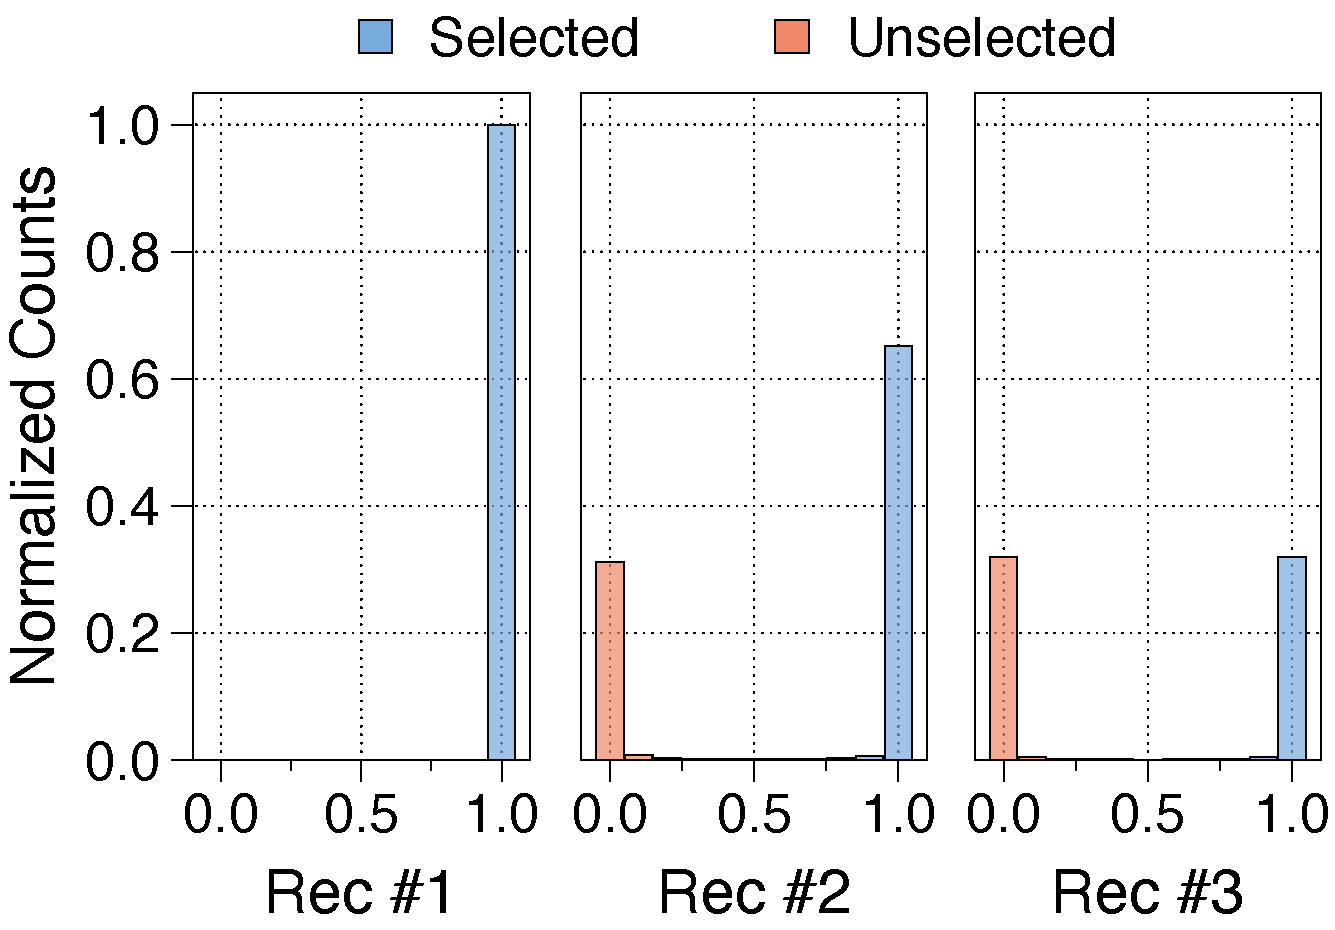
\includegraphics[width=\textwidth]{figs/weight_values/aux_loss_expert_app.pdf}
        \subcaption{Expert-choice (Auxiliary loss)}
    \end{subfigure}
    \centering
    \hspace{25pt}
    \begin{subfigure}[t]{0.4\textwidth}
    \captionsetup{justification=centering}
        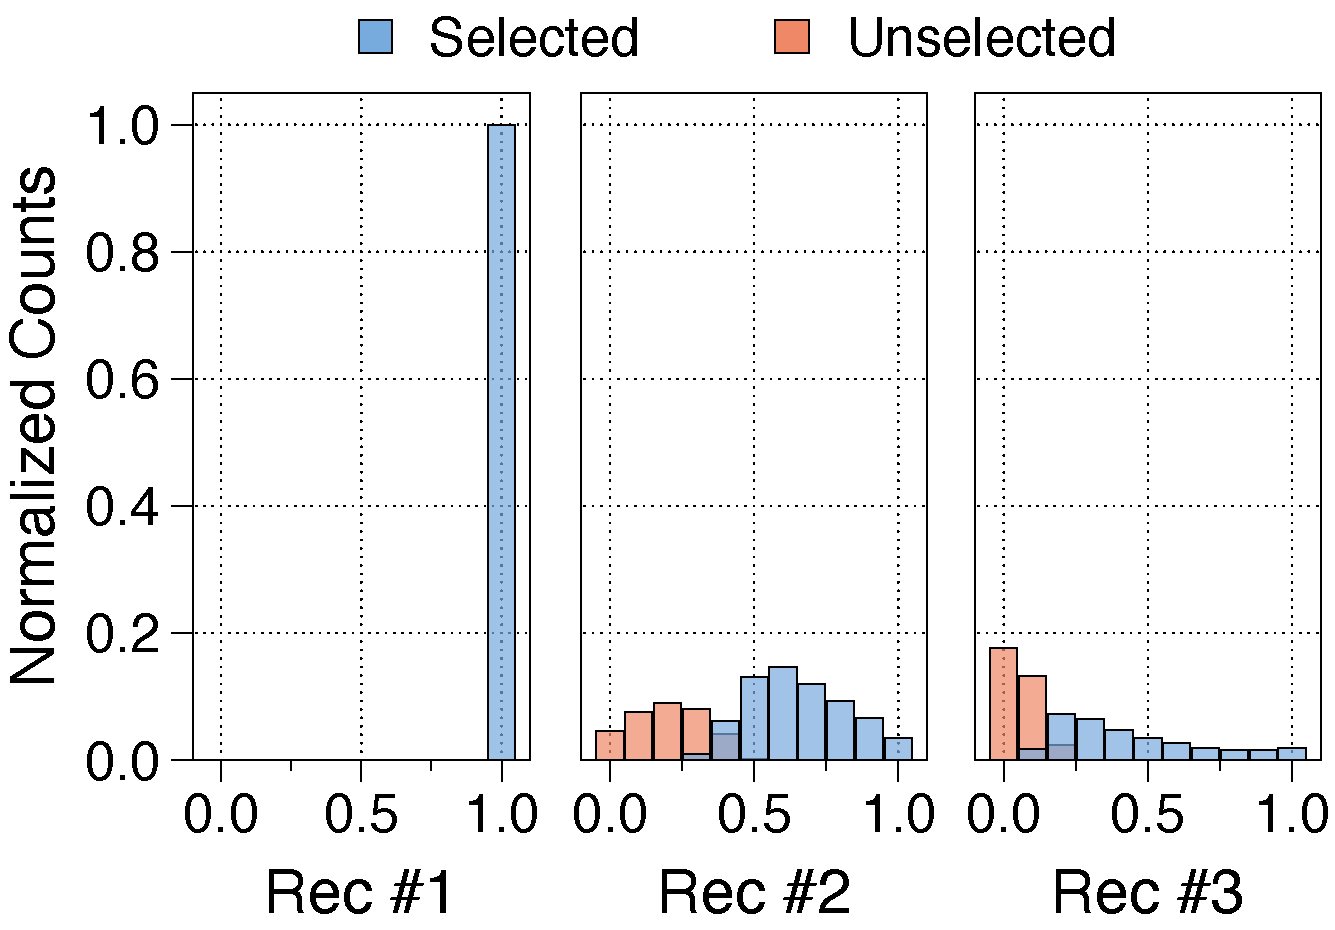
\includegraphics[width=\textwidth]{figs/weight_values/aux_router_expert_app.pdf}
        \subcaption{Expert-choice (Auxiliary router)}
    \end{subfigure}
    \centering
    \begin{subfigure}[t]{0.4\textwidth}
    \captionsetup{justification=centering}
        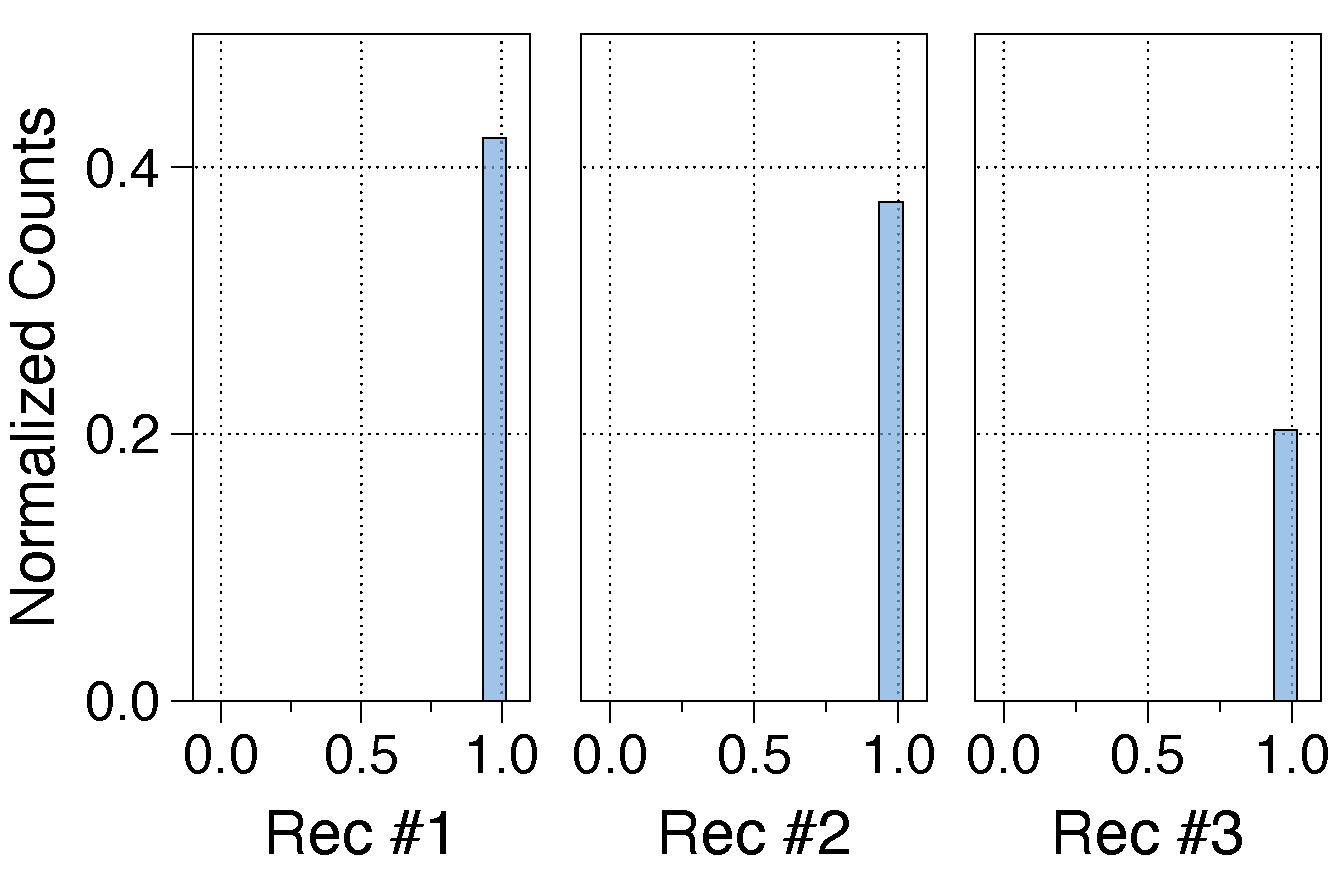
\includegraphics[width=\textwidth]{figs/weight_values/bal_loss_token_app.pdf}
        \subcaption{Token-choice (Balancing loss)}
    \end{subfigure}
    \centering
    \hspace{25pt}
    \begin{subfigure}[t]{0.4\textwidth}
    \captionsetup{justification=centering}
        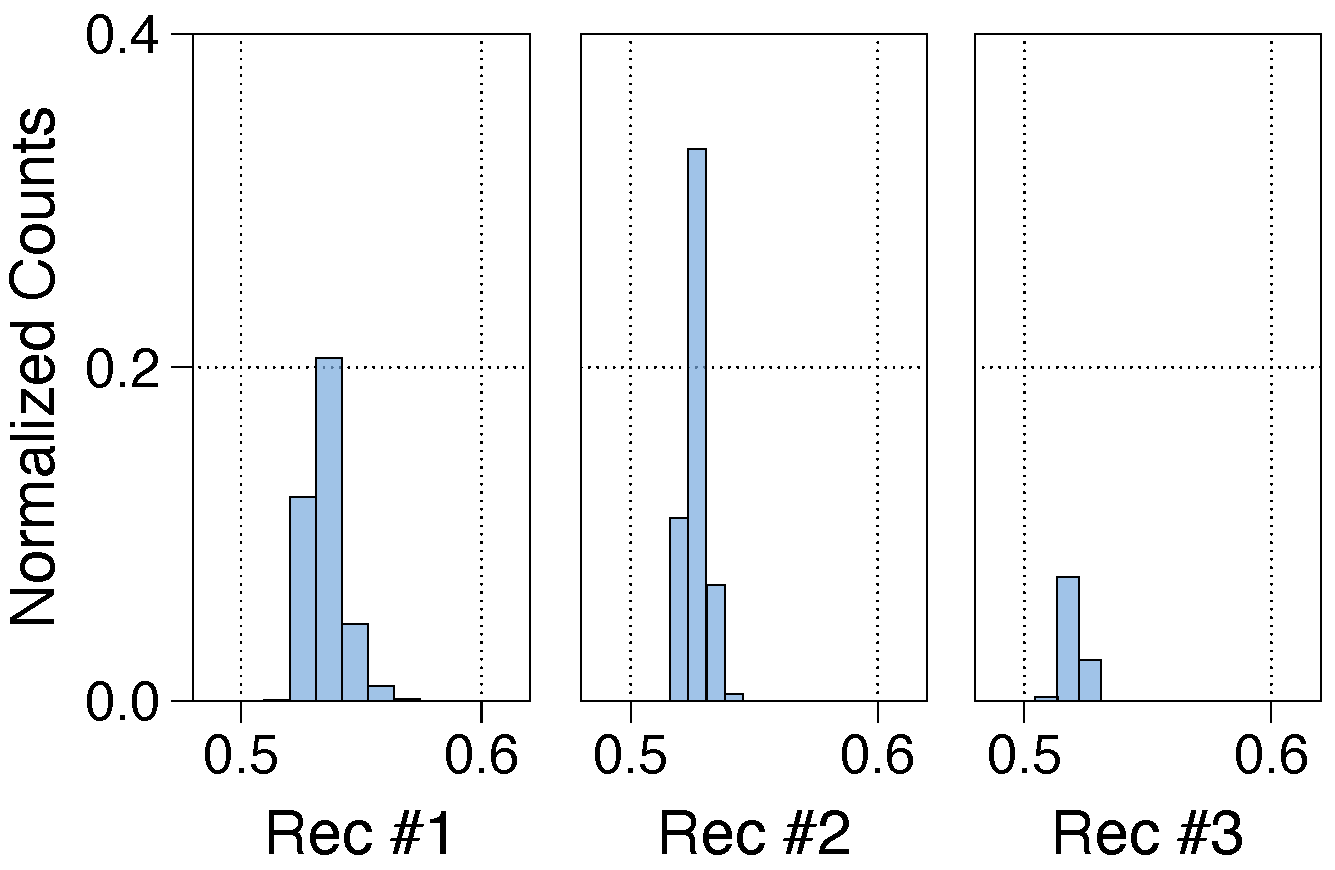
\includegraphics[width=\textwidth]{figs/weight_values/loss_free_token_app.pdf}
        \subcaption{Token-choice (Loss-free)}
    \end{subfigure}
    \caption{
    Distribution of router weights for selected and unselected tokens at each recursion step in expert-choice and token-choice MoR~($N_r$=3). All models use the recursion-wise KV caching strategy. The subplots show results for (a) expert-choice routing with auxiliary loss, (b) auxiliary router, (c) token-choice routing with balancing loss, and (d) loss-free algorithm. Each subplot uses the best hyperparameter settings identified in \autoref{tab:ablation_study_router}.
    }    
    \label{fig:weight_values_app}
\end{figure}




